
\begin{figure*}
\centering
\begin{tabular}{ccc}
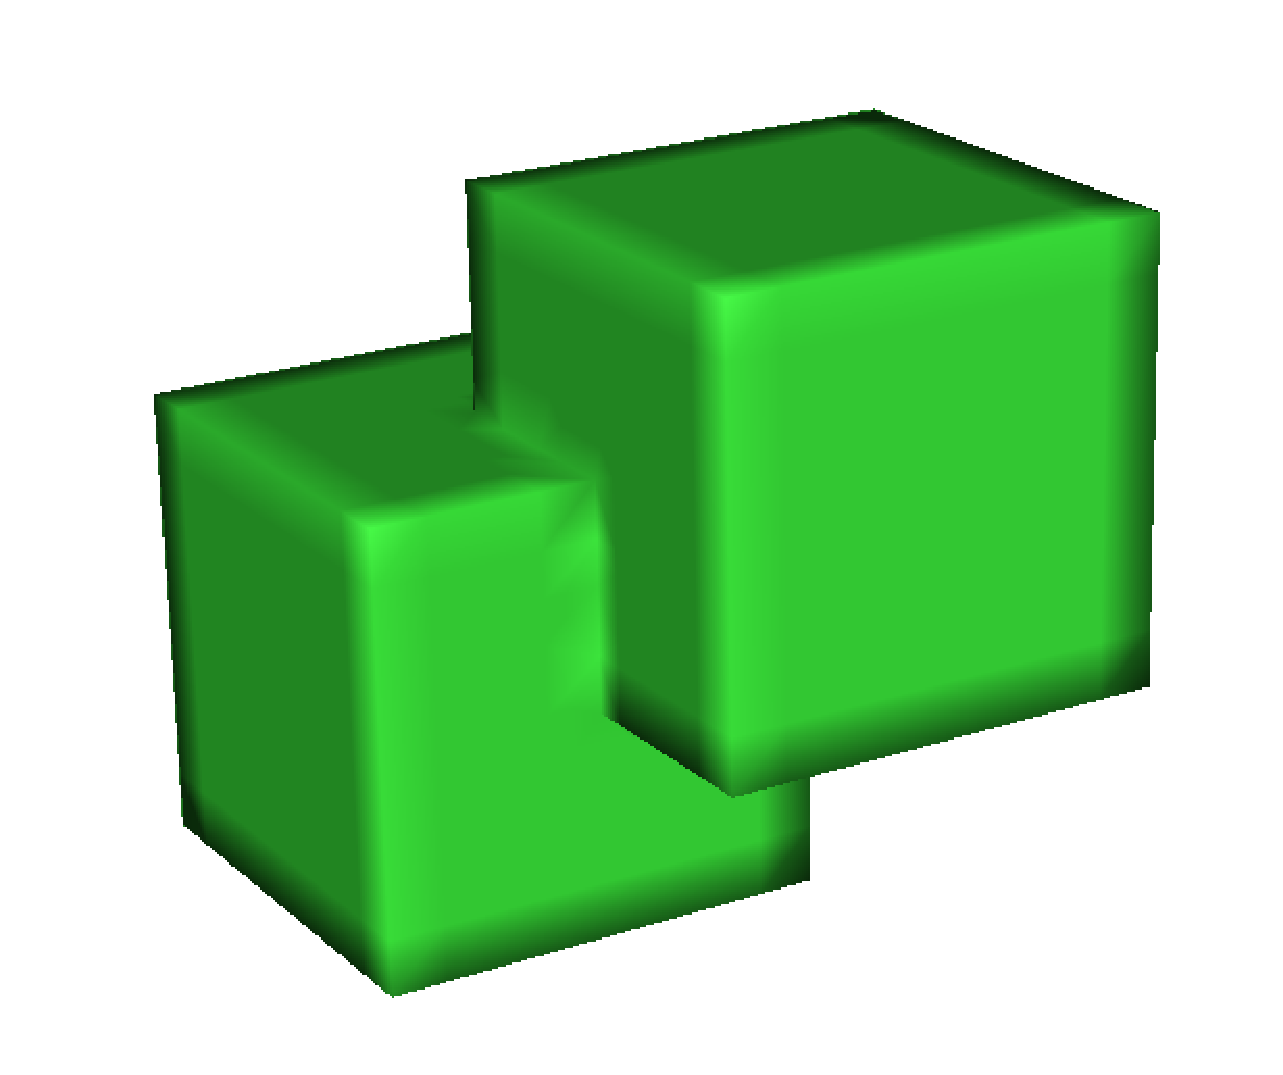
\includegraphics[width=1.5in]{images/twocubes.eps} \qquad &
\qquad
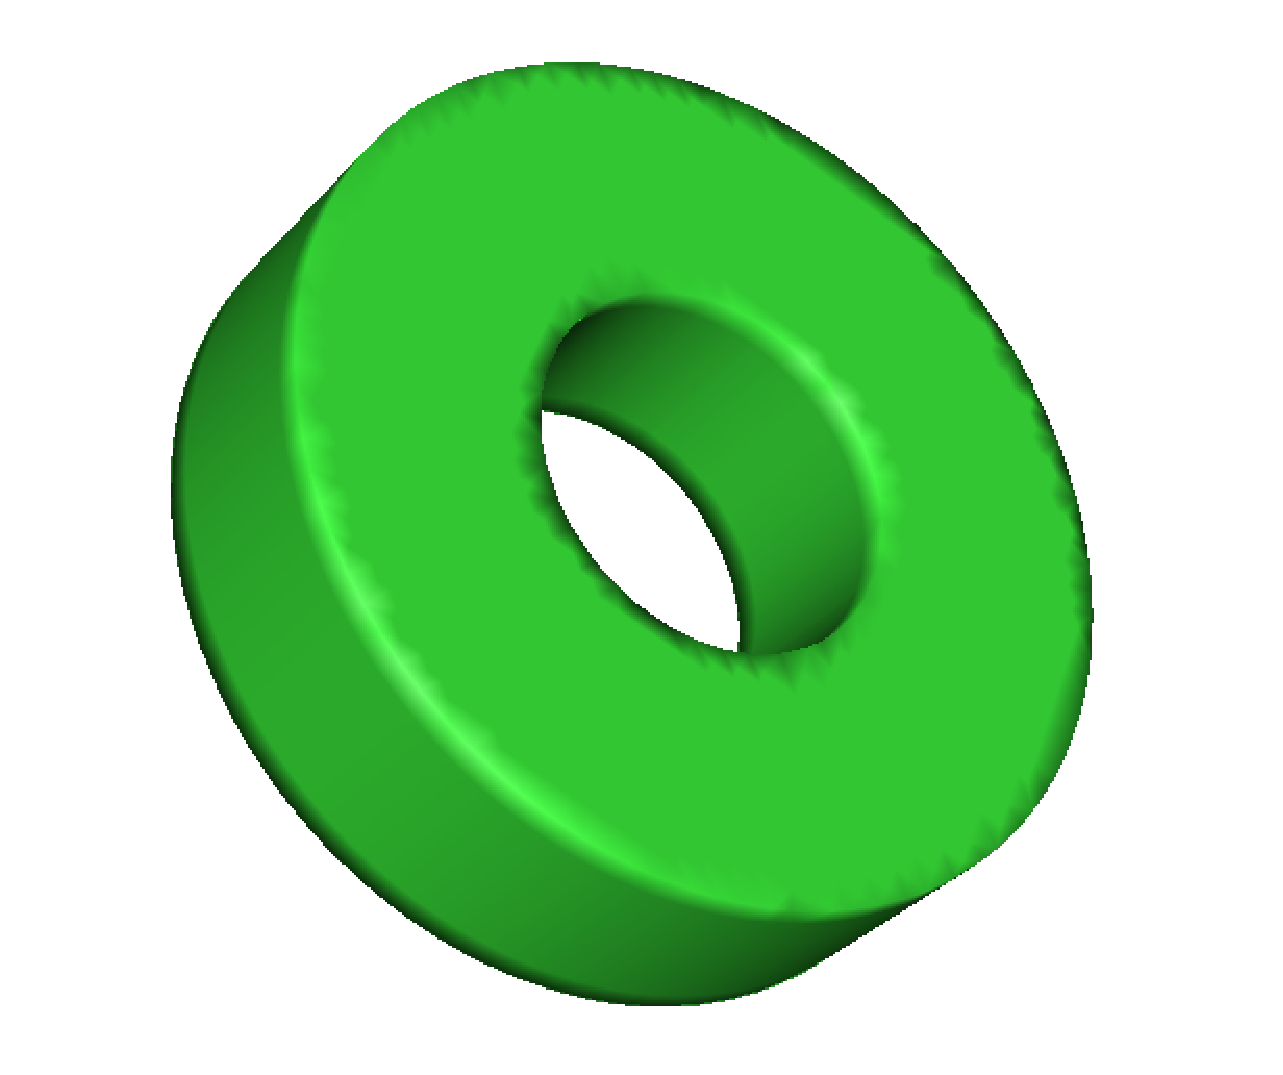
\includegraphics[width=1.5in]{images/annulus.eps}
\qquad &
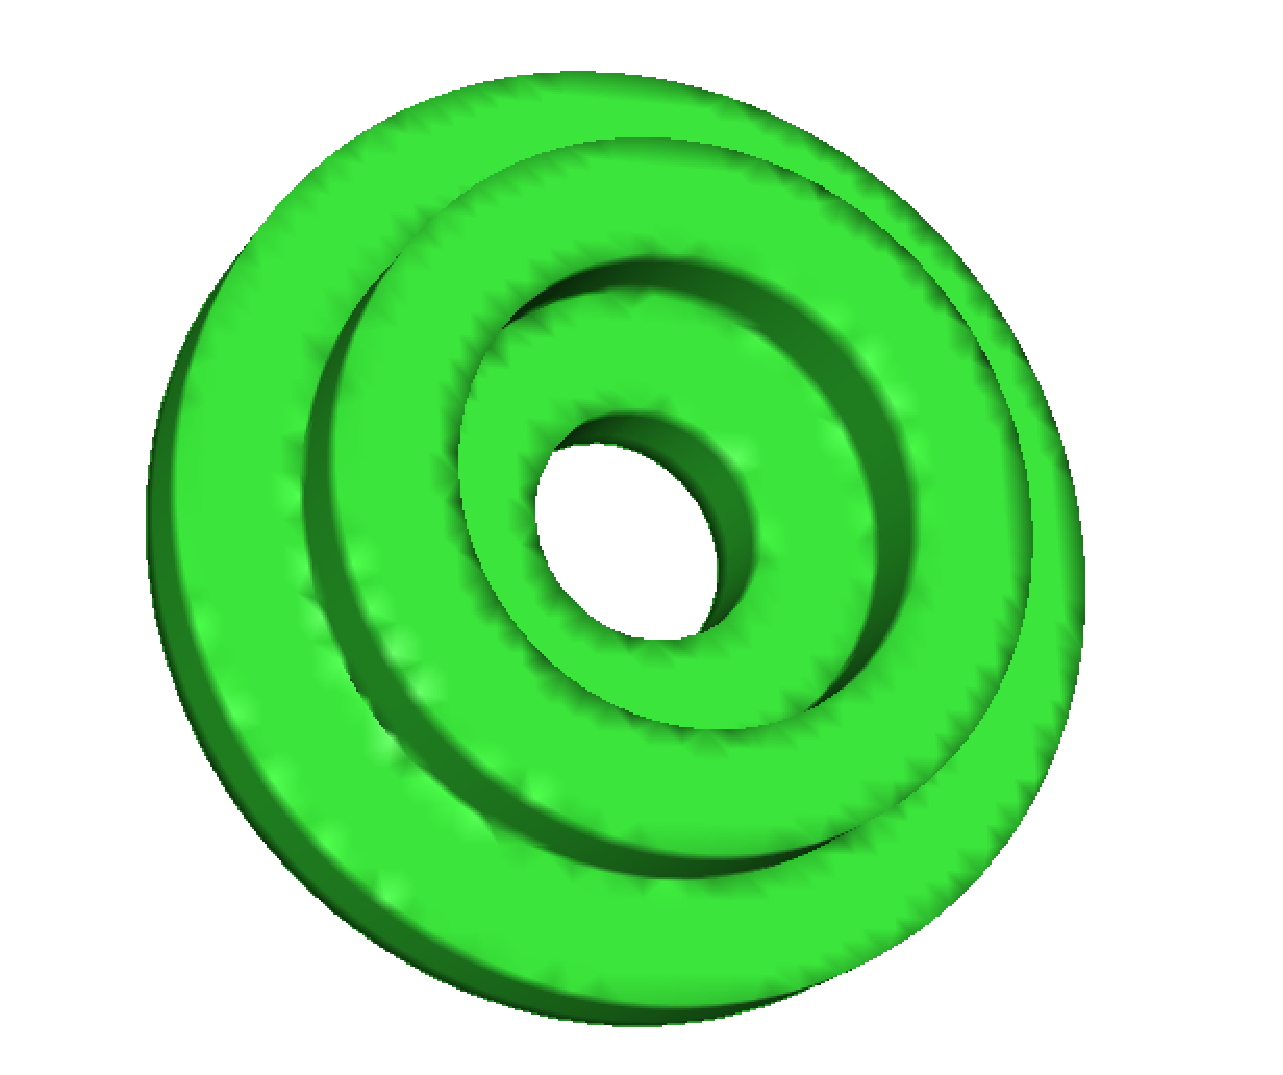
\includegraphics[width=1.5in]{images/flange.eps} \\

(a) Two cubes. & (b) Annulus. & (c) Flange. \\
\\
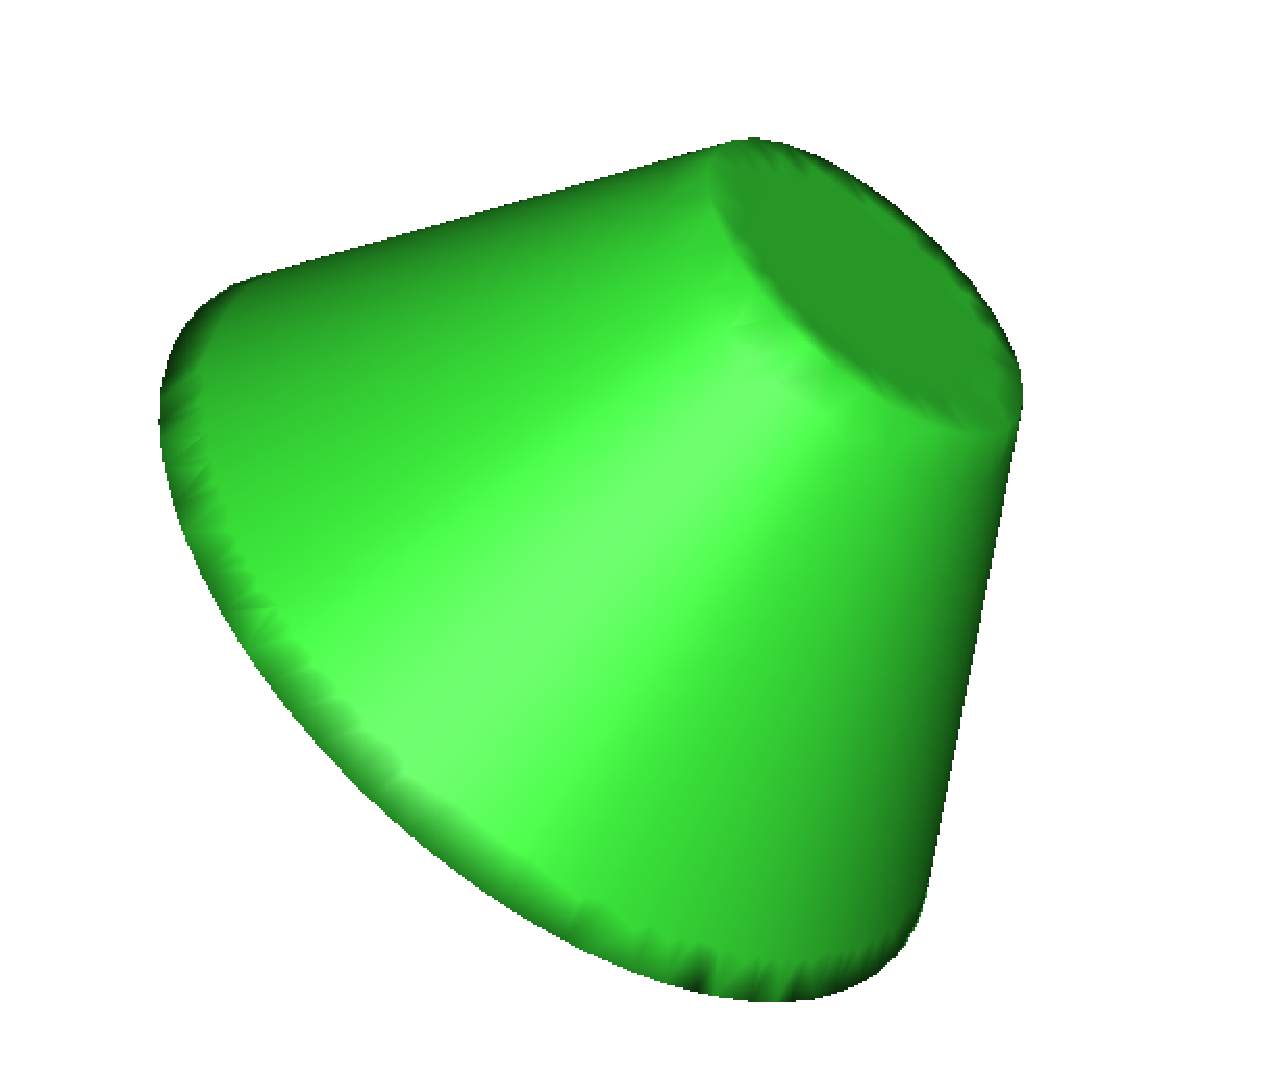
\includegraphics[width=1.2in]{images/frustrum.eps} \qquad &
\qquad
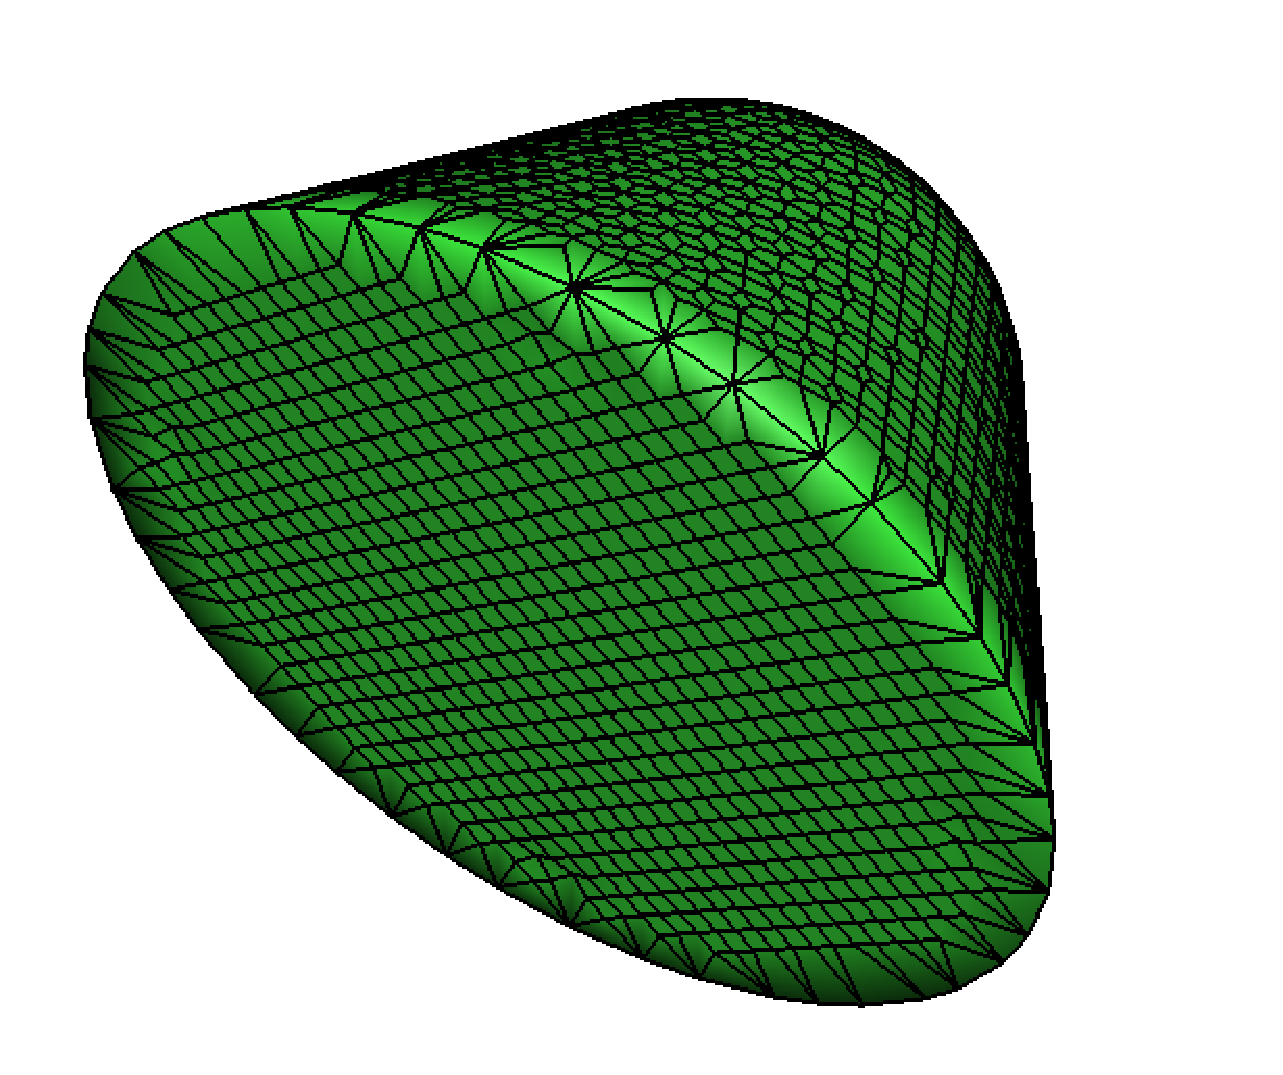
\includegraphics[width=1.2in]{images/smooth_tip_cone.eps} 
\qquad &
\qquad
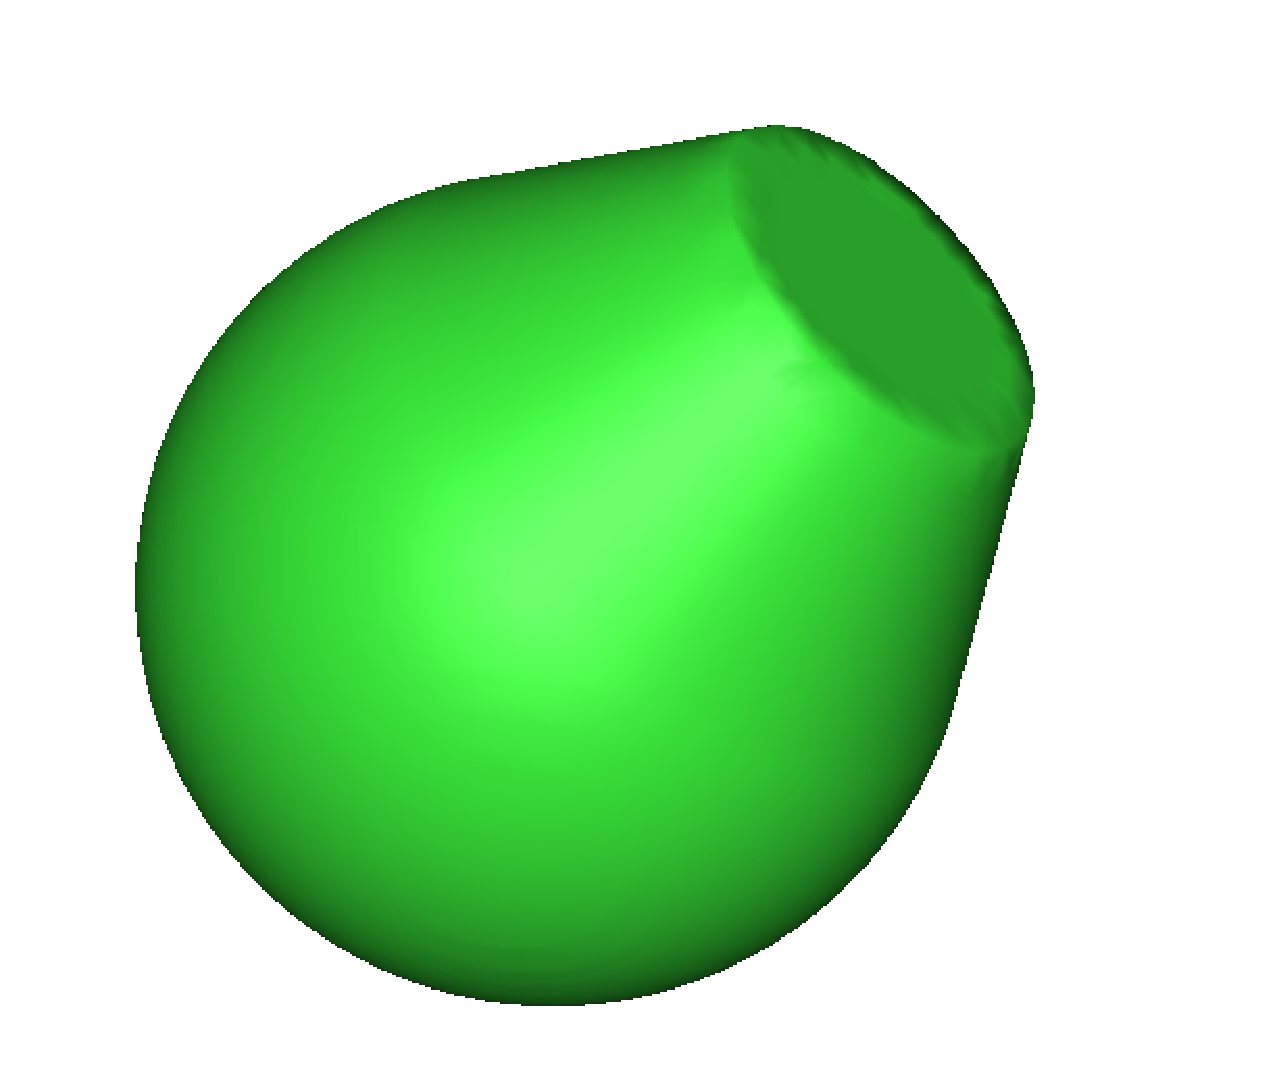
\includegraphics[width=1.2in]{images/cannon_iso.eps} \\
(d) Frustrum. & (e) Smooth tip cone. & (f) Cannon.
\end{tabular}
\caption{Isosurfaces constructed from synthetic test data sets.}
\label{fig:synthetic_data}
\end{figure*}

\newcommand{\fCYL}   {\emath{f^{Cyl}}}
\newcommand{\fCII}   {\emath{f^{Cyl \times 2}}}
\newcommand{\fPL}    {\emath{f^{Pl}}}
\newcommand{\fPLII}  {\emath{f^{Pl \times 2}}}
\newcommand{\fANN}   {\emath{f^{Ann}}}
\newcommand{\fCN}    {\emath{f^{Cone}}}
\newcommand{\fSCN}   {\emath{f^{SCone}}}
\newcommand{\fTCN}   {\emath{f^{TCone}}}
\newcommand{\fFR}    {\emath{f^{Fr}}}
\newcommand{\fX}     {\emath{f^{X}}}
\newcommand{\fCAN}   {\emath{f^{Can}}}
\newcommand{\NneqII} {\emath{N_{\neq 2}}}


\section{Experimental Results on Synthetic Data}\label{sec:synData}
\label{section:results}

\subsection{Synthetic Scalar and Gradient Data}
\label{section:synthetic}

To measure the quality of our reconstruction,
we used a number of synthetic scalar and gradient data sets.
(See Figure~\ref{fig:synthetic_data}.)
Given a point $p$,
let $f^{L_1}_{p}(q)$ be the $L_1$ distance from $p$ to $q$.
A {\em Cube} data set is generated by sampling $f^{L_1}_p$
and its gradients on vertices of the regular grid.

Level sets of $f^{L_1}_p$ are cubes whose edges are
parallel to the coordinate axes
and whose facets are orthogonal to those axes.
By rotating $f^{L_1}_p$ around $p$, 
we can generate a scalar field whose level sets are cubes
that are not axis-aligned.
By taking the minimum of two (rotated) scalar fields, 
$f^{L_1}_p$ and $f^{L_1}_{p'}$, 
centered around two different points, $p$ and $p$', respectively,
we get a scalar field whose level sets are the boundaries
of the unions of the two cubes.
(See Figure~\ref{fig:synthetic_data}(a).)
We call a regular grid sampling of such a scalar field
and its gradients a {\em TwoCubes} data set.
The isosurface of a TwoCubes data set has twenty 0-dimensional features,
fourteen of which are cube corners and six of which are ``saddle points''
where the two boundaries of two cubes meet.
We use the TwoCubes data sets with various rotations
as test sets for the reconstruction of 0-dimensional features.

Let $\ell$ be a line.
Let $\fCYL_{\ell}(q)$ be the Euclidean distance from point $q$ to $\ell$.
The level sets of $\fCYL_{\ell}(q)$ are infinite cylinders around $\ell$.
Let $\fCII_{\ell,r}(q)$ equal $|\fCYL_{\ell}(q) - r|$.
The level sets of $\fCII_{\ell,r}(q)$  are pairs of infinite cylinders
at equal distances from the cylinder of radius $r$ around $\ell$.
Let $\fPLII_{p,\ell}(q)$ be the (unsigned) distance from $q$ to the plane
that contains point $p$ and is orthogonal to line $\ell$.
Let $\fANN_{p,\ell,r}(q)$ be the maximum 
of $\fCII_{\ell,r}(q)$ and of $\fPLII_{p,\ell}(q)$.
The level sets are the boundaries of thickened annuli.
(See Figure~\ref{fig:synthetic_data}(b).)

The width of the thickened annuli defined by $\fANN_{p,\ell,r}$
equals their height.
We can adjust change the difference between the width and height
by adding constants to $\fCII_{\ell,r}$ or $\fPLII_{p,\ell}(q)$.
Let $\fANN_{p,\ell,r,c_1,c_2}(q)$ be the maximum 
of $\fCII_{\ell,r}(q)+c_1$ and of $\fPLII_{p,\ell}(q)+c_2$.
If $c_1$ is greater than $c_2$, 
then the height is $c_1-c_2$ units greater than the width.
If $c_2$ is greater than $c_1$, 
then the width is $c_2-c_1$ units greater than the height.

Define $\fFR_{p,\ell,r,c}(q)$ as the minimum
of $\fANN_{p,\ell,r,c,0}(q)$ and $\fANN_{p,\ell,r,0,c}(q)$.
The level sets of $\fFR_{p,\ell,r,c}(q)$ are the boundaries
of the unions of two thickened annuli.
(See Figure~\ref{fig:synthetic_data}(c).)
One annuli has height $c$ units greater than its width
while the other has width $c$ units greater than its height.
A {\em Flange} data set is a regular grid sampling of $\fFR_{p,\ell,r,c}(q)$
and its gradients.
The Flange data set has no 0-dimensional features.
We use the Flange data sets as test sets
for the reconstruction of 1-dimensional features.

We use two other types of data sets to test our algorithm on dihedral
angles other than $90^\circ$.
A cone is defined by an apex $p$, an axis direction $\zeta$,
and an angle $\alpha < 90^\circ$.
The cone is the union of all the rays from $p$ forming angle $\alpha$
with $\zeta$.
Let $\ell$ be the directed line through $p$ with direction $\zeta$,
i.e. the cone axis.
Let $\pi_{\ell}(q)$ be the projection of point $q$ on $\ell$.
Let $D_1(q)$ be the distance from $p$ to $\pi_{\ell}(q)$
and let $D_2(q)$ be the signed distance from $\pi_{\ell}(q)$ to $p$.
(The distance is negative if $\pi_\ell(q)-p$ points in the opposite
direction from $\zeta$.)
Define $\fCN_{p,\zeta,\alpha}(q)$ 
as $\cos(\alpha) D_1(q) - \sin(\alpha) D_2(q)$.
Function $\fCN_{p,\zeta,\alpha}(q)$ is the signed distance
from point $q$ to its orthogonal projection on the cone,
when that orthogonal projection exists.
The level sets of $\fCN_{p,\zeta,\alpha}(q)$ are cones
with axis $\ell$.

We truncate the cone by defining a plane orthogonal to $\ell$.
Let $p'$ be a point on ray $p+t\zeta$
where $\zeta$ is a unit vector.
Let $\fPL_{p',\zeta}(q)$ equal $(q-p') \cdot \zeta$,
the (unsigned) distance from $q$ 
to the plane containing $p'$ orthogonal to $\zeta$.
Define
\begin{equation*}
\fFR_{p,\zeta,\alpha,p'}(q) = 
\max \left ( \fCN_{p,\zeta,\alpha}(q), \fPL_{p',\zeta}(q), \fPL_{p',-\zeta}(q)
\right ) .
\end{equation*}
The level sets of $\fFR_{p,\zeta,\alpha,p'}(q)$ are frustra.
(See Figure~\ref{fig:synthetic_data}(d).)

The level sets of $\fFR_{p,\zeta,\alpha,p'}(q)$
have two closed curves forming 1-dimensional features.
The dihedral angle on one of these curves is $90^\circ + \alpha$
while the dihedral angle on the other is $90^\circ - \alpha$.
To generate a field with dihedral angles of $90^\circ + \alpha$
or $90^\circ - \alpha$, but not both,
we modify $\fFR_{p,\zeta,\alpha,p'}(q)$ so that the level sets
are capped by spheres at one end.

Define
\begin{align*}
\fSCN_{p,\zeta,\alpha,p'}(q) & =
\left \{
\begin{array}{ll}
|q-p'| & \mbox{ if } \angle(q,p',p) \le 90^\circ - \alpha,\\
\fCN_{p,\zeta,\alpha}(q) & \mbox{ if } 
  \angle(q,p',p) > 90^\circ - \alpha,
\end{array}
\right .
\\
\fTCN_{p,\zeta,\alpha}(q) & = 
\max \left ( \fSCN_{p,\zeta,\alpha,p'}(q), \fPL_{p',\zeta} \right ).
\end{align*}

A level set of $\fSCN_{p,\zeta,\alpha,p'}(q)$ is a cone
with its tip smoothed.
A level set of $\fSCN_{p,\zeta,\alpha,p'}(q)$ is a truncated cone
with its tip smoothed.
The level set has a single closed curve forming a 1-dimensional feature
with dihedral angle $90^\circ - \alpha$.
The {\em Smooth Tip Cone} data set is a regular sampling
of $\fTCN_{p,\zeta,\alpha,p'}(q)$ and its gradients.
We use Smooth Tip Cone data sets to evaluate reconstruction
of dihedral angles less than $90^\circ$.

Let $p'$ and $p''$ be points on the ray $p + t \zeta$ where
$|p-p'|$ is less than $(1-\sin(\alpha)) |p-p''|$.
Define
\begin{align*}
\fX_{p,\zeta,\alpha,p''}(q) & =
\left \{
\begin{array}{ll}
|q-p''| & \mbox{ if } \angle(q,p',p) > 90^\circ - \alpha,\\
\fCN_{p,\zeta,\alpha}(q) & \mbox{ if } \angle(q,p',p) \le 90^\circ - \alpha.
\end{array}
\right .
\\
\fCAN_{p,\zeta,\alpha,p',p''}(q) & =
\max \left ( \fX_{p,\zeta,\alpha,p''}(q), \fPL_{p',-\zeta} \right ) .
\end{align*}

A level set of $\fCAN_{p,\zeta,\alpha,p'}(q)$ has the shape of a cannon.
The level set has a single closed curve forming a 1-dimensional feature
with dihedral angle $90^\circ + \alpha$.
The {\em Cannon} data set is a regular sampling
of $\fCAN_{p,\zeta,\alpha,p'}(q)$ and its gradients.
We use Cannon data sets to evaluate reconstruction
of dihedral angles greater than $90^\circ$.



\begin{figure*}
\centering
\begin{tabular}{cccc}
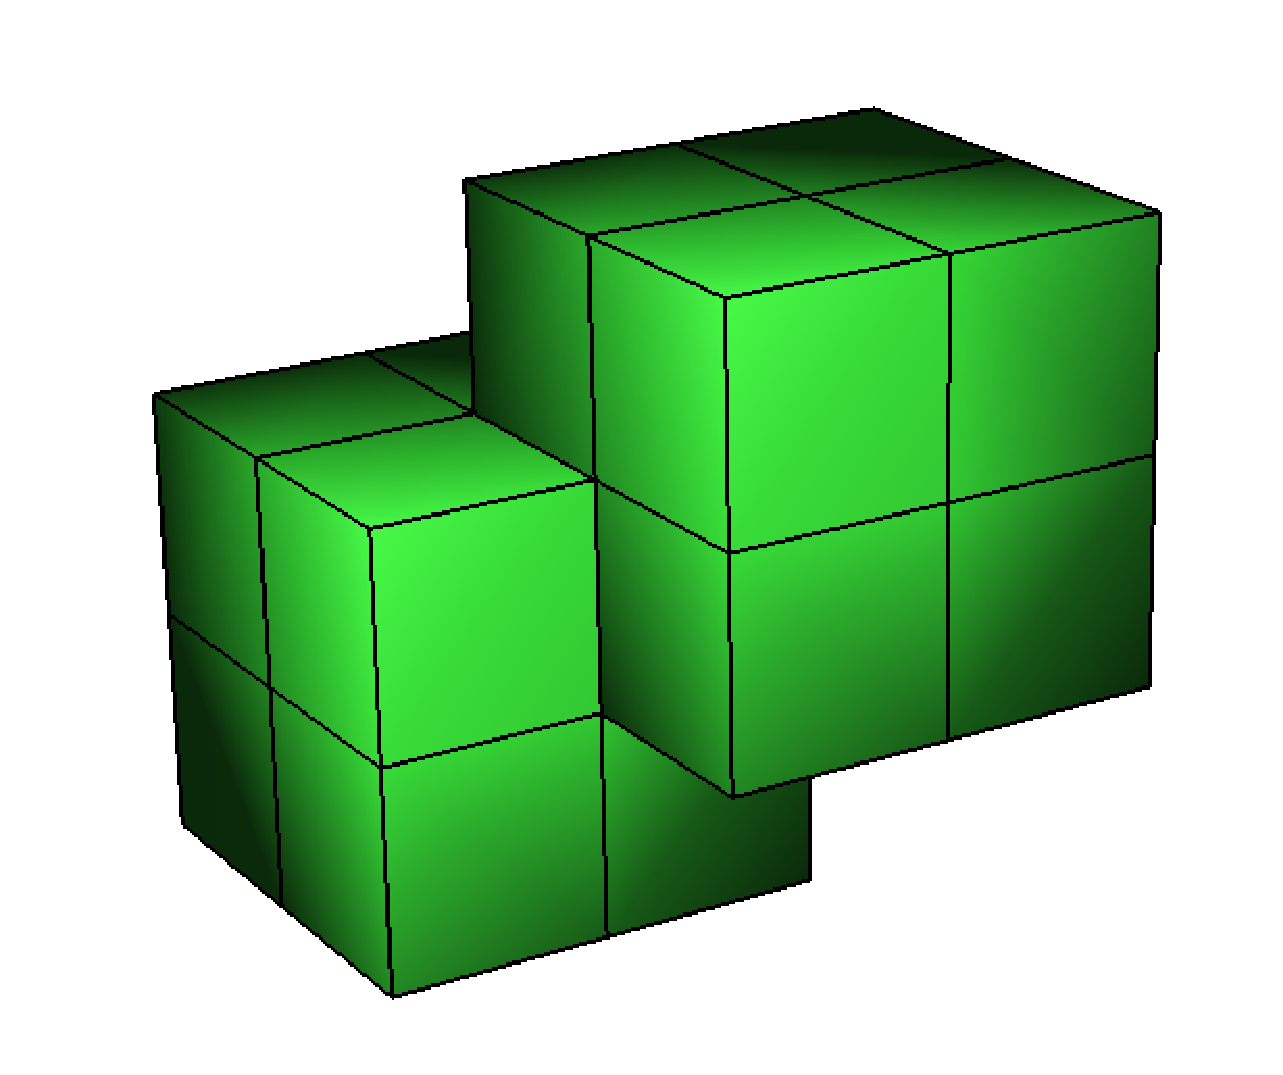
\includegraphics[width=1.6in]{images/twocubes_mesh.eps} &
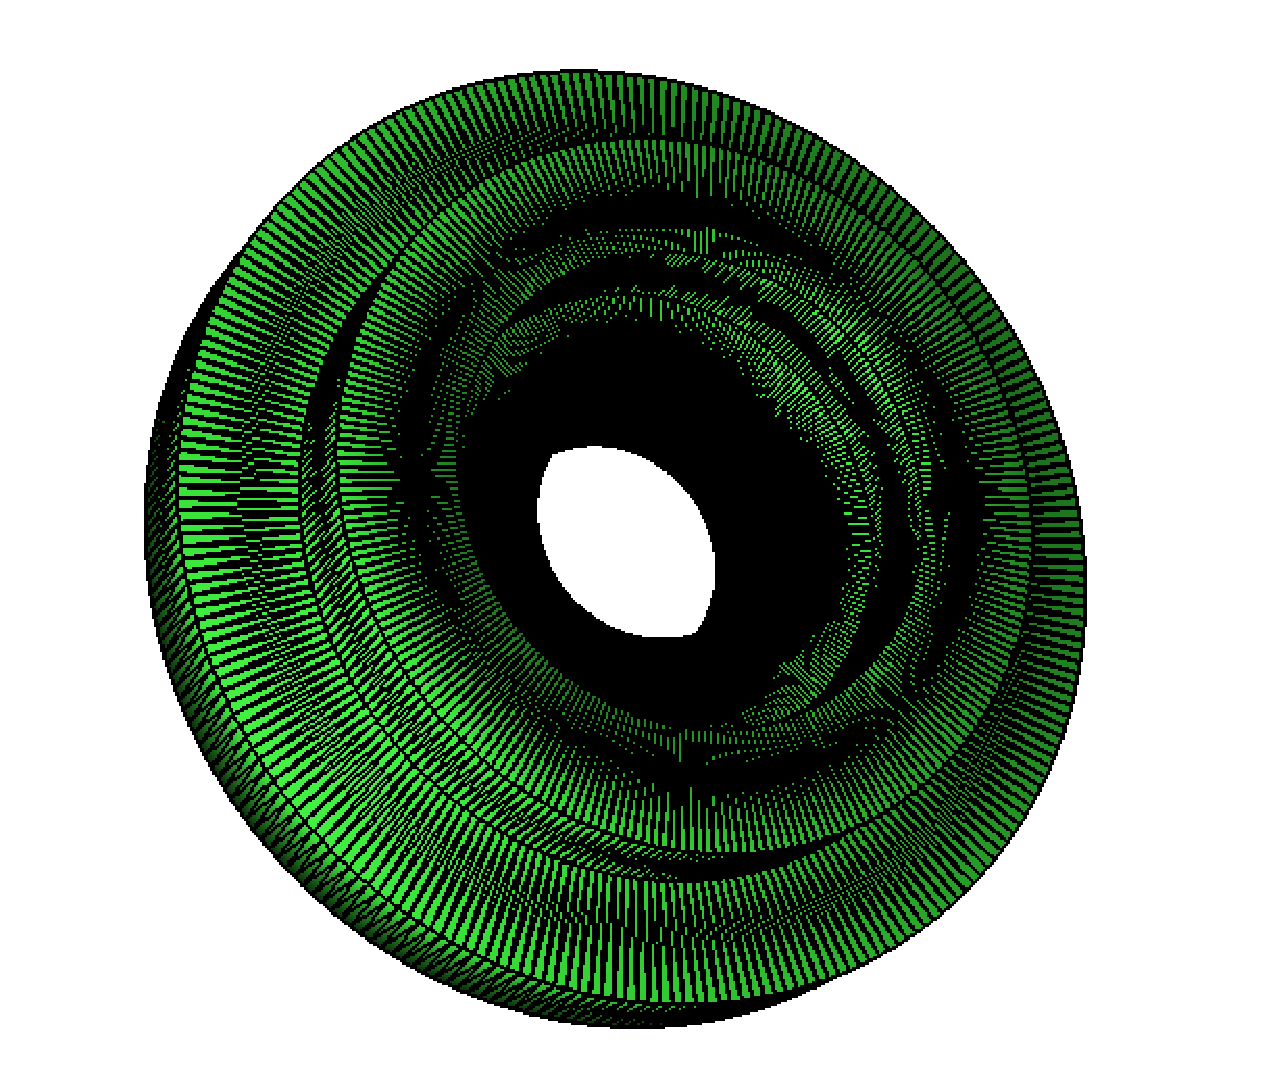
\includegraphics[width=1.6in]{images/flange_mesh.eps} &
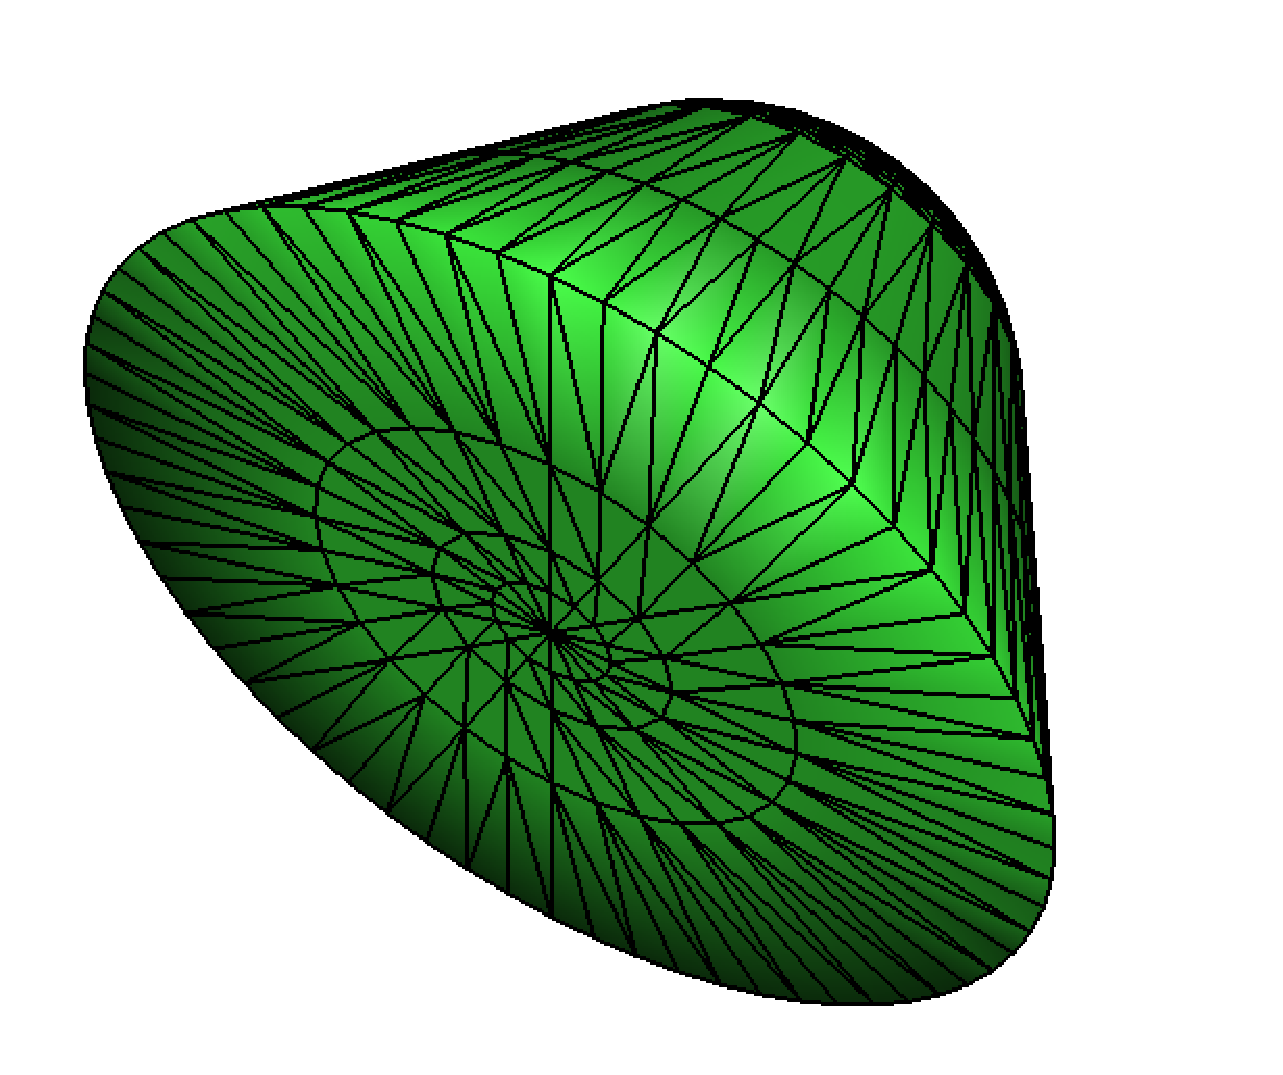
\includegraphics[width=1.6in]{images/smooth_tip_cone_mesh.eps} &
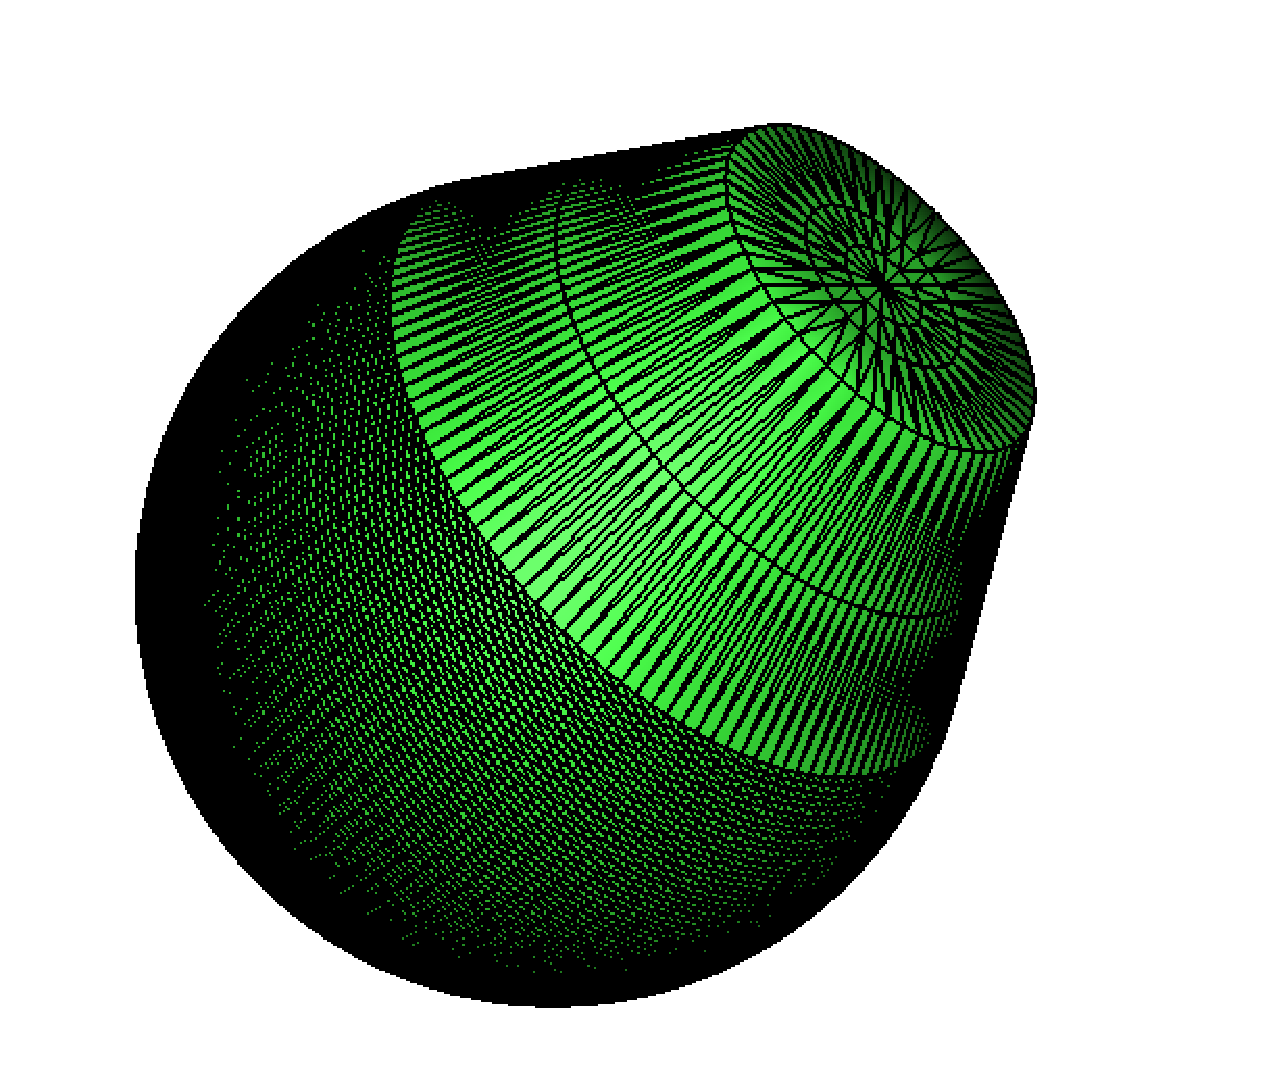
\includegraphics[width=1.6in]{images/cannon_mesh.eps}
\\
(a) Two cubes. & (b) Flange. & (c) Smooth tip cone. & (d) Cannon. \\
\end{tabular}
\caption{Polyhedral meshes representing level sets.}
\label{fig:mesh}
\end{figure*}


\begin{table*}[t]
\centering
\begin{tabular}{|l||r|c|c|r|r|r|r|}
\hline
              & \centercol{Num} & & & \centercol{Avg Num} 
                                     & \centercol{Avg Num} 
                                         & \centercol{Avg Num} & \\
Data Set Type & Data Sets & Grid Size & Isovalue 
                                 & \centercol{Active Cubes} 
                                    & \centercol{Iso Vert} 
                                        & \centercol{Iso Tri} 
                                             & \centercol{Avg Time} \\
\hline
\hline
TwoCubes & 34 & \gDim{150} & 20.1 & 25K & 22K & 45K & 0.8 sec \\
\hline
Flange & 40 & \gDim{200} & 10.1 & 90K & 75K & 150K & 1.8 sec \\
\hline
Smooth Tip Cone & 15 & \gDim{100} & 10.2 & 4K & 3.5K & 7K & 0.2 sec \\
\hline
Cannon & 15 & \gDim{100} & 0.0 & 7K & 7K & 14K & 0.2 sec \\
\hline
%setA.nhdr
%1599600 grid cubes.
%Isovalue 22000.  26049 isosurface vertices.  51170 isosurface simplices.
%25584 (1%) non-empty cubes.
%Wrote output to file: setA.isov=22000.off
Motorcyle Engine & 1 & $200 \times 129 \times 62$ 
   & 22000 & 25k& 26k& 51k& 1.9\\
\hline
%160uCT.crop1
%10578000 grid cubes.
%Isovalue 4000.  527574 isosurface vertices.  1039534 isosurface simplices.
%519308 (4%) non-empty cubes.
%Wrote output to file: 160uCT.crop1.aniso.isov=4000.off
Volt & 1 & $411 \times 431 \times 61$ & 4000& 519k& 527k& 1039k& 39.01\\
\hline
%%% CMM.setA.nhdr in folder industrial CT
%48555195 grid cubes.
%Isovalue 20000.  863987 isosurface vertices.  1726046 isosurface simplices.
%861673 (1%) non-empty cubes.
CMM & 1 & $500 \times 500 \times 196$ & 20000& 861k& 863k& 1726k& 60.075\\
\hline
\end{tabular}

\caption{Test data set sizes, isovalues, and average statistics
on isosurfaces produced by SHREC.
Average number of active cubes, 
average number of isosurface vertices,
average number of isosurface triangles,
and average SHREC running time.
All isosurface quadrilaterals are triangulated
before counting the number of isosurface triangles.
Because SHREC merges isosurface vertices, the average number of isosurface
vertices is less than the average number of active cubes.
}

\label{table:datasets}

\end{table*}

\subsection{Gradients}

Algorithm SHREC requires gradients at the grid vertices.
Exact formulas can be given for gradients
for each of the scalar fields described in the previous section.
However, if scalar data is acquired from scanning devices such as CT scanners,
only scalar information is available.
In~\cite{bw-crgsd-15},
we describe an algorithm, Religrad, for constructing a set 
of reliable gradients from scalar data.
We evaluated SHREC both on gradients computed by exact formulas
and on the gradients produced by Religrad from the scalar data.

\subsection{Measurements}

For each test scalar field $f$ and test isovalue $\sigma$,
we constructed a polygonal mesh which represented the level set,
$f^{-1}(\sigma)$.
(See Figure~\ref{fig:mesh}.)
The polygonal mesh was designed specifically for each surface
to accurately represent the 0-dimensonal and 1-dimensional features
on the surface.

To compare isosurfaces constructed by different software on different scales,
we rescaled every isosurface and polygonal mesh to lie in the unit cube.
Our isosurfaces were computed from grids 
of $150 \times 150 \times 150$ or $200 \times 200 \times 200$
so this rescaled the cube size to about $0.005$ units.
We computed the angular distance in the extended neighborhood $\epsilon$
as defined in Section~\ref{section:angular_distance}
between each isosurface and the corresponding polygonal mesh.
We set $\epsilon$ equal to $0.01$ or about twice the cube size
for the extended neighborhood.

We also used the degree test as described in~\cite{bw-cisec-13}
to measure errors in reconstructing sharp features.
We extracted the 1-skeleton of isosurface edges with dihedral angle 
less than $140^\circ$ and counted the number of vertices in the 1-skeleton
with degree other than two.
For an isosurface $\Sigma$,
let $\NneqII(\Sigma)$ be the number of vertices in the 1-skeleton
with degree other than two.
Isosurfaces from the Flange, Smooth Tip Cone and Cannon data sets
should have had zero vertices with degrees other than two.
The number of degree errors for these isosurfaces is $\NneqII(\Sigma)$.
Isosurfaces from the TwoCubes data sets should have had exactly
twenty vertices with degrees other than two.
The number of degree errors for these isosurfaces is $|\NneqII(\Sigma)-20|$.

\begin{figure}[tb]
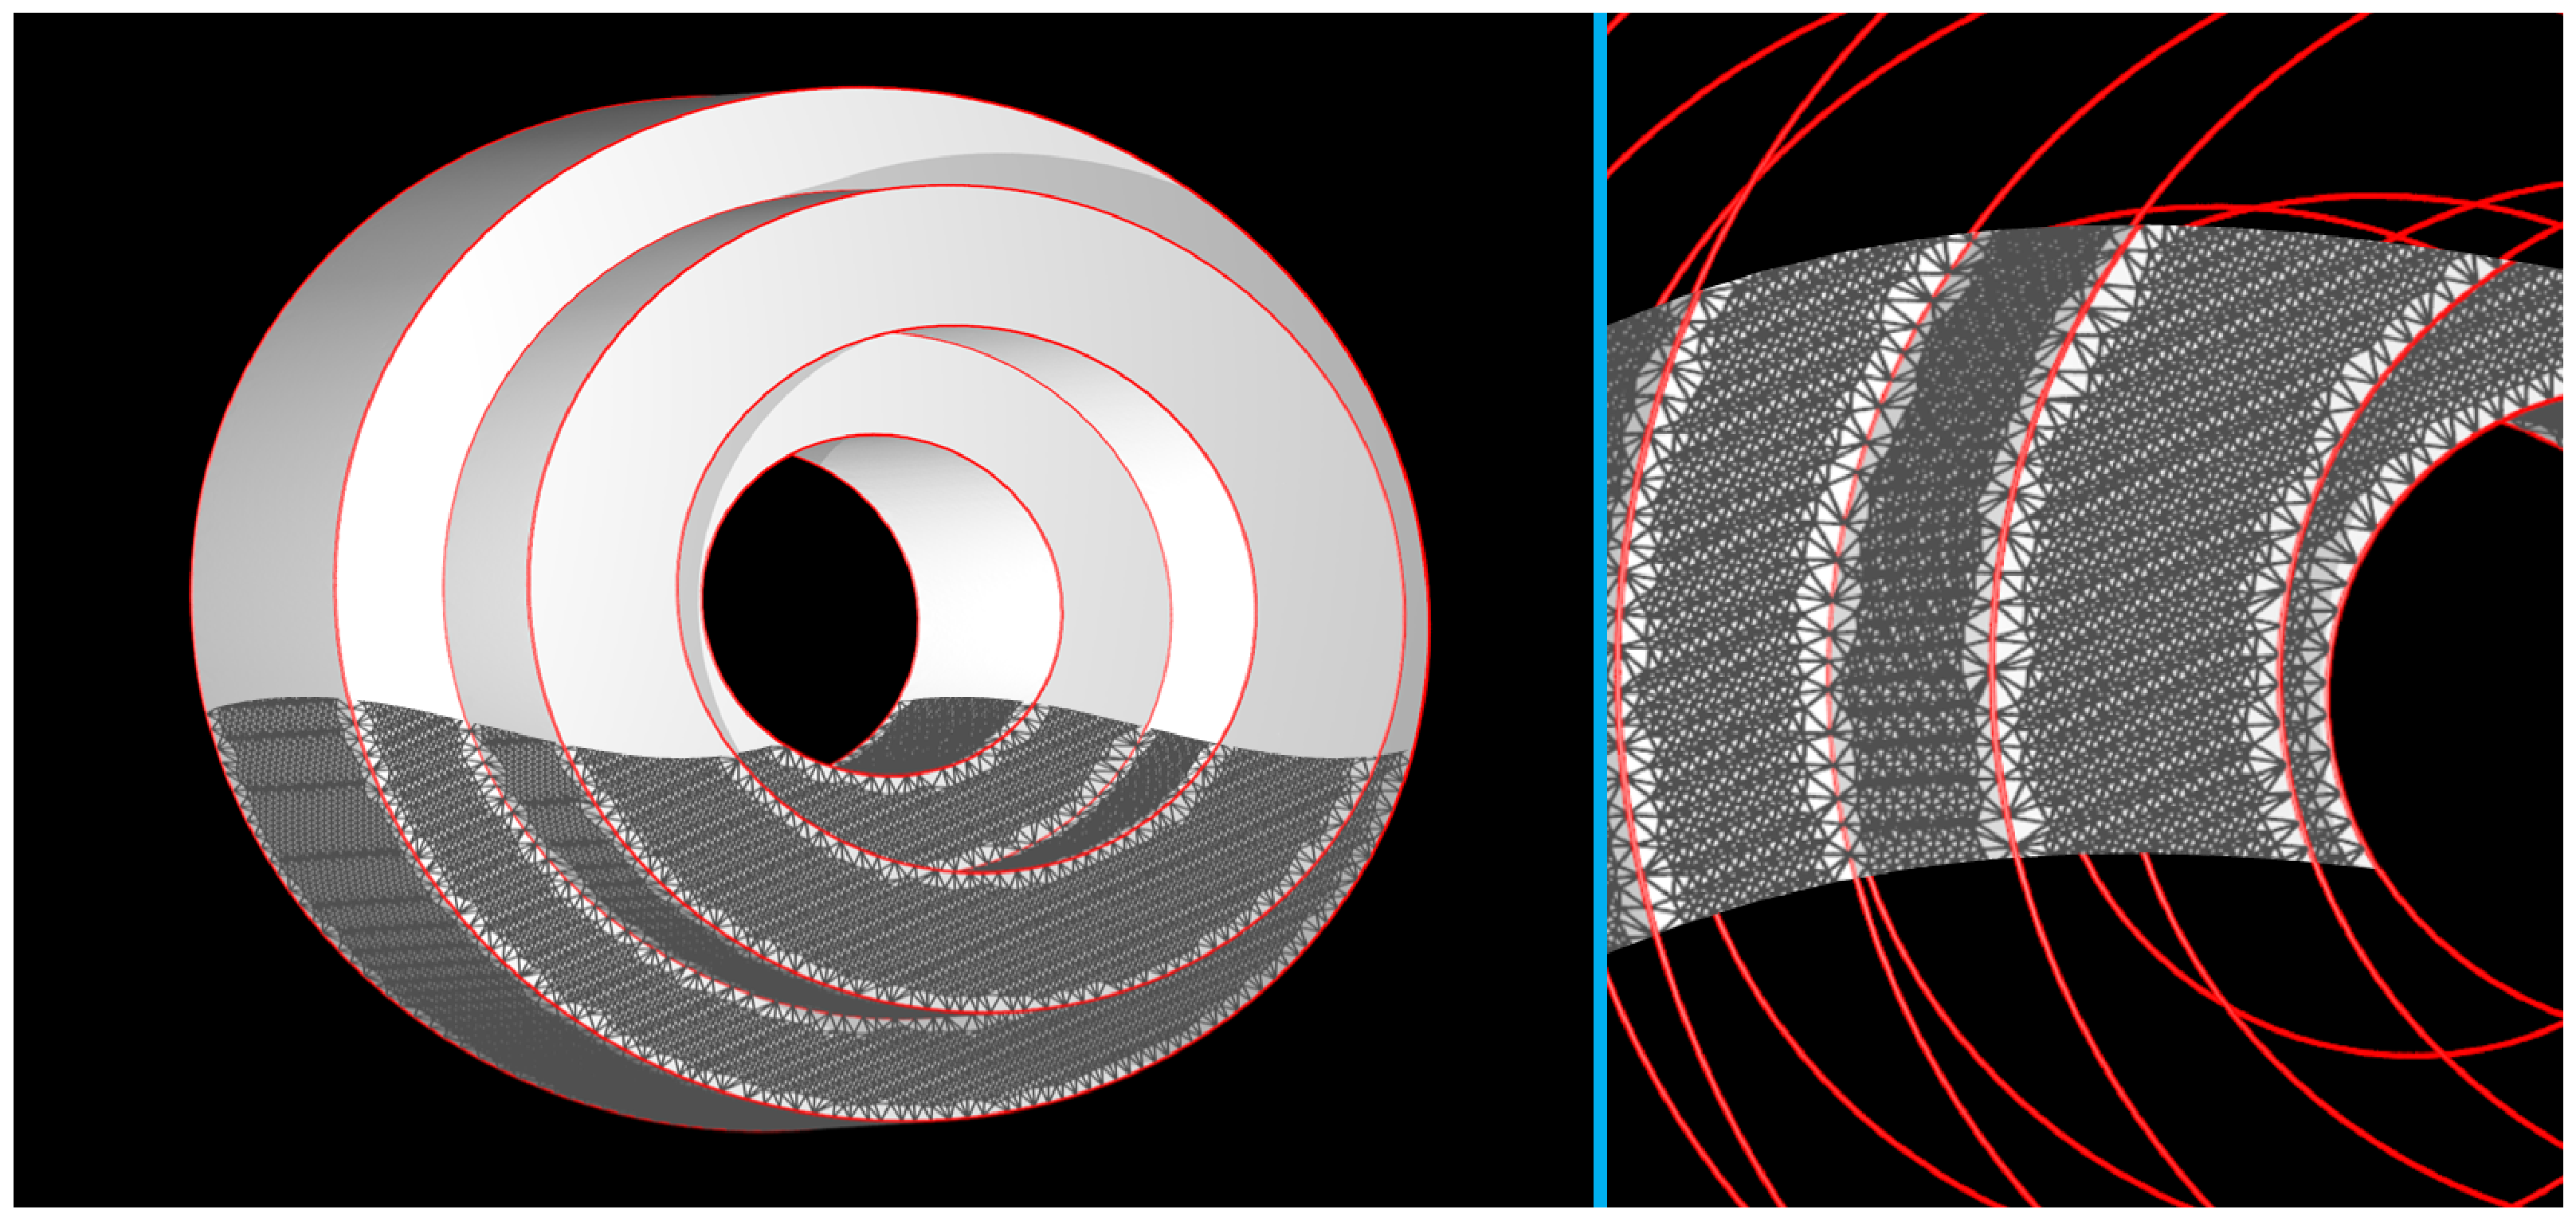
\includegraphics[width=\linewidth]{images/shrecFlangeCombine2.eps}
\caption{SHREC Flange isosurface. ``Sharp" edges (with dihedral angle less than $140^\circ$) are marked in red. 
``Smooth" edges are in dark grey. The magnified region shows a blend of the ``sharp" edges with a subset of the ``smooth" edges.}
\label{fig:flange1}
\end{figure}


\begin{figure*}[tp]
\centering	

	\subfloat[]{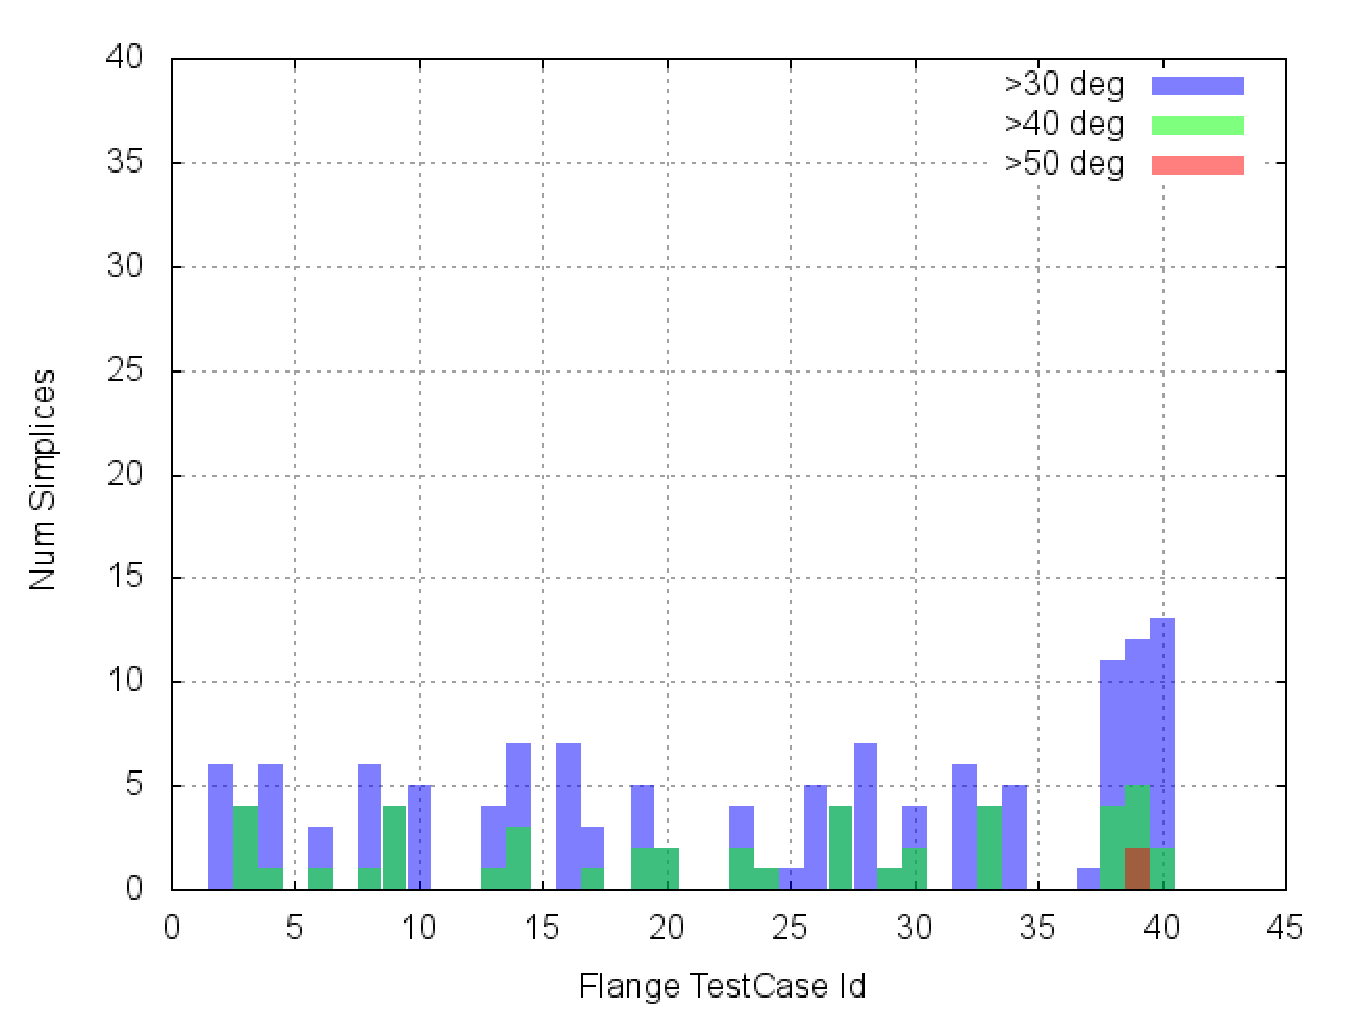
\includegraphics[width=0.33\linewidth]{images/flangeAngle1b.eps}\label{fig:flangeAngle1}}
	\subfloat[]{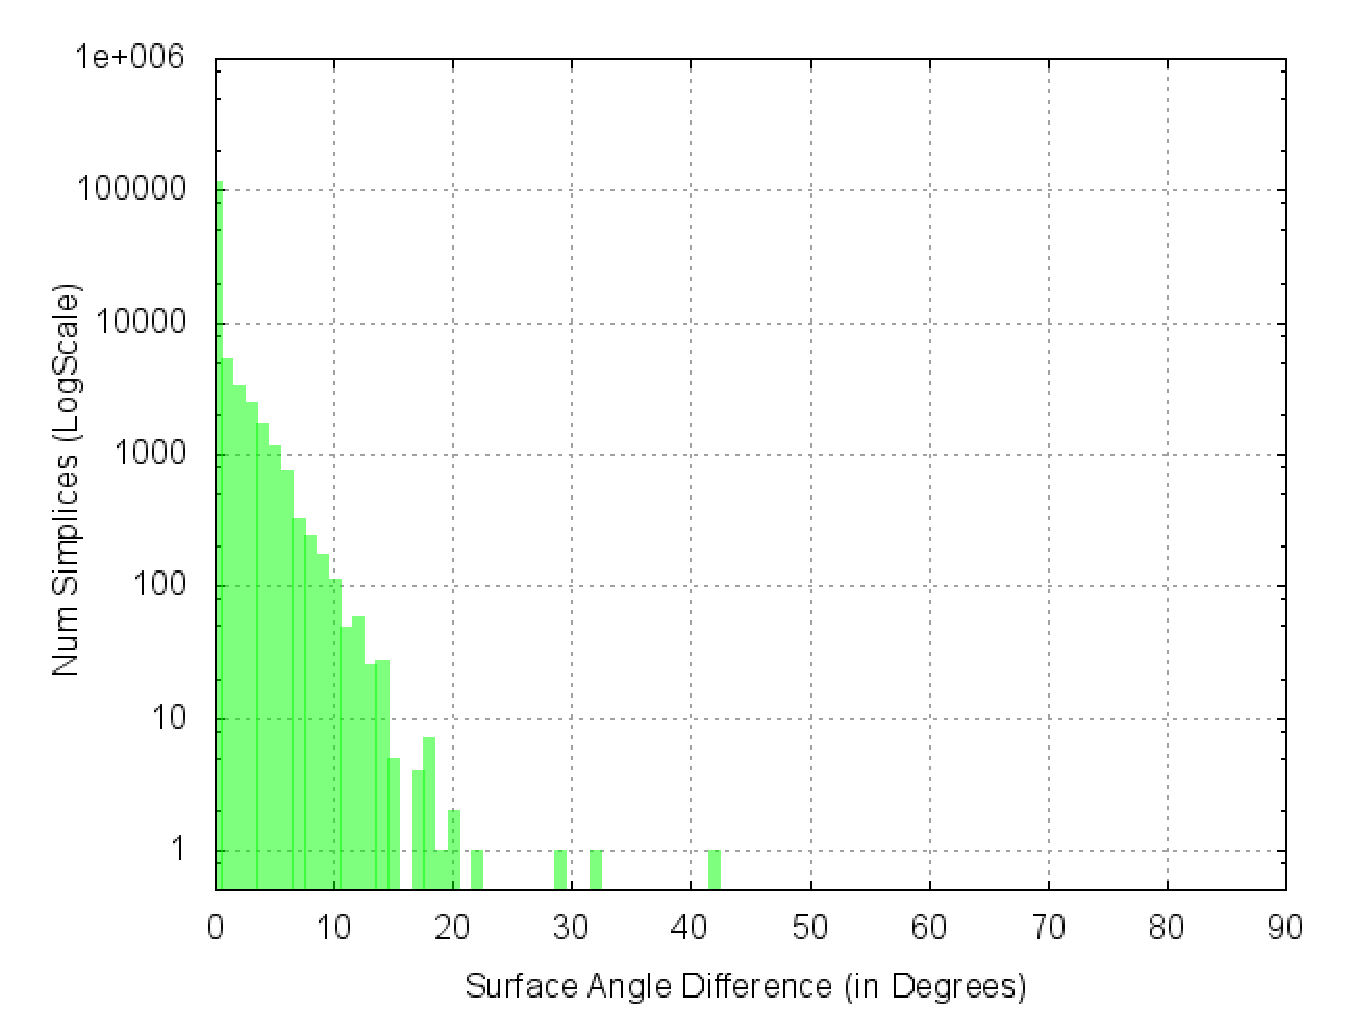
\includegraphics[width=0.33\linewidth]{images/flangeAngle2.eps}\label{fig:flangeAngle2}}
	\subfloat[]{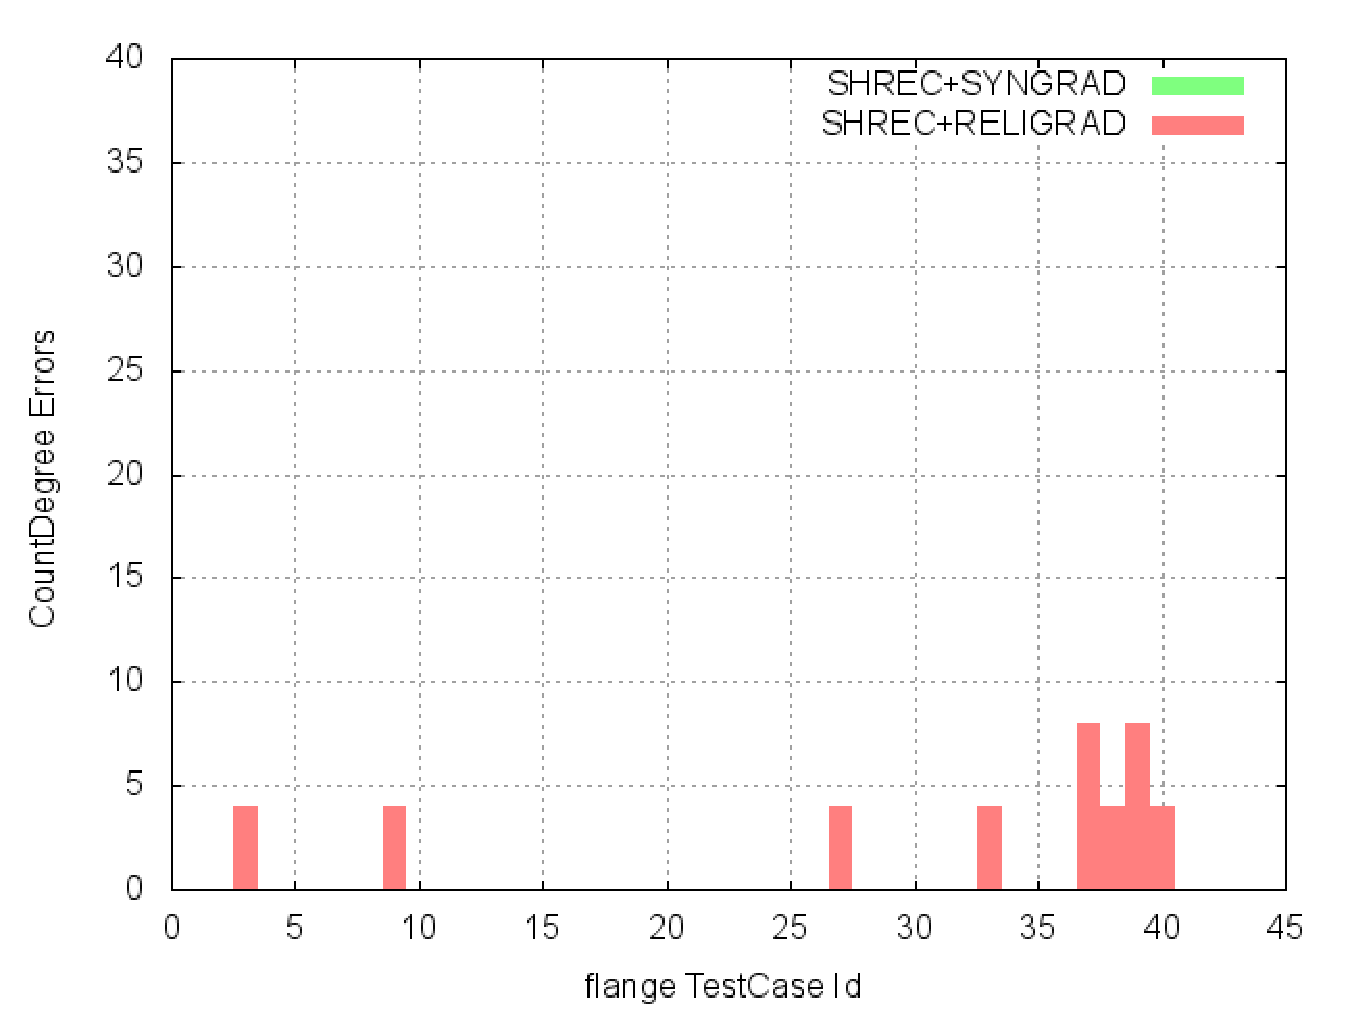
\includegraphics[width=0.33\linewidth]{images/flangeAngle3b.eps}\label{fig:flangeAngle3}}

\caption{Results of SHREC using Religrad gradients on 40 Flange datasets. 
(a) Number of triangles with angle difference 
to polygonal mesh above 30, 40 and 50 degrees. 
(b) Distribution of triangle normal differences for test case 16.
(Isosurface has approximately $133K$ triangles.)
(c) Number of degree errors in 1-skeleton of sharp edges.
}

\label{fig:flangeAngle}

\vspace{4em}

\begin{tabular}{cc}
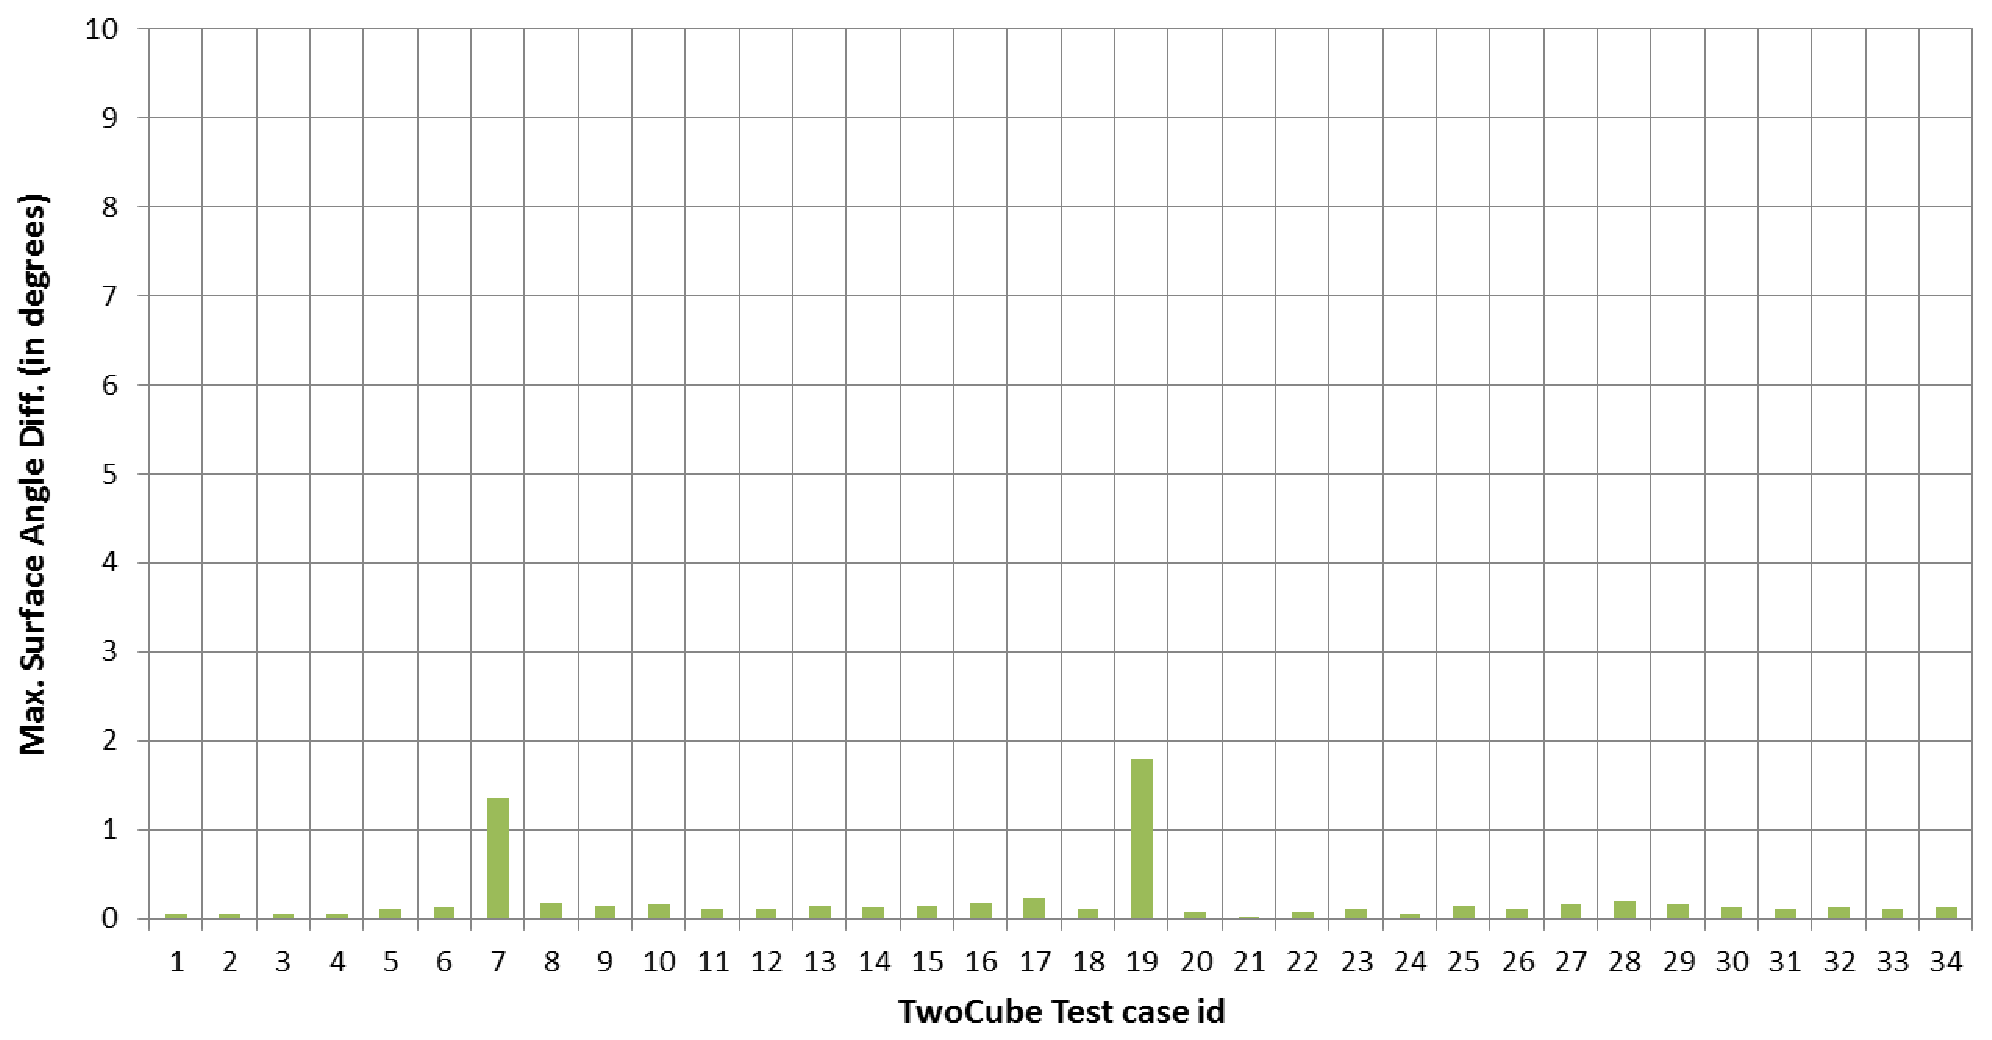
\includegraphics[width=0.45\linewidth]{images/tw1.eps} &
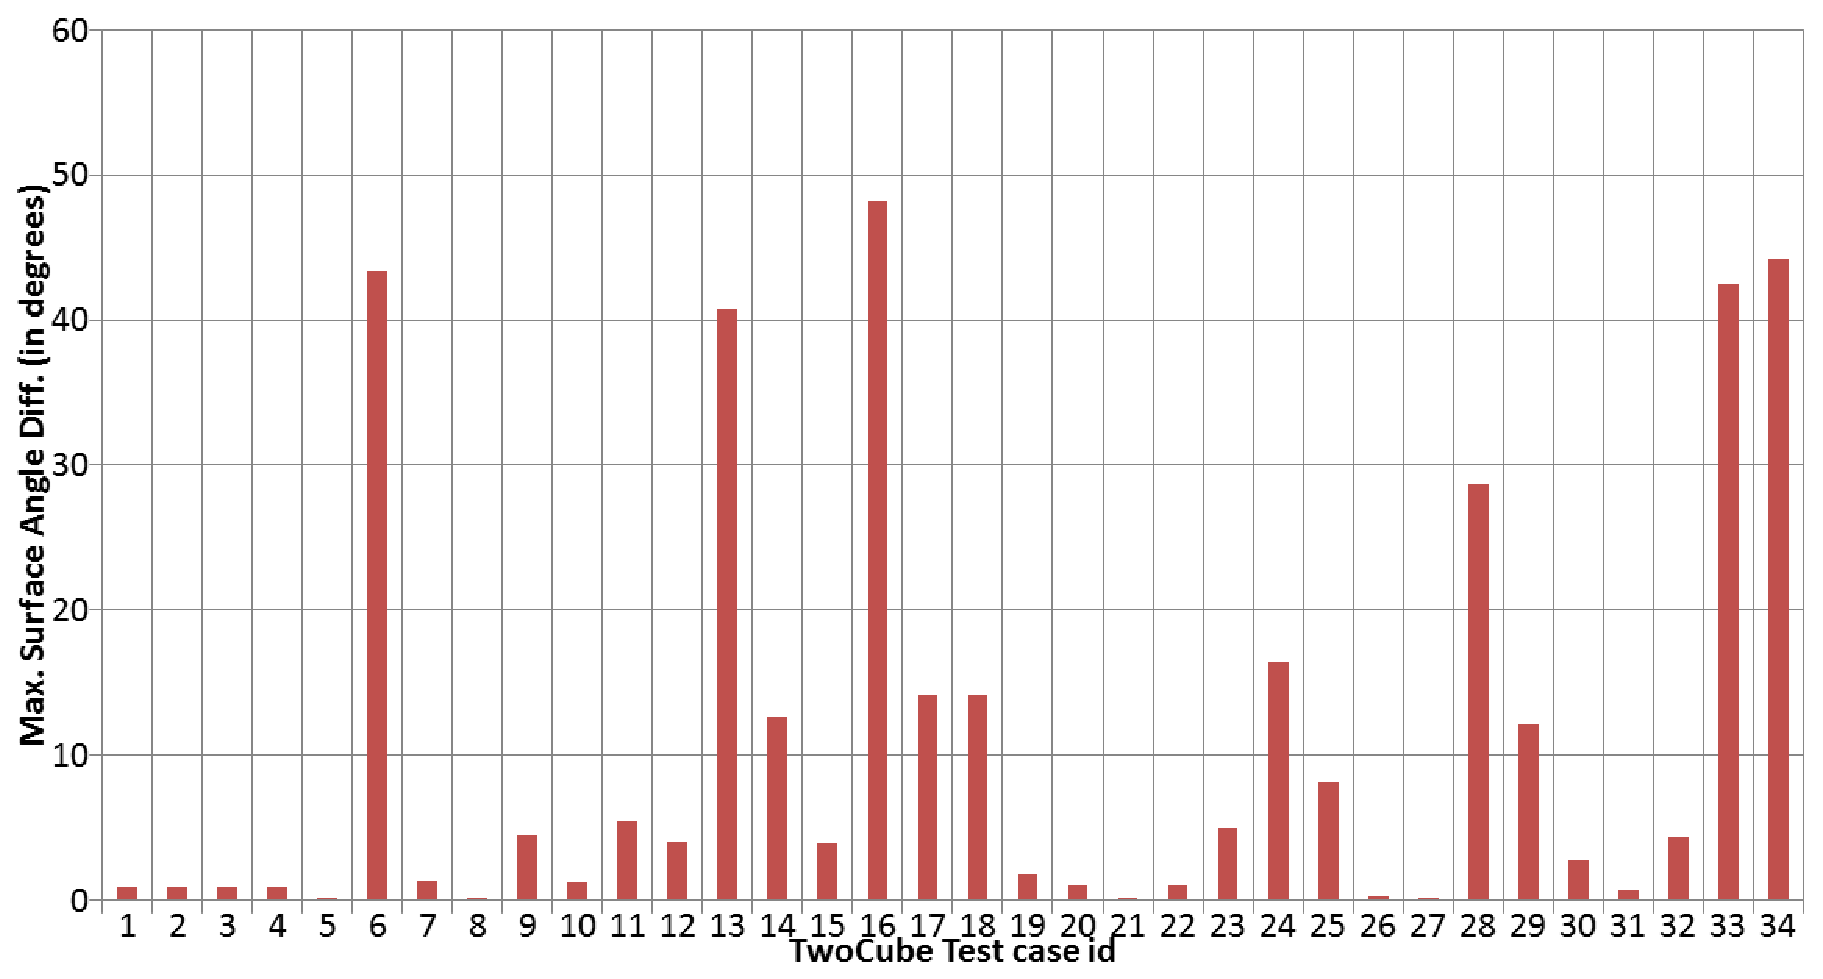
\includegraphics[width=0.45\linewidth]{images/tw2.eps} \\
(a) SHREC using exact gradients & (b) SHREC using Religrad gradients \\
\\
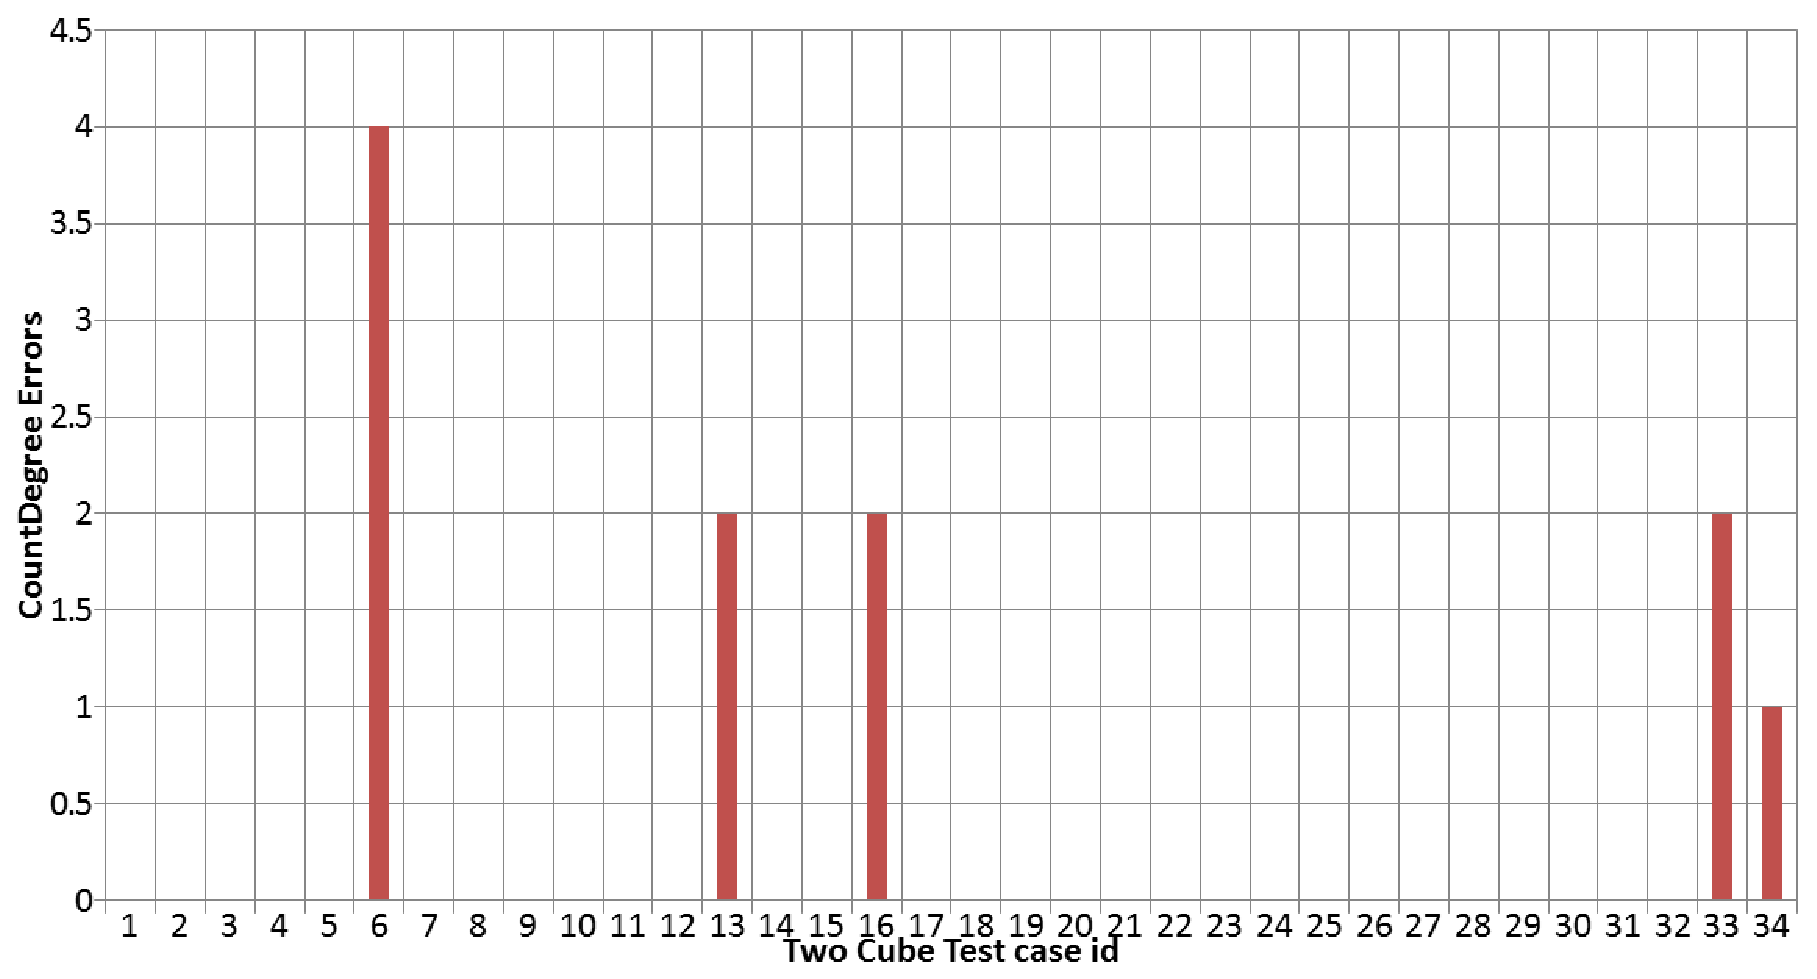
\includegraphics[height=0.25\linewidth]{images/tw3.eps} &
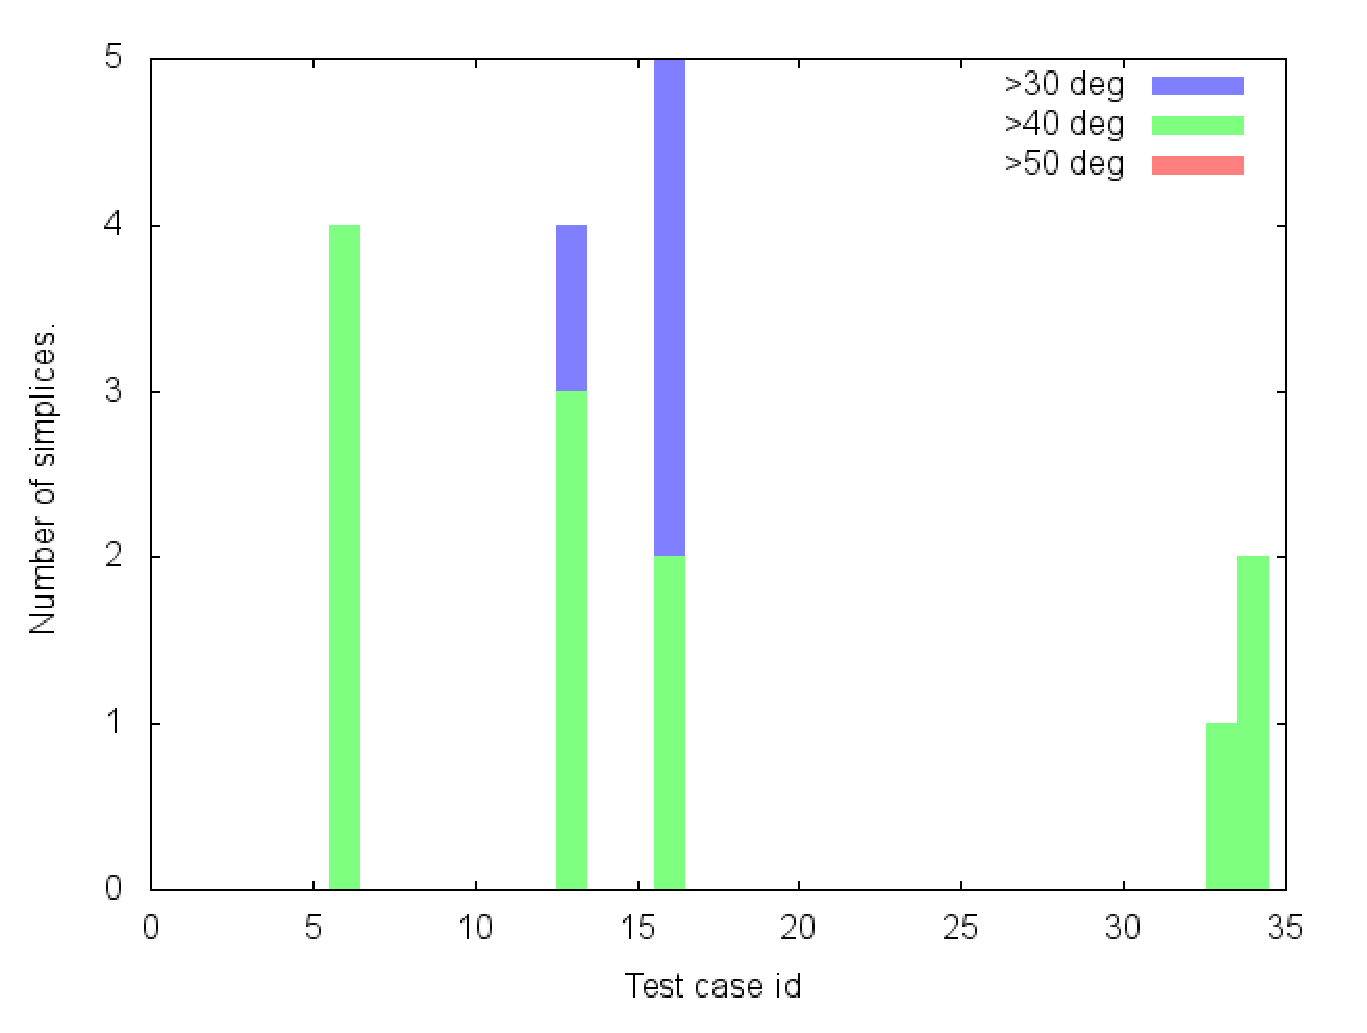
\includegraphics[height=0.25\linewidth]{images/twoCube35_test_1.eps} \\
(c) Shrec using Religrad gradients & (d) SHREC using Religrad Gradients
\end{tabular}

\caption{Results of SHREC using exact and Religrad gradients 
on 34 TwoCubes datasets. 
(a) Unoriented angle distance between isosurface (exact gradients)
and polygonal mesh.
(Note that the $y$-scale is from 0 to $10^\circ$.)
(b) Unoriented angle distance between isosurface (Religrad gradients)
and polygonal mesh.
(c)~Number of isosurface triangles (Religrad gradients)
with angle difference to polygonal mesh above 30, 40, 50 degrees.
(d)~Number of degree errors in the 1-skeleton of sharp edges
(Religrad gradients).
(SHREC using exact gradients produces no degree errors.)}
\label{fig:shrecTwoCube}

\end{figure*}


\subsection{Isosurface Reconstruction on Synthetic Data}
\label{section:synthetic_tests}

We tested SHREC on 40 Flange data sets with 40 different orientations
and 34 TwoCubes data sets with 34 different orientations.
Table~\ref{table:datasets} presents data set sizes, isovalues,
and average isosurface sizes.
We tested SHREC both on gradients produced by exact formulas 
and on gradients produced by ReliGrad.
We measured the unoriented angle distance between the SHREC isosurfaces
and the polygonal meshes representing the level sets.
We also counted the number of isosurface triangles whose normal differences
were above $30^\circ$, $40^\circ$ and $50^\circ$.
Finally, we measured the number of degree errors 
in the 1-skeleton of sharp isosurface edges.

Figure~\ref{fig:flange1} shows a Flange isosurface produced by SHREC
using exact gradients.
The magnified region shows edges with dihedral angle
less than $140^\circ$ in red blended with a subset of the ``non-sharp"
edges.

With exact gradients,
all the Flange isosurfaces had unoriented angle distance
under ??? from the polygonal meshes.
They also had no degree errors in the 1-skeletons
of sharp isosurface edges,
i.e. all the vertices in the 1-skeletons had degree two.

Figure~\ref{fig:flangeAngle} displays angle distance and degree error
information for the 40 Flange isosurfaces
when gradients were produced using Religrad.
As shown in Figure~\subref*{fig:flangeAngle1},
only one isosurface had triangles with angle distance greater than $50^\circ$
and less than half had no triangles with angle distance greater than $40^\circ$.
No isosurfaces had more than 5 triangles with angle distance
greater than $40^\circ$
and no isosurfaces had more than 15 triangles with angle distance greater
than $30^\circ$.

Figure~\subref*{fig:flangeAngle2} displays a histogram of angle distances
for a single Flange isosurface (id 17) 
whose gradients were produced using Religrad.
(Note the logarithmic scale.)
As can be seen,
there are very few triangles with angle distance
greater than $20^\circ$, $30^\circ$ or $40^\circ$.
The isosurface mesh has approximately 133
thousand triangles. 

Figure~\protect\subref*{fig:flangeAngle3} shows the 1-skeleton degree errors
for the 40 Flange isosurfaces when gradients were produced using Religrad.
Thirty two isosurfaces (80$\%$) had no degree errors.
No isosurface had more than eight degree errors.

Figure~\ref{fig:shrecPerfect1} shows a TwoCubes isosurface
and isosurface edges constructed by SHREC.
SHREC reproduces the 0-dimensional features with single mesh vertices
and the 1-dimensional features with a sequence of mesh edges
with dihedral angle $90^\circ$.

Figure~\ref{fig:shrecTwoCube} displays angle distance and degree error
information for the 34 TwoCube isosurfaces produced by SHREC.
Figure~\ref{fig:shrecTwoCube}(a) shows the unoriented angle distance
using exact gradients.
As with the exact gradients in the Flange data sets,
the angle distance is very low (less than $2^\circ$)
for all the isosurfaces.)
With exact gradients, the 34 TwoCubes isosurfaces 
had no 1-skeleton degree errors, 
i.e. they all had exactly 20 vertices with degree three 
in the 1-skeleton of their sharp edges.

Figure~\ref{fig:shrecTwoCube}(b) shows the unoriented angle distances
using gradients produced by Religrad.
For most isosurfaces, the angle distance is still low (under $10^\circ$),
although six isosurfaces have angle distances of between $30^\circ$
and $50^\circ$.
The high angle distances indicate errors in the SHREC reconstruction 
of sharp features.

For the isosurfaces constructed using Religrad gradients,
Figure~\ref{fig:shrecTwoCube}(c) gives
the number of isosurface triangles whose normal differences
are above $30^\circ$, $40^\circ$ and $50^\circ$.
Dataset 16, which had the largest angle distance over all 34 isosurfaces,
has only 5 triangles with normal difference more than 30$^\circ$ 
and a single triangle with normal distance over 40$^\circ$.  

Figure~\ref{fig:shrecTwoCube}(d) shows
the degree errors in the 1-skeleton of sharp edges
when gradients were produced using Religrad.
29 out of the 34 TwoCubes isosurfaces had no degree errors.
Of the 5 isosurfaces with degree errors,
the maximum number of degree errors was four.
As previously noted,
there were no degree errors for any of the 34 TwoCubes isosurfaces
when SHREC used exact gradients.

\begin{figure}[t]
	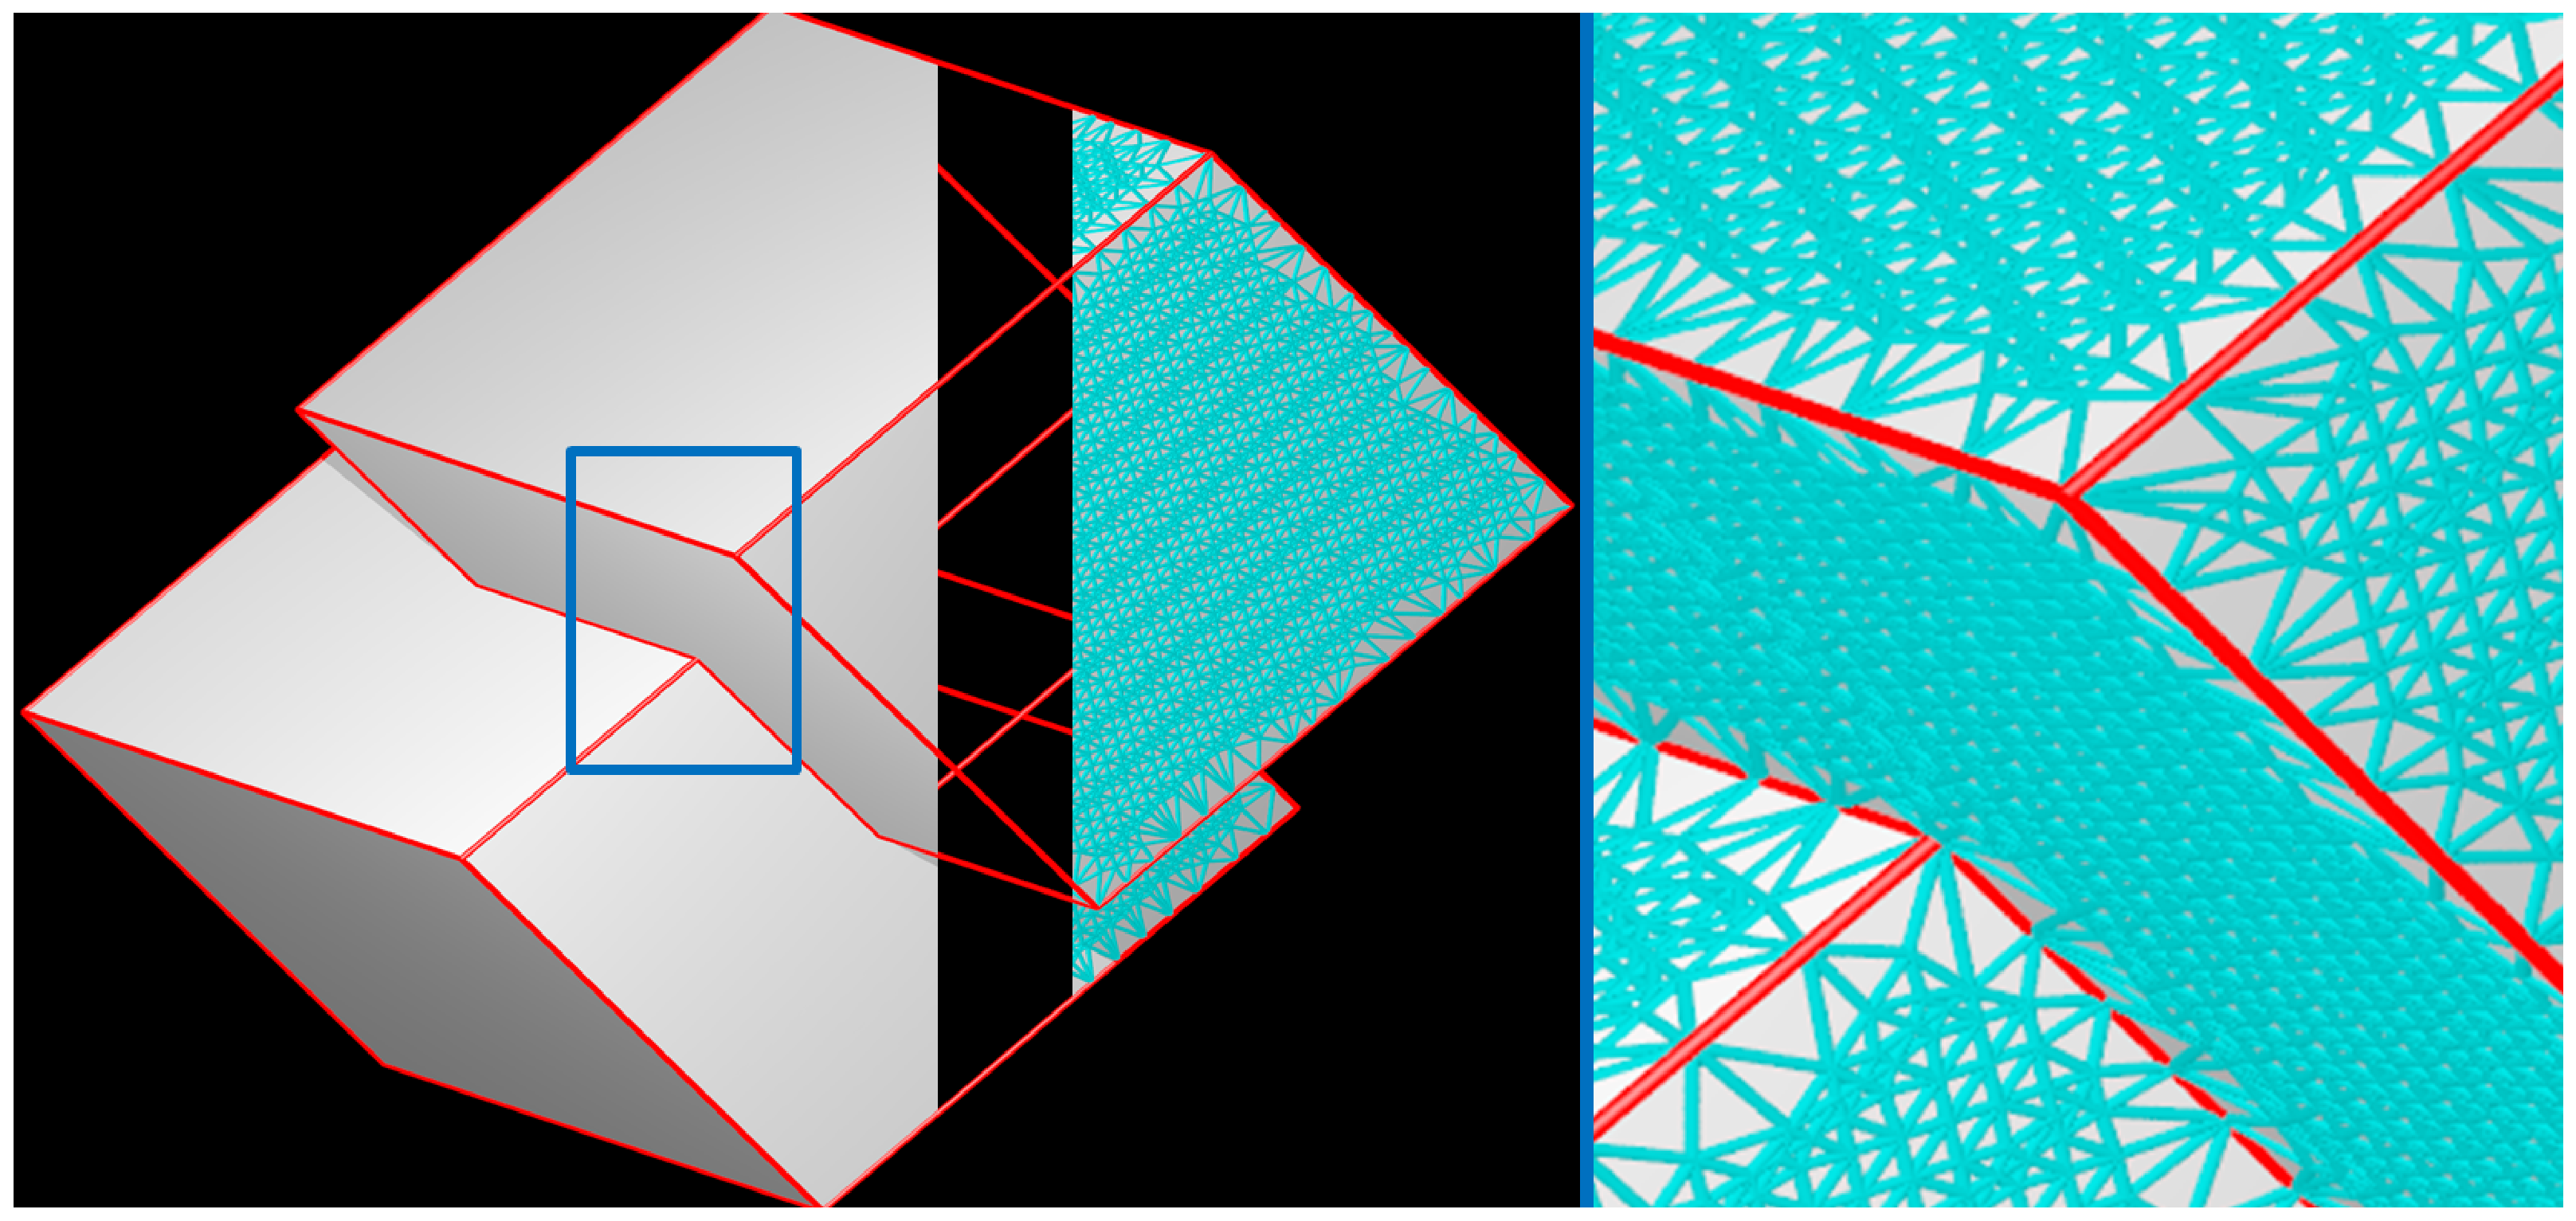
\includegraphics[width=\linewidth]{images/shrecPerfect.eps}
	\caption{SHREC TwoCubes isosurface. 
``Sharp" edges (dihedral angle less than $140^\circ$) are marked in red. 
Smooth edges are shown in cyan. The magnified region shows the output mesh edges around a corner.}
	\label{fig:shrecPerfect1}
\end{figure}

\begin{figure}[t]
\subfloat[Cannon]{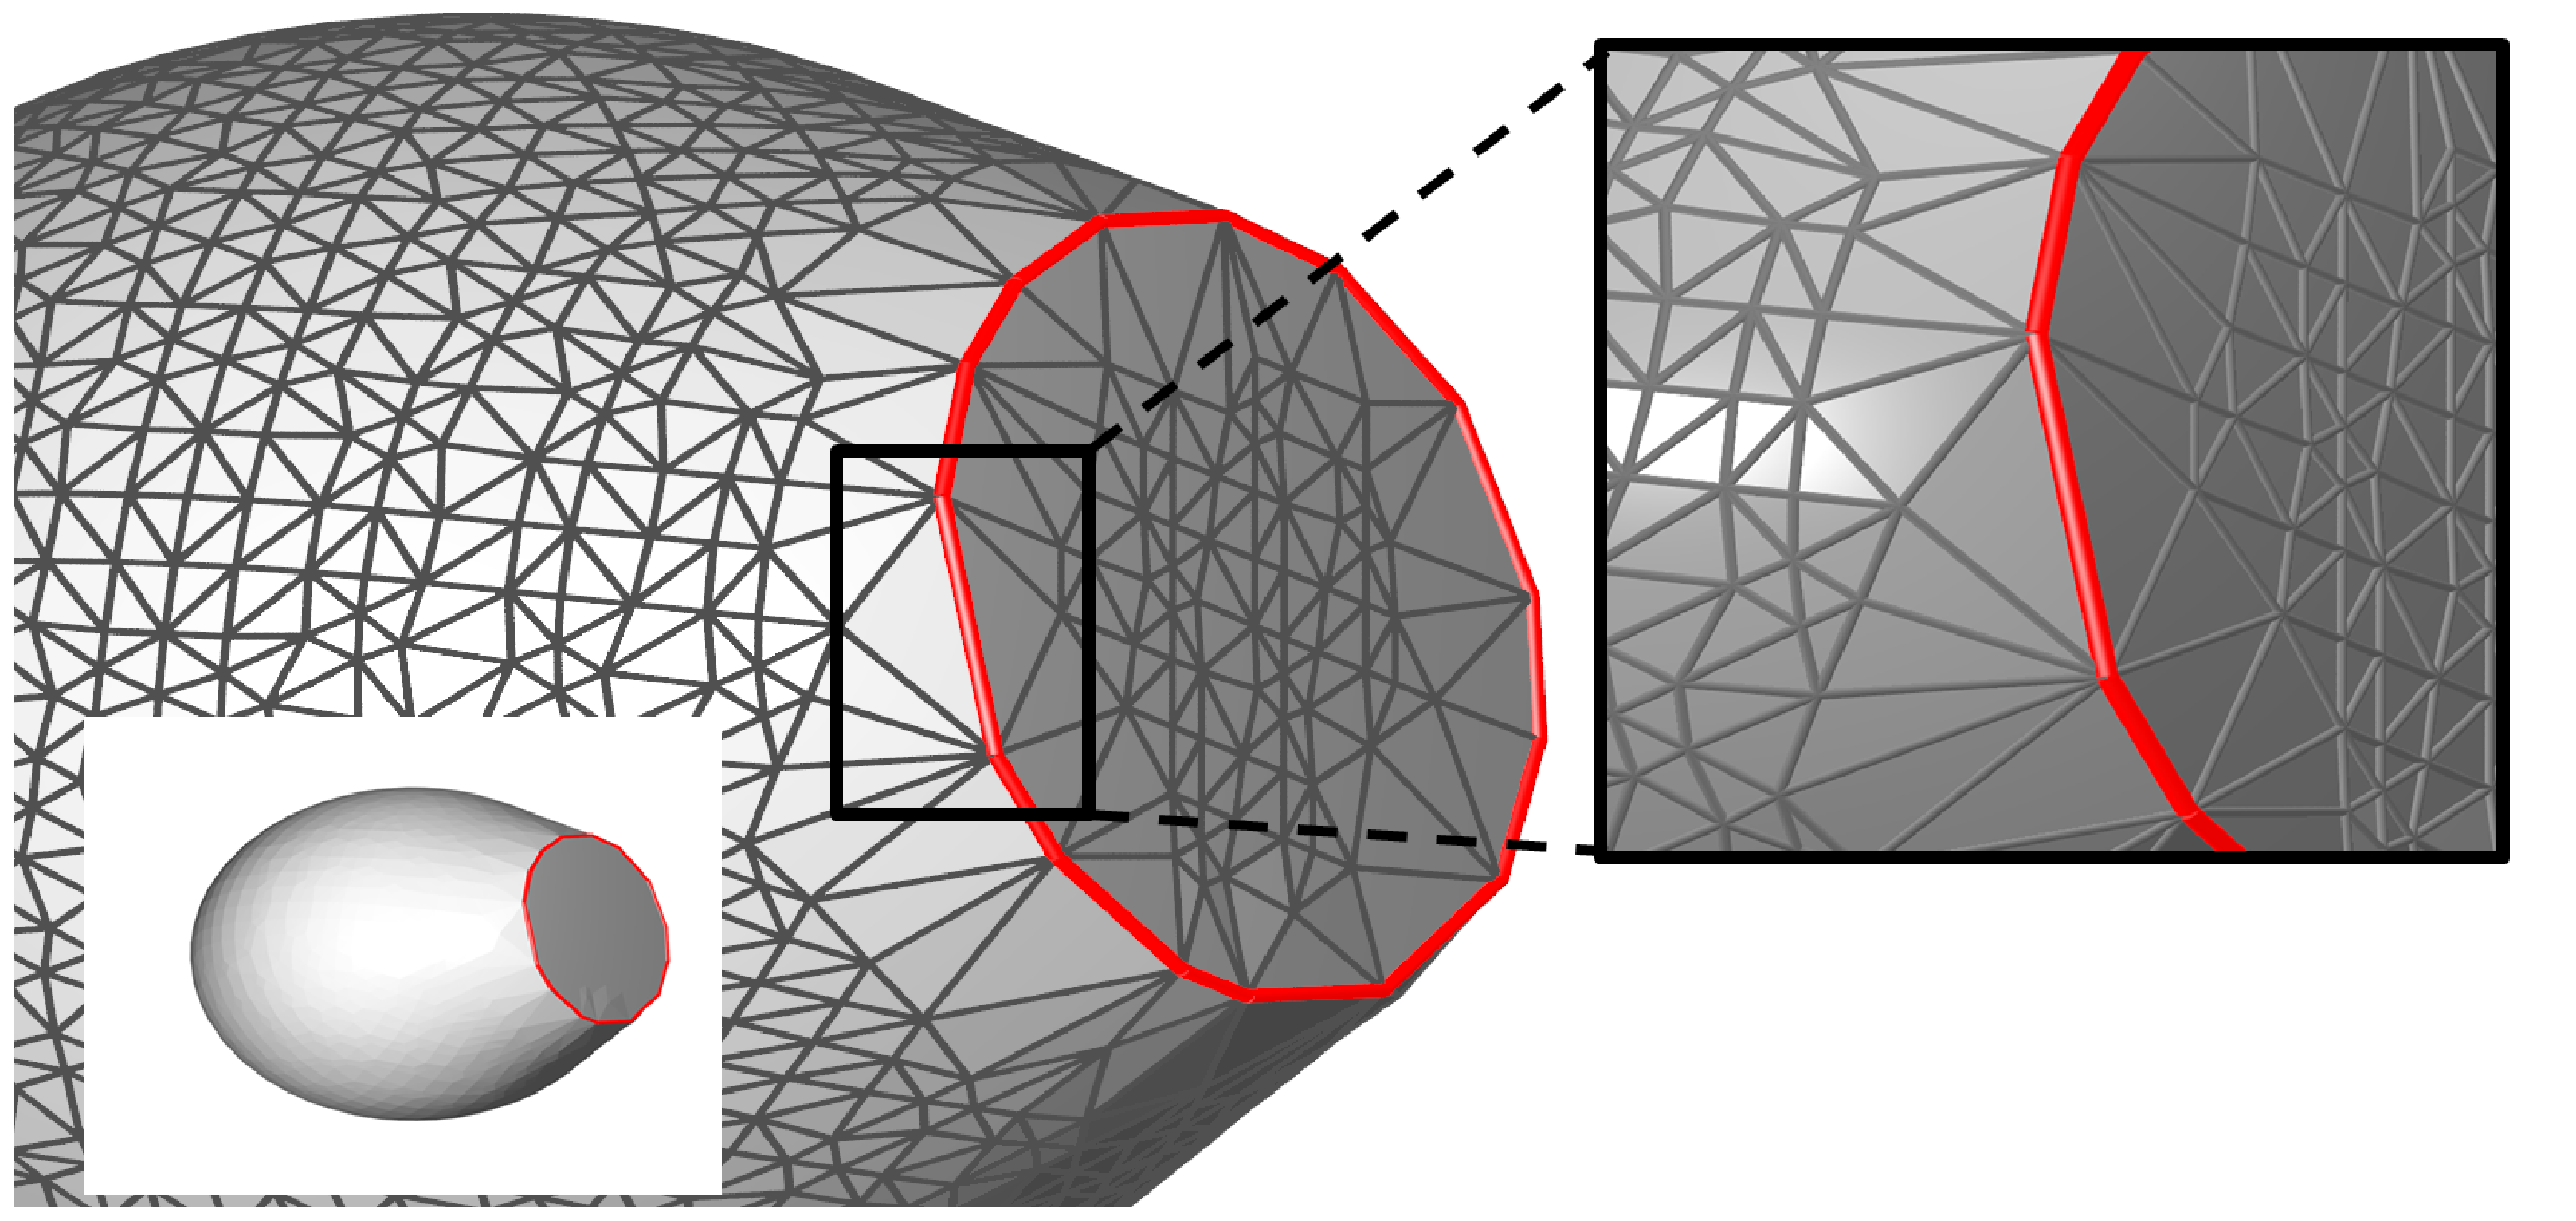
\includegraphics[width=0.5\linewidth]{images/cannon2.eps}\label{fig:cannon:a}}
\subfloat[Smooth Tip Cone]{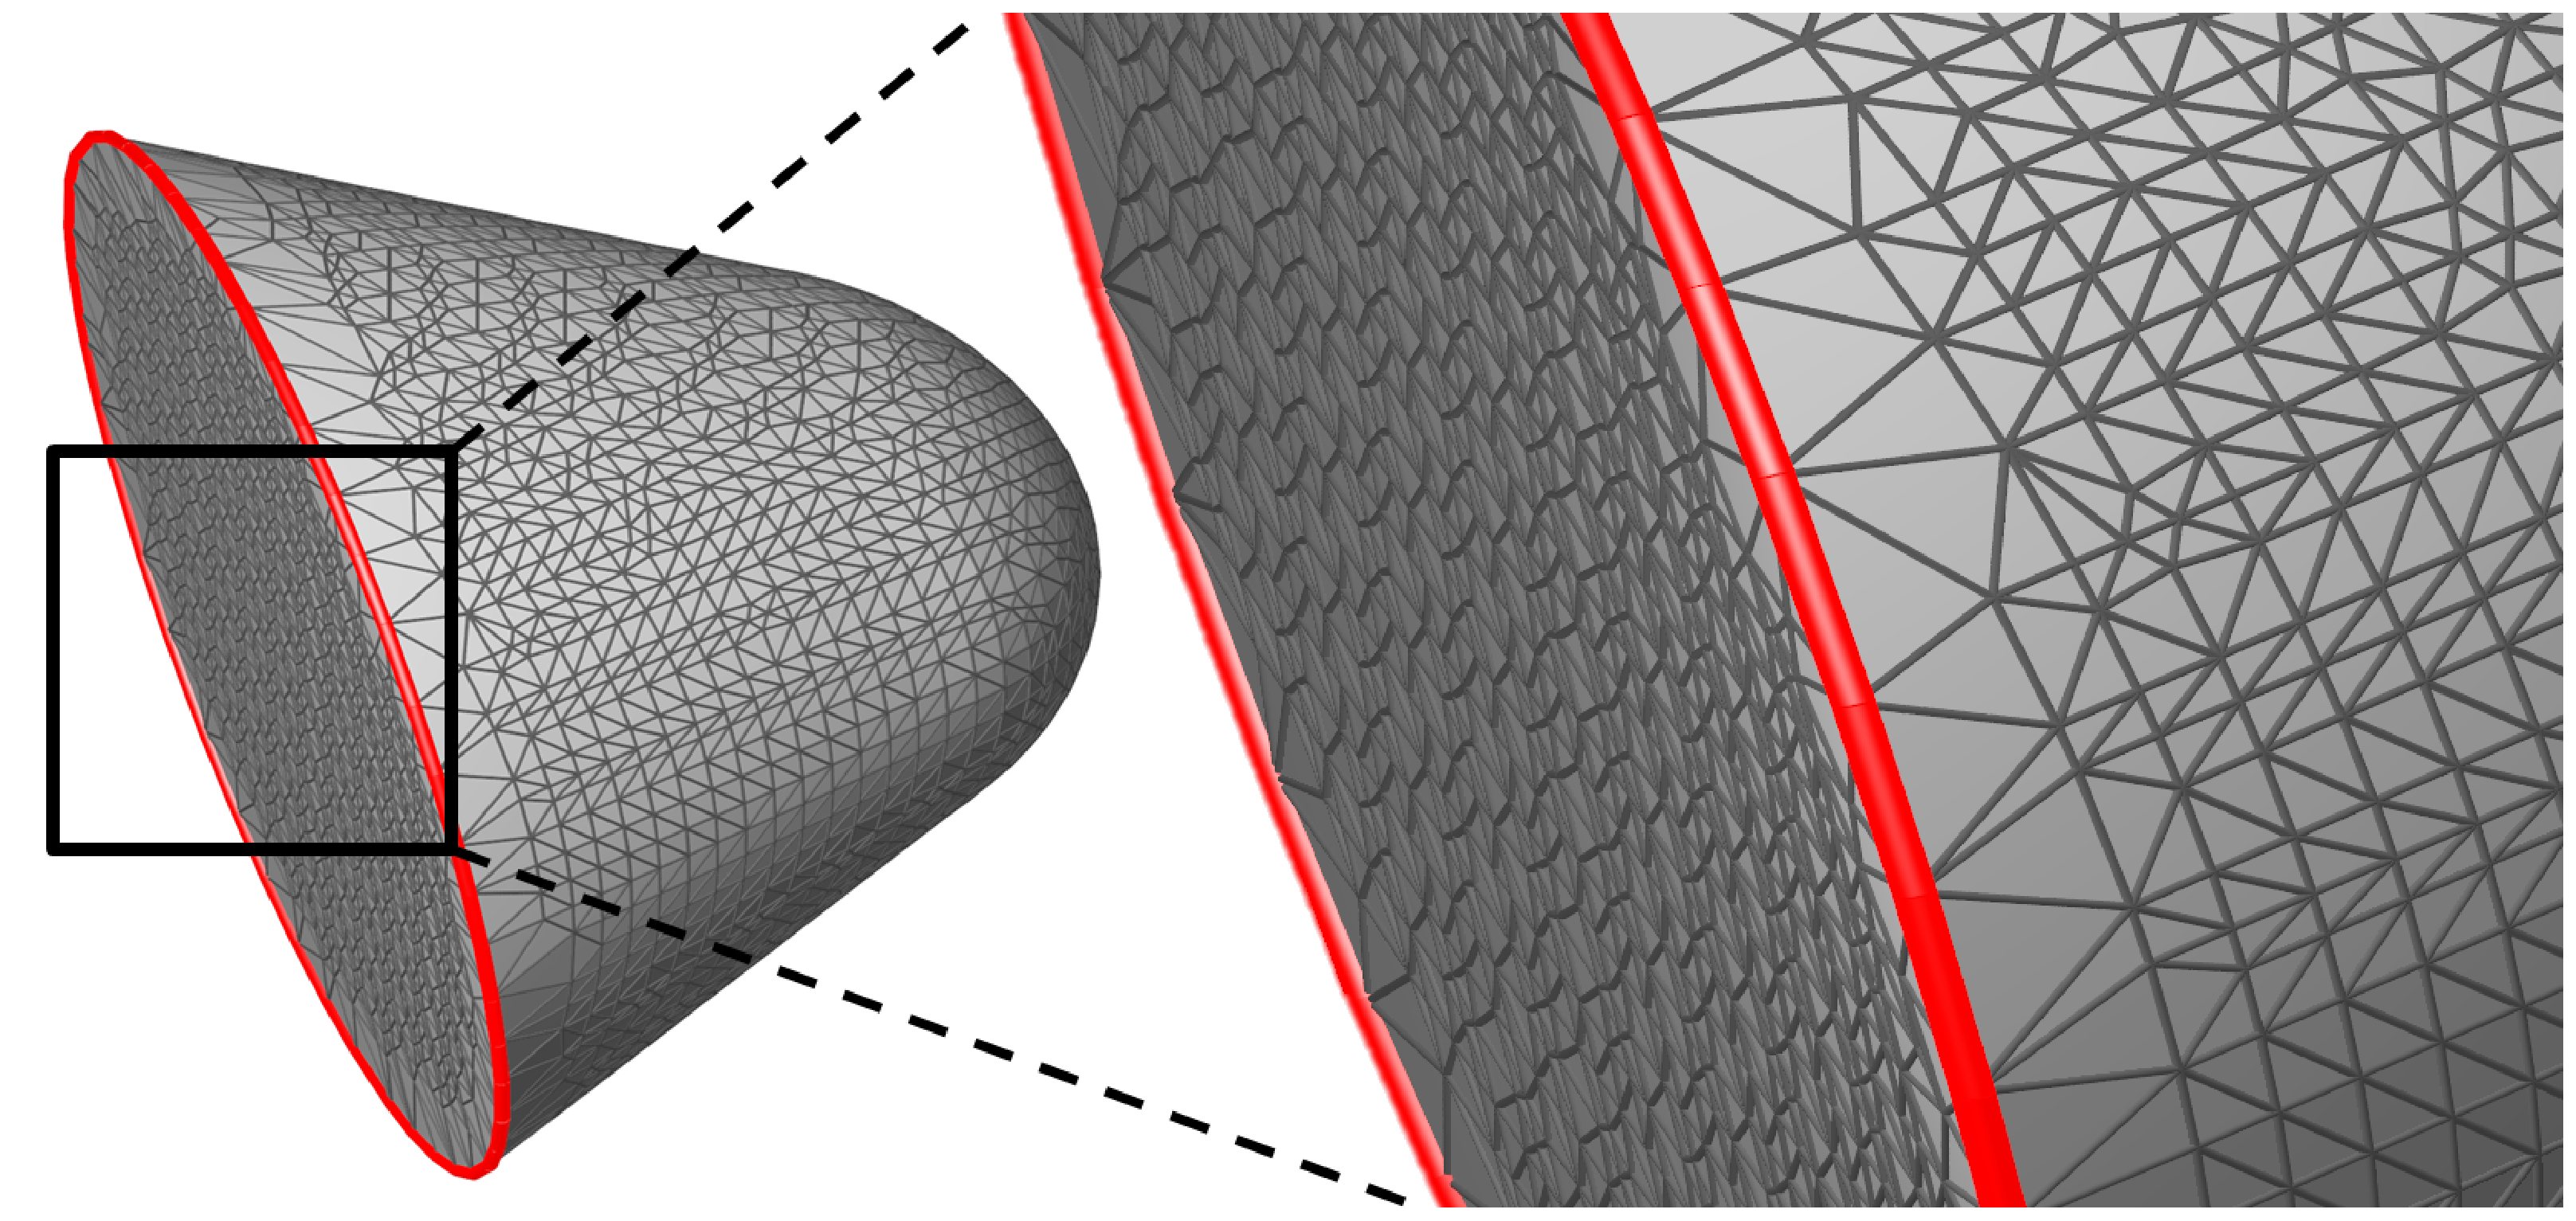
\includegraphics[width=0.5\linewidth]{images/cone2.eps}\label{fig:cone:a}}
\caption{SHREC Cannon and Smooth Tip Cone isosurfaces (Religrad gradients.) 
(a)~Cannon isosurface.
\mbox{1-dimensional} feature has dihedral angle $120^\circ$.
(b)~Smooth Tip Cone isosurface.  1-dimensional feature has dihedral angle $60^\circ$.}
\label{fig:cannon_cone}
\end{figure}

\begin{figure}[t]
	\subfloat[]{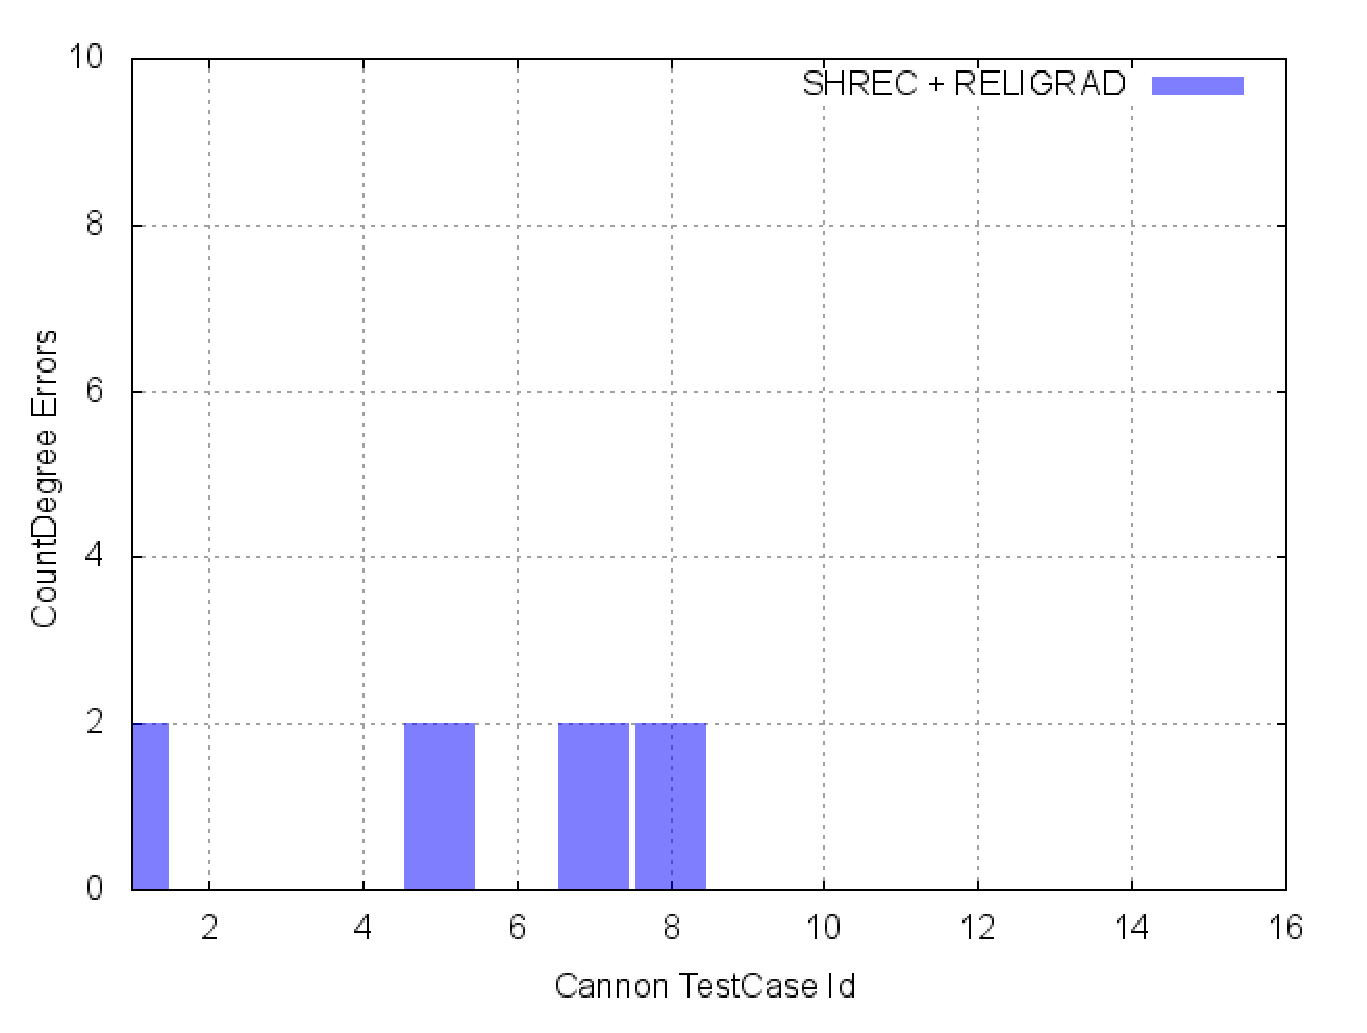
\includegraphics[width=0.5\linewidth]{images/cannon.eps}\label{fig:cannon:b}}
	\subfloat[]{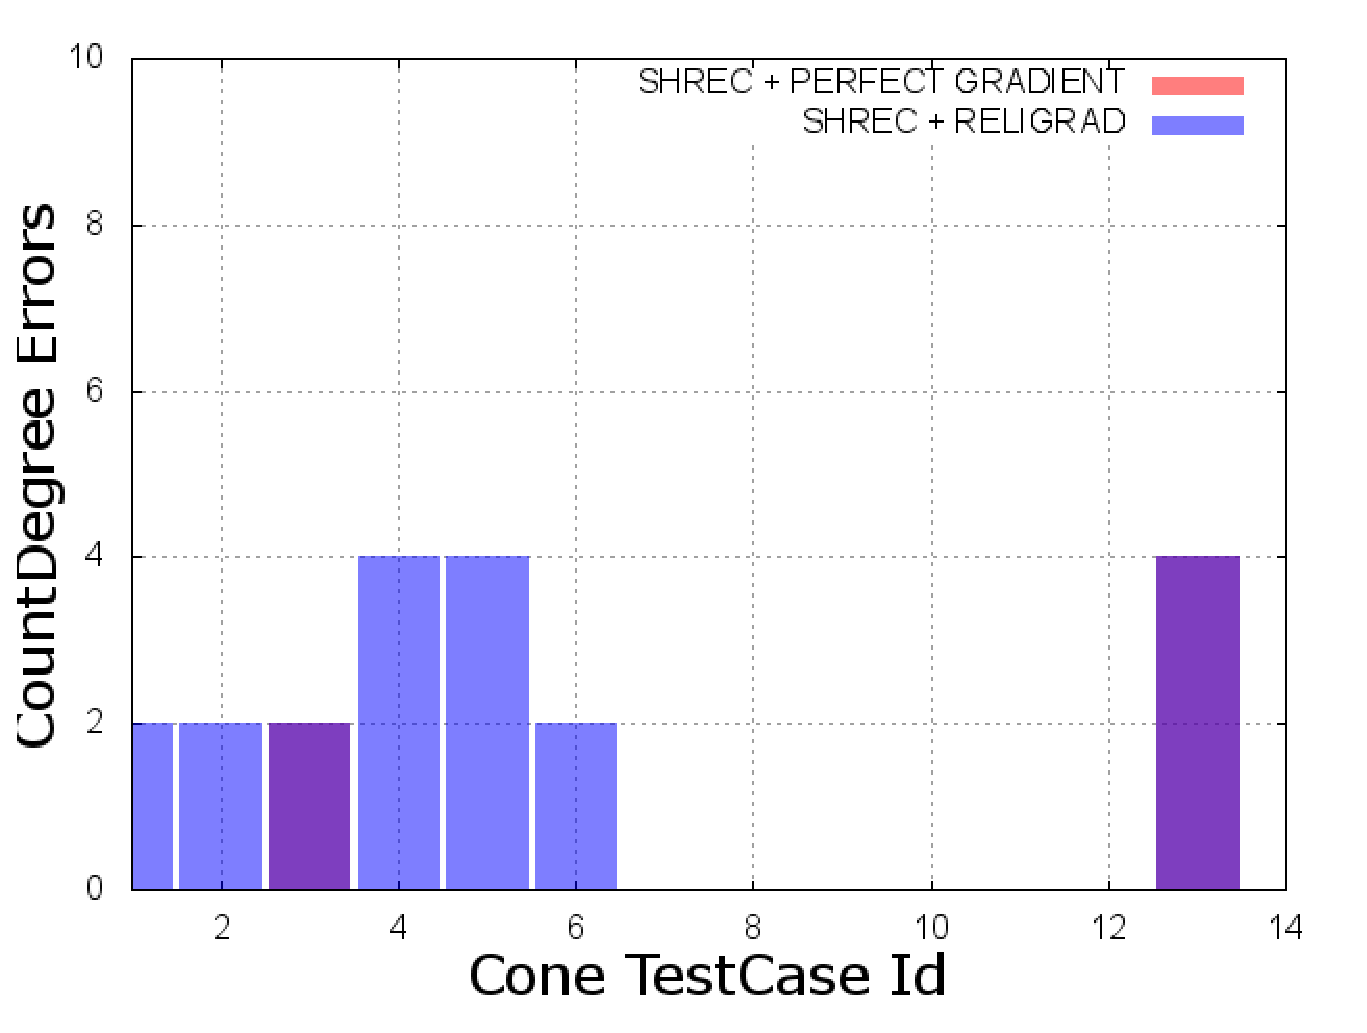
\includegraphics[width=0.5\linewidth]{images/cone.eps}\label{fig:cone:b}}

\caption{Results of SHREC on 15 Cannon and 14 Smooth Tip Cone data sets.
(a) Number of degree errors on 1-skeleton of Cannon isosurfaces
constructed using Religrad gradients.
(Cannon isosurfaces constructed using exact gradients had no degree errors.)
(b) Number of degree errors on 1-skeleton of Smooth Tip Cone isosurfaces
constructed using Religrad gradients (green) and exact gradients 
(red, labelled SHREC+SYNTHETIC GRADIENTS).}
\label{fig:cannon_cone_summary}
\end{figure}

To measure the dihedral angles other than $90^\circ$,
we ran SHREC on 15 Cannon data sets with 15 different orientations
and 14 Smooth Tip Cone data sets with 14 different orientations.
The 1-dimensional features in the Cannon level sets
had dihedral angles of $60^\circ$.
The 1-dimensional features in the Smooth Tip Cone level sets
had dihedral angles of $120^\circ$.
As expected, SHREC produced more errors than on the Flange or TwoCube
data sets, although it still did quite well.

Figure~\ref{fig:cannon_cone} shows Cannon and Smooth Tip Cone isosurfaces
produced by SHREC using Religrad gradients.
In each, the 1-dimensional is represented by a sequence 
of isosurface mesh edges with the appropriate dihedral angles.

Figure~\ref{fig:cannon_cone_summary} gives the number of degree errors
in the 1-skeleton of sharp edges
for Cannon and Smooth Tip Cone isosurfaces.
SHREC using exact gradients produced no degree errors 
on the 15 Cannon data sets.
SHREC using Religrad produced degree errors on only four Cannon data sets.
For each data set, there were exactly two degree errors.
SHREC using exact gradients produced degree errors in only two 
of the Smooth Tip Cone data sets,
one with two errors and one with four.
SHREC using Religrad gradients produced degree errors on 7 out of the 14
Smooth Tip Cone data sets.
The maximum number of degree errors in any Smooth Tip Cone isosurface
was 4.

\begin{table*}[t]
\centering
\begin{tabular}{|l|l|l|c|}
\hline
Software & Algorithm & URL & References \\
\hline
EMC (IsoEx) & Extended Marching Cubes &
\href{https://www.graphics.rwth-aachen.de/software}{www.graphics.rwth-aachen.de/software} & \cite{kbsh-fssev-01} \\
\hline
EMCpoly & Extended Marching Cubes &
\href{http://web.cse.ohio-state.edu/research/graphics/isotable}{web.cse.ohio-state.edu/research/graphics/isotable} & \\
\hline
PolyMender & Dual Contouring &
\href{http://www.cse.wustl.edu/~taoju/code/polymender.htm}{www.cse.wustl.edu/~taoju/code/polymender.htm} & \cite{j-rrpm-04,jlsw-dchd-02,sw-dcss-02} \\
\hline
SingularCocone & &
\href{http://web.cse.ohio-state.edu/~tamaldey/cocone.html}{web.cse.ohio-state.edu/~tamaldey/cocone.html} & \cite{cdr-drpsc-07,Dey2012} \\
\hline
MergeSharp & &
\href{http://web.cse.ohio-state.edu/research/graphics/isotable}{web.cse.ohio-state.edu/research/graphics/isotable} & \cite{bw-cisec-13,bw-erm-13}\\
\hline
SHREC & &
\href{http://web.cse.ohio-state.edu/research/graphics/isotable}{web.cse.ohio-state.edu/research/graphics/isotable} & \\
\hline
\end{tabular}

\caption{Surface reconstruction software.
EMC is a sample implementation of Extended Marching Cubes.
EMCpoly is a modification of EMC which creates TwoCubes and Flange isosurfaces.
PolyMender is an implementation of dual contouring for fixing polygonal meshes.
SingularCocone is an implementation of a Voronoi based algorithm
for surface reconstruction from point clouds.
The algorithm handles 0 and 1 dimensional features
including non-manifold features.
MergeSharp is an implementation of a dual contouring reconstruction algorithm 
which uses cube merging to obtain better reconstruction around sharp features.
SHREC is an implementation of the algorithm in this paper.}
\label{table:software}
\end{table*}

\begin{figure*}[p]
\centering

\begin{tabular}{cc}
	\subfloat[Flange: Angle distance]{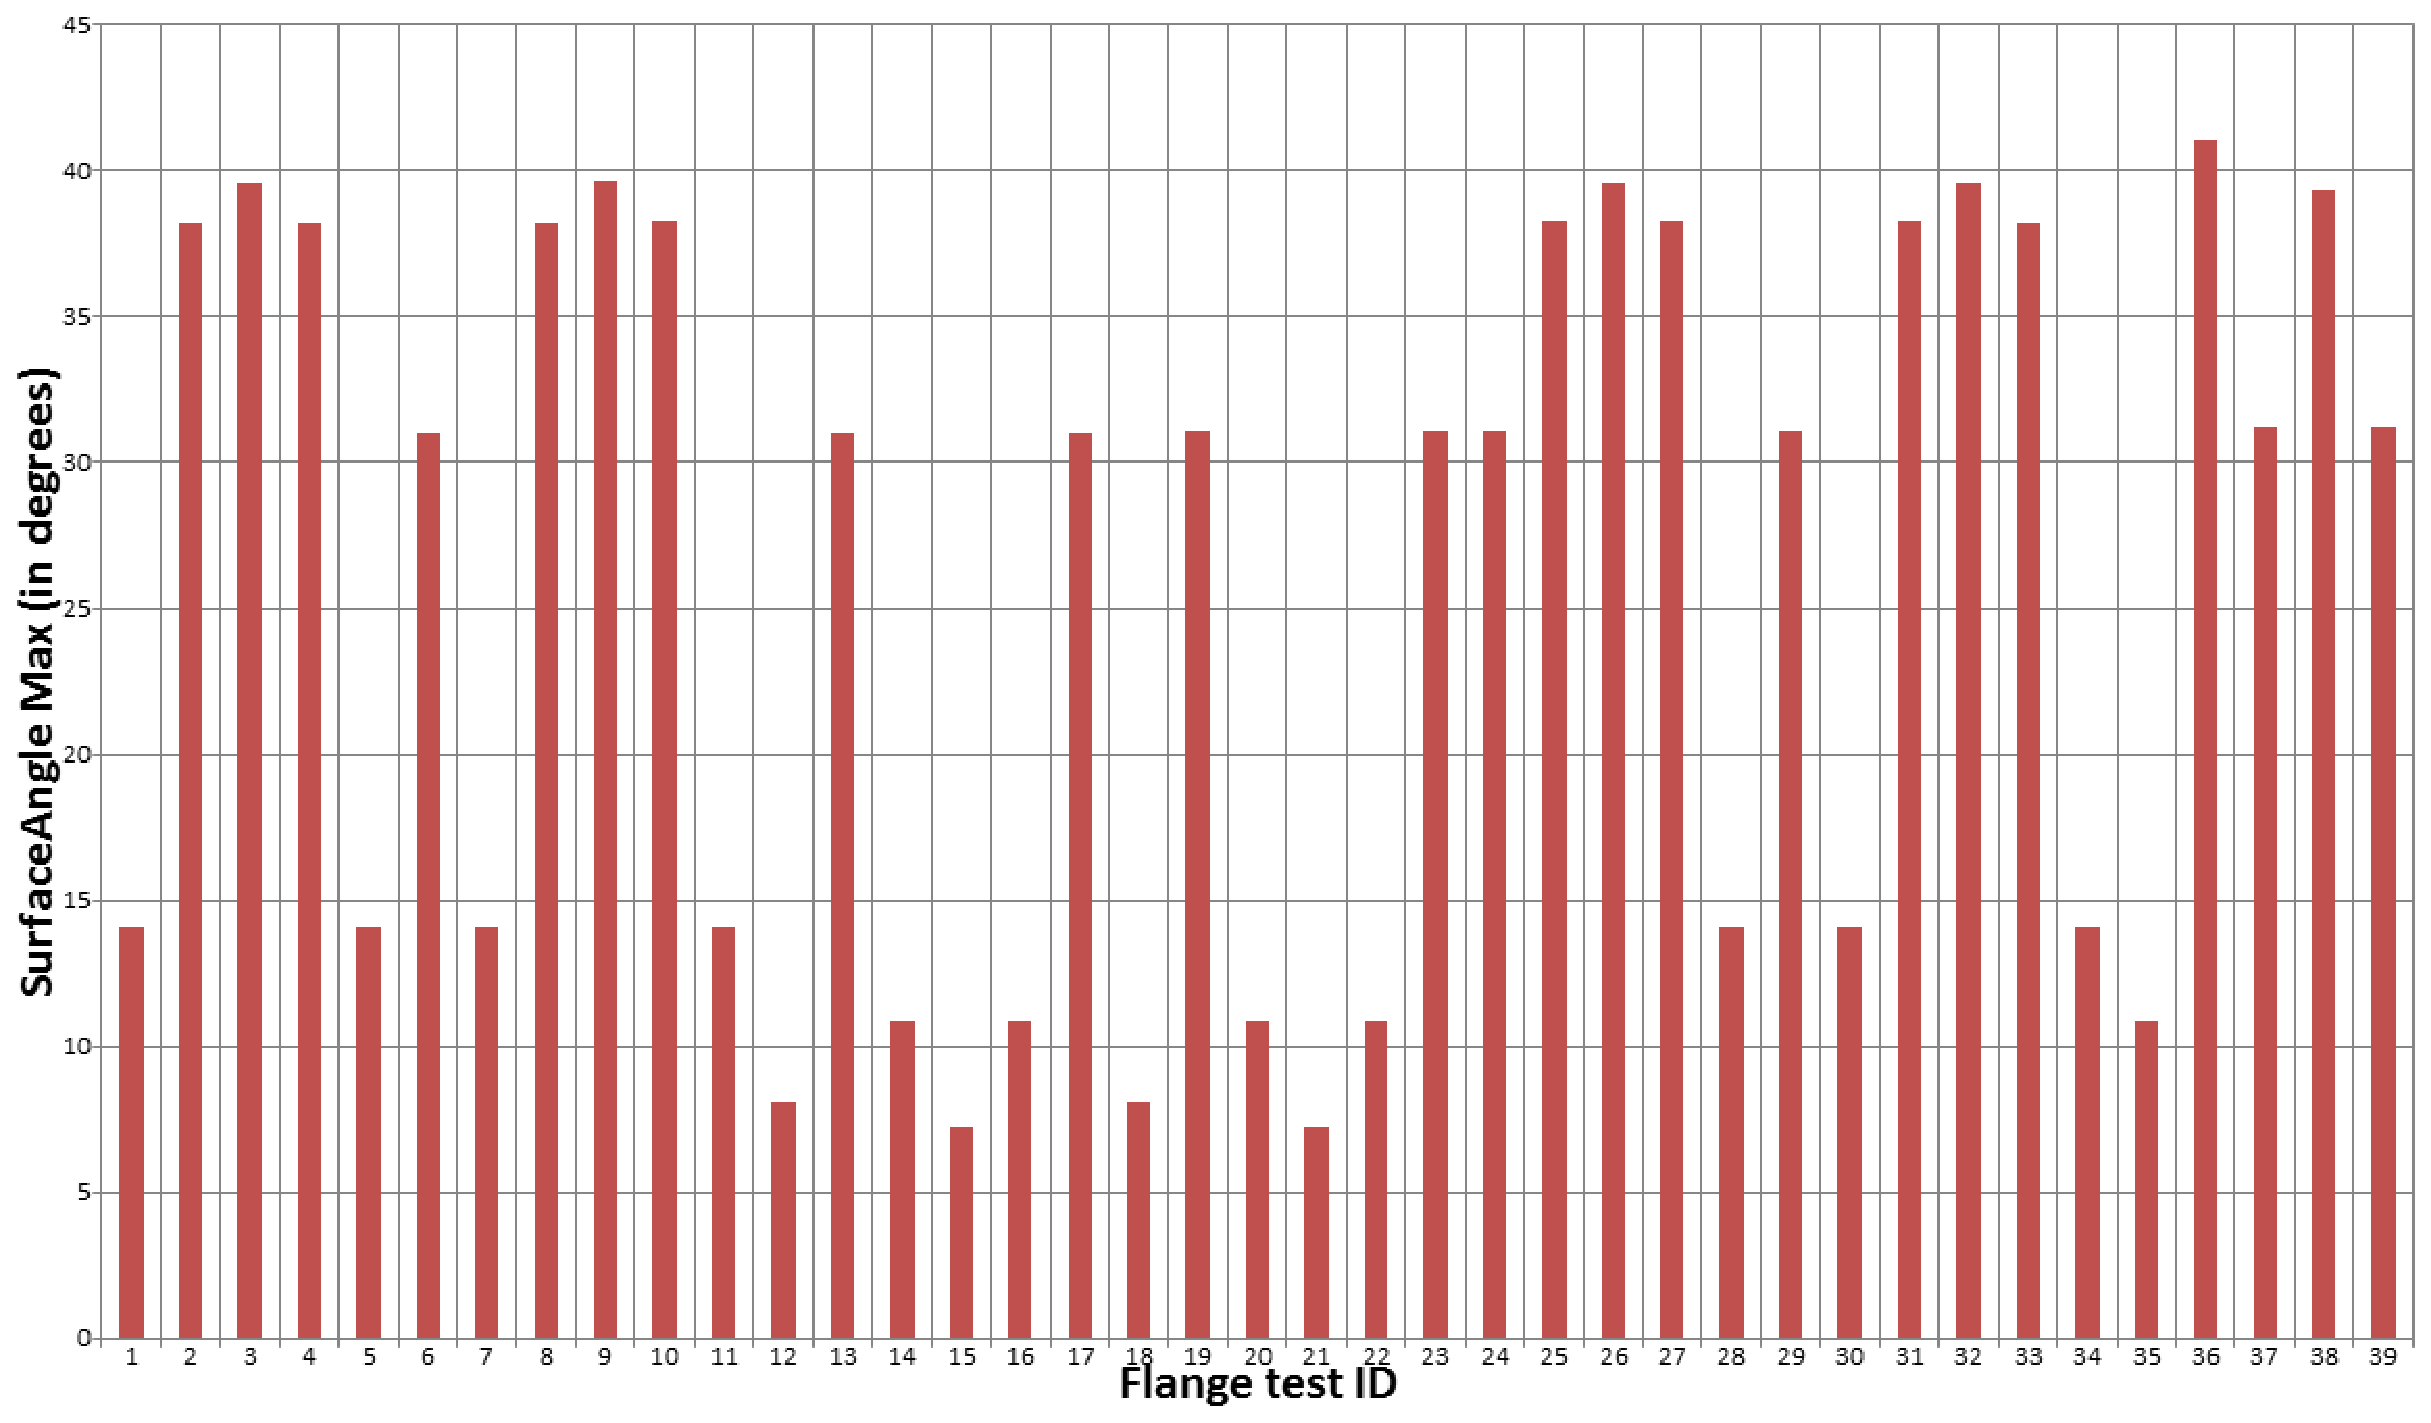
\includegraphics[width=0.45\linewidth]{images/ms_euro_flange_maxAngle.eps}\label{fig:msharp:flange:A}} &
	\subfloat[Flange: Degree errors]{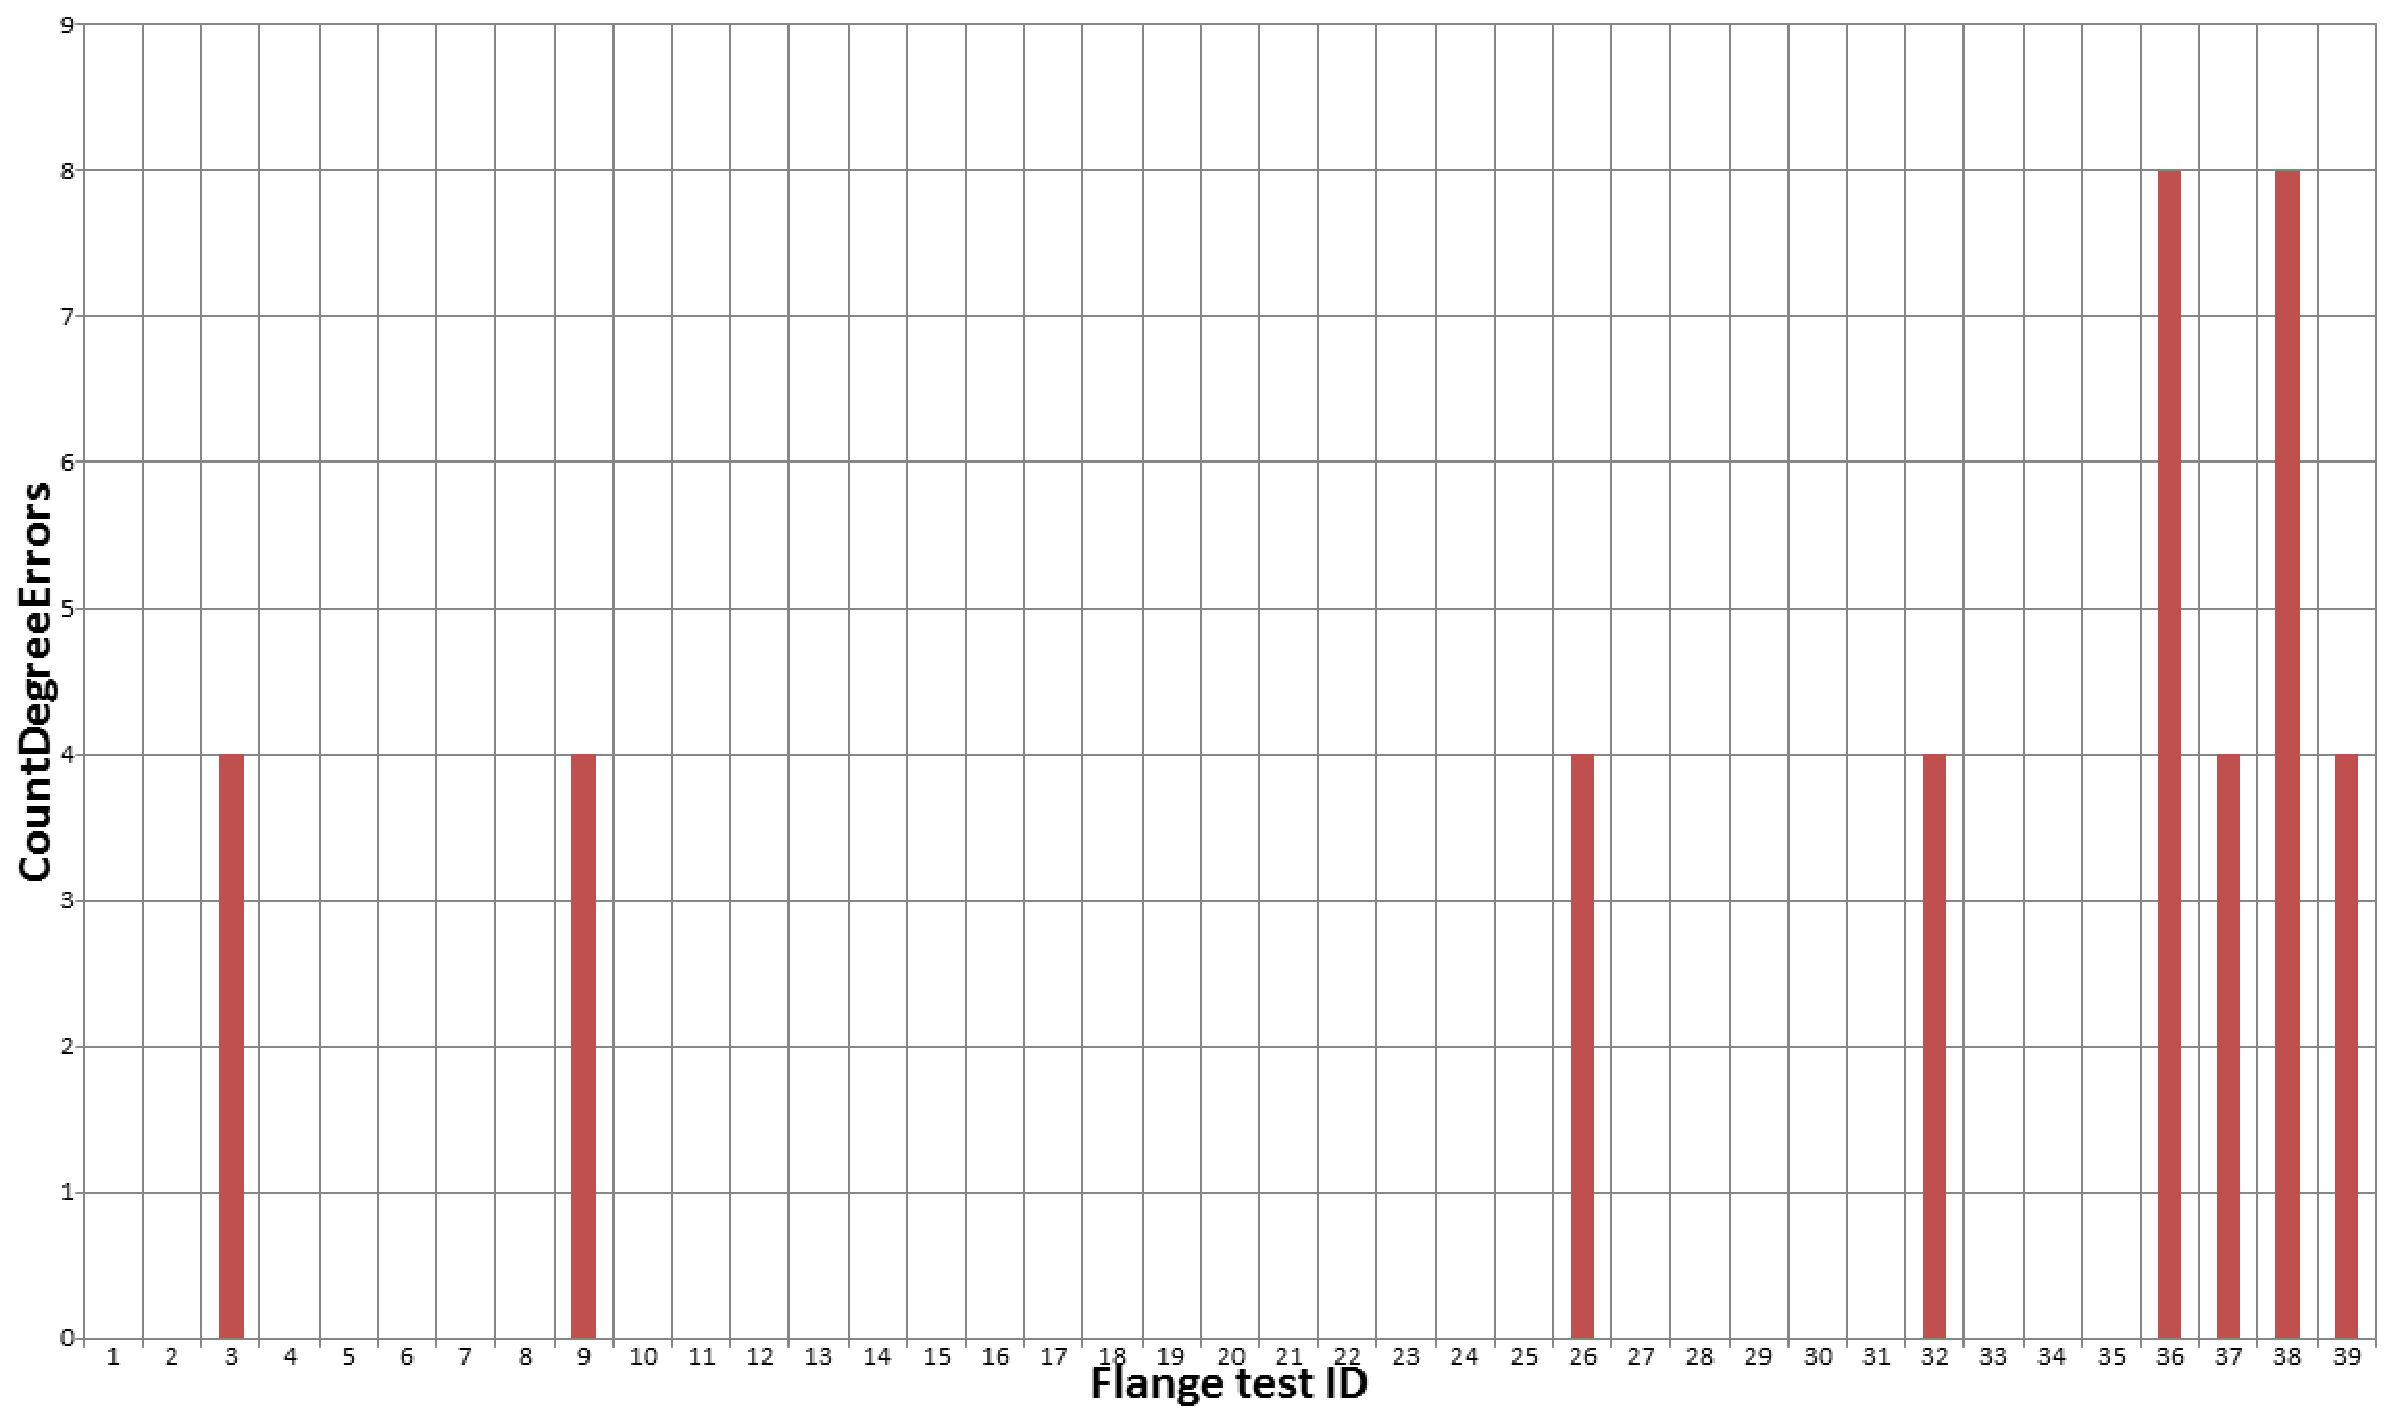
\includegraphics[width=0.45\linewidth]{images/ms_euro_flange_countDegree.eps}\label{fig:msharp:flange:D}} \\
	\subfloat[TwoCubes: Angle distance]{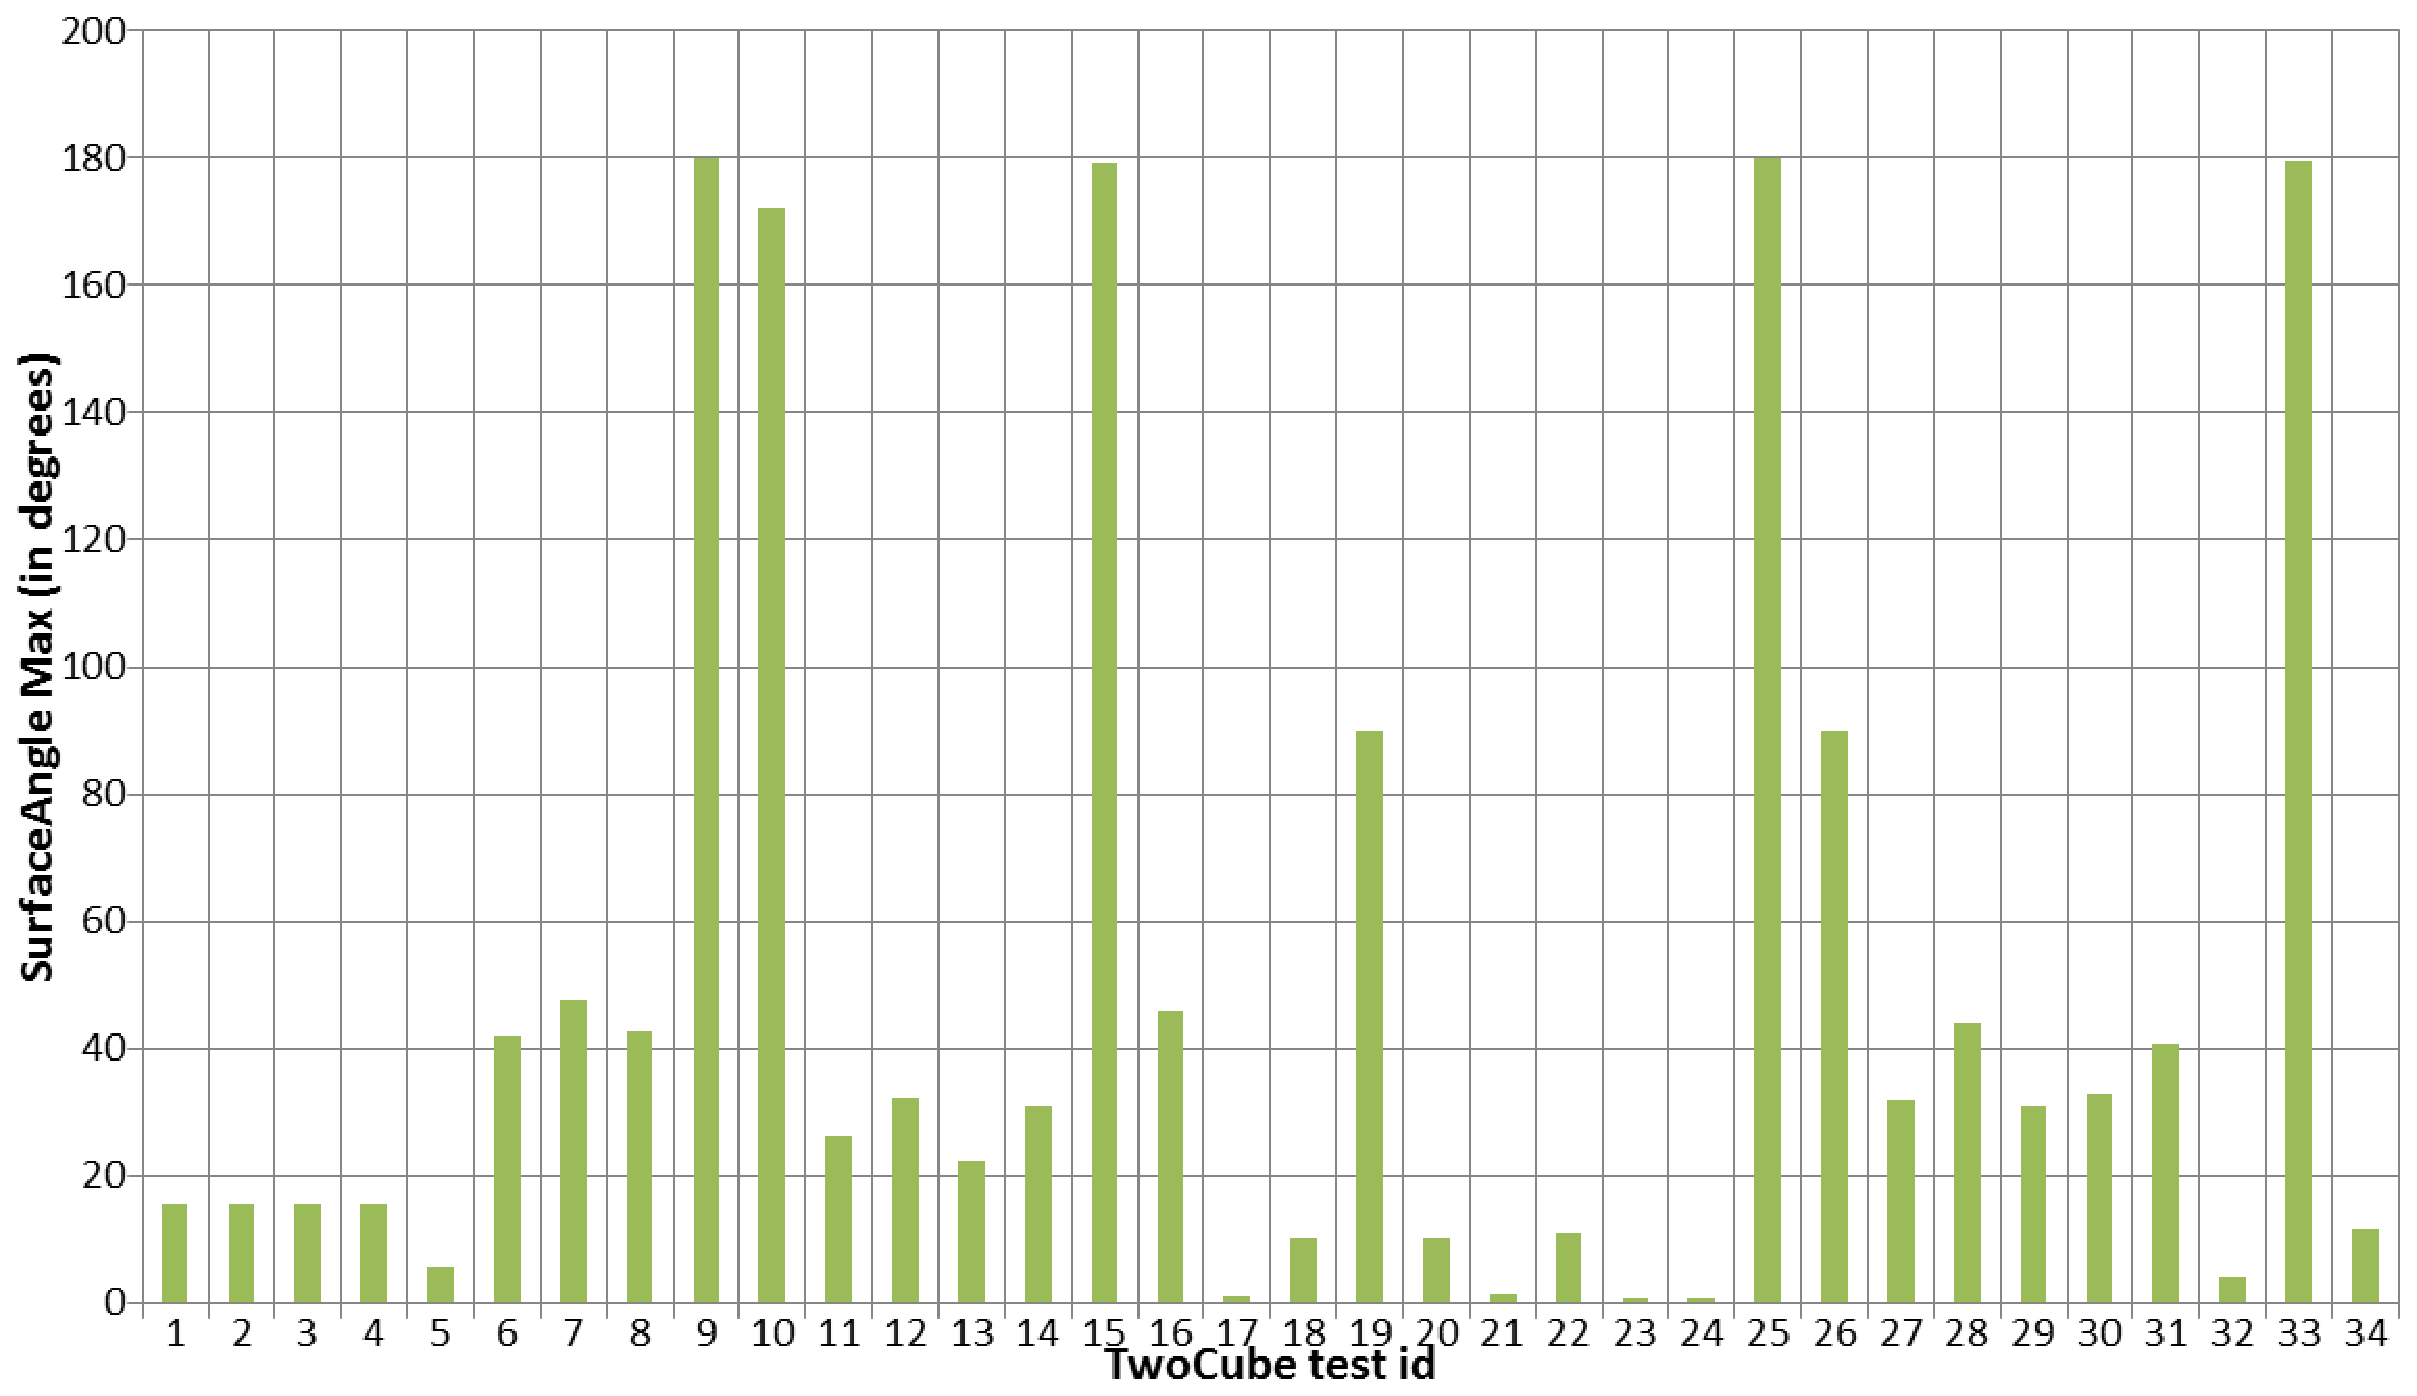
\includegraphics[width=0.45\linewidth]{images/ms_euro_twoCube_maxAngle.eps}\label{fig:msharp:tc:A}} &
	\subfloat[TwoCubes: Degree errors]{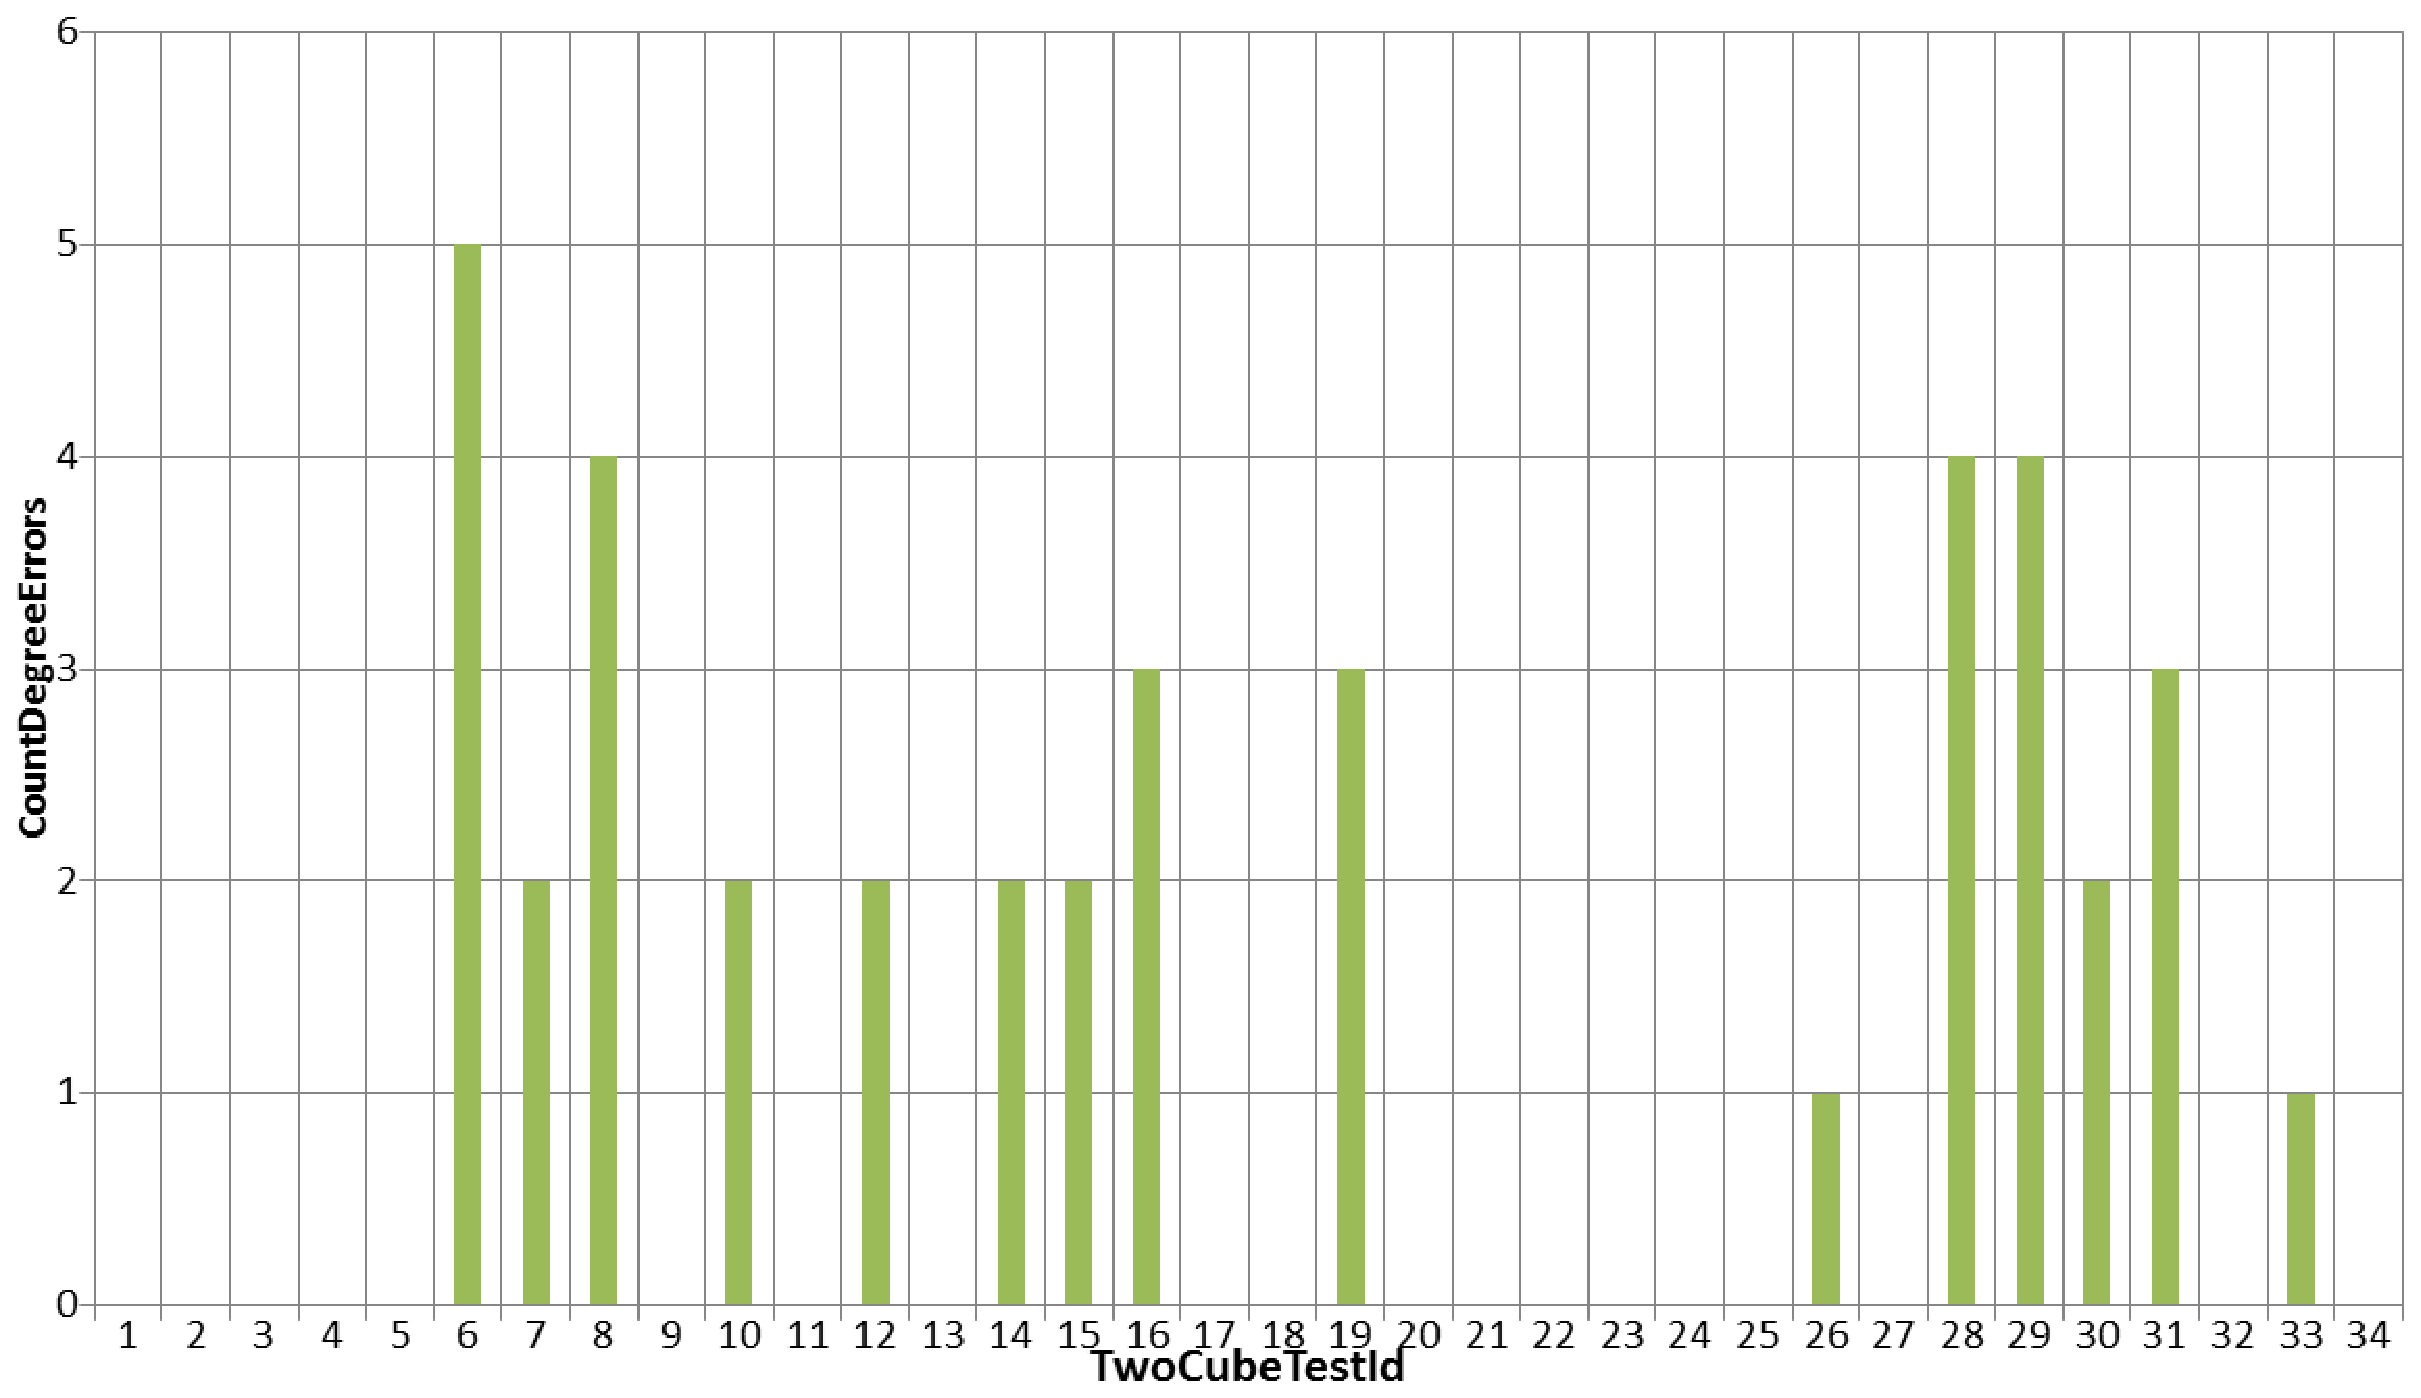
\includegraphics[width=0.45\linewidth]{images/ms_euro_twoCube_countDegree.eps}\label{fig:msharp:tc:D}} \\
	\subfloat[Flange: Triangle normal differences]{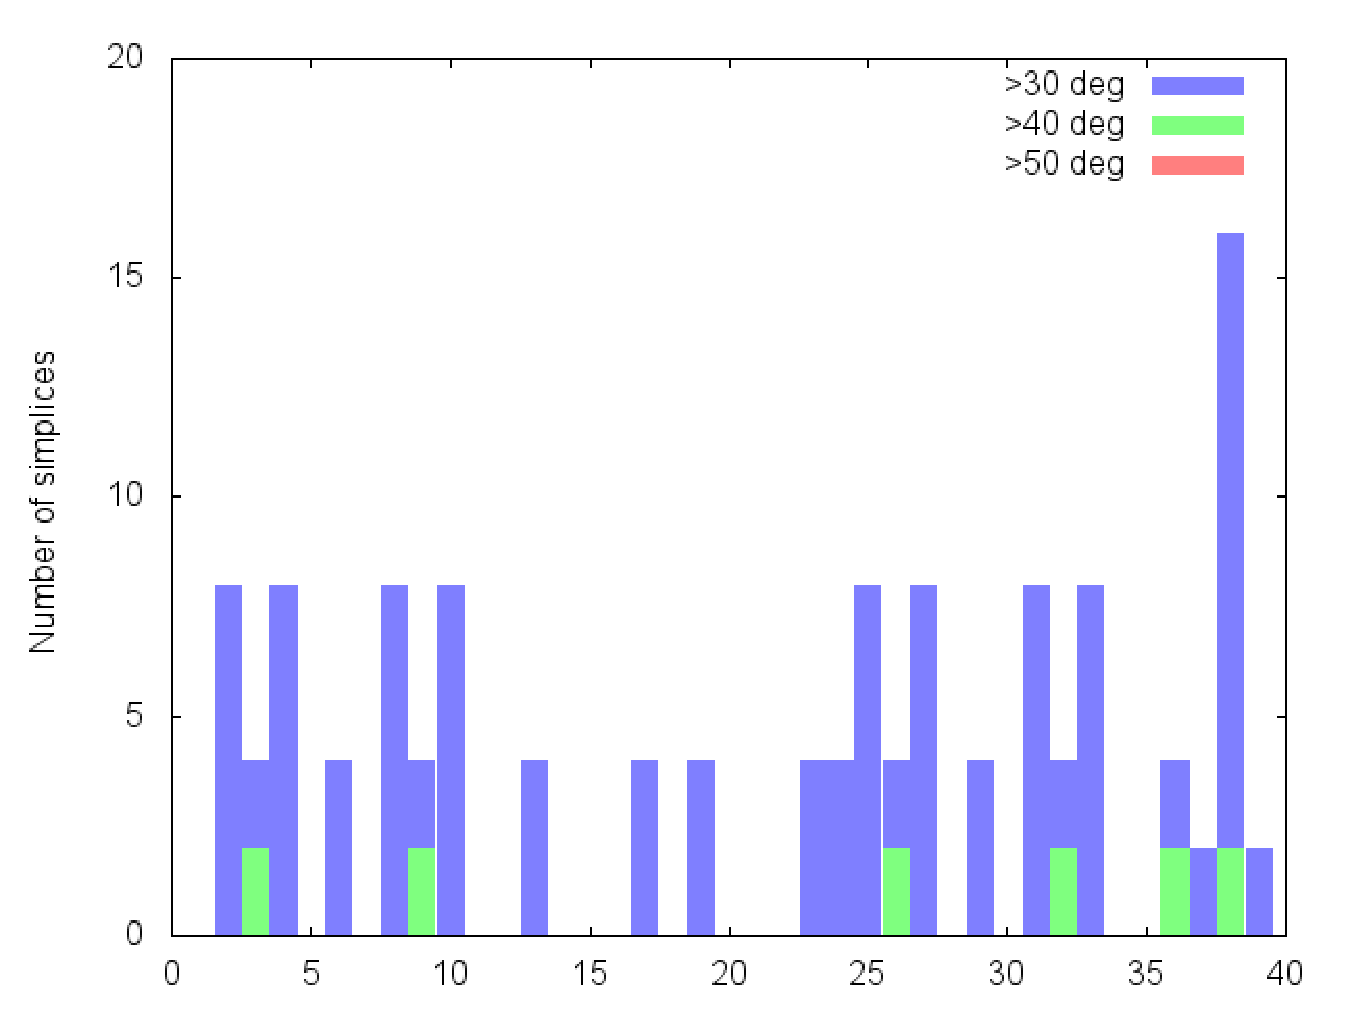
\includegraphics[width=0.3\linewidth]{images/ms_euro_flange_distribution.eps}\label{fig:msharp:flange:c}} &
	\subfloat[TwoCubes: Triangle normal differences]{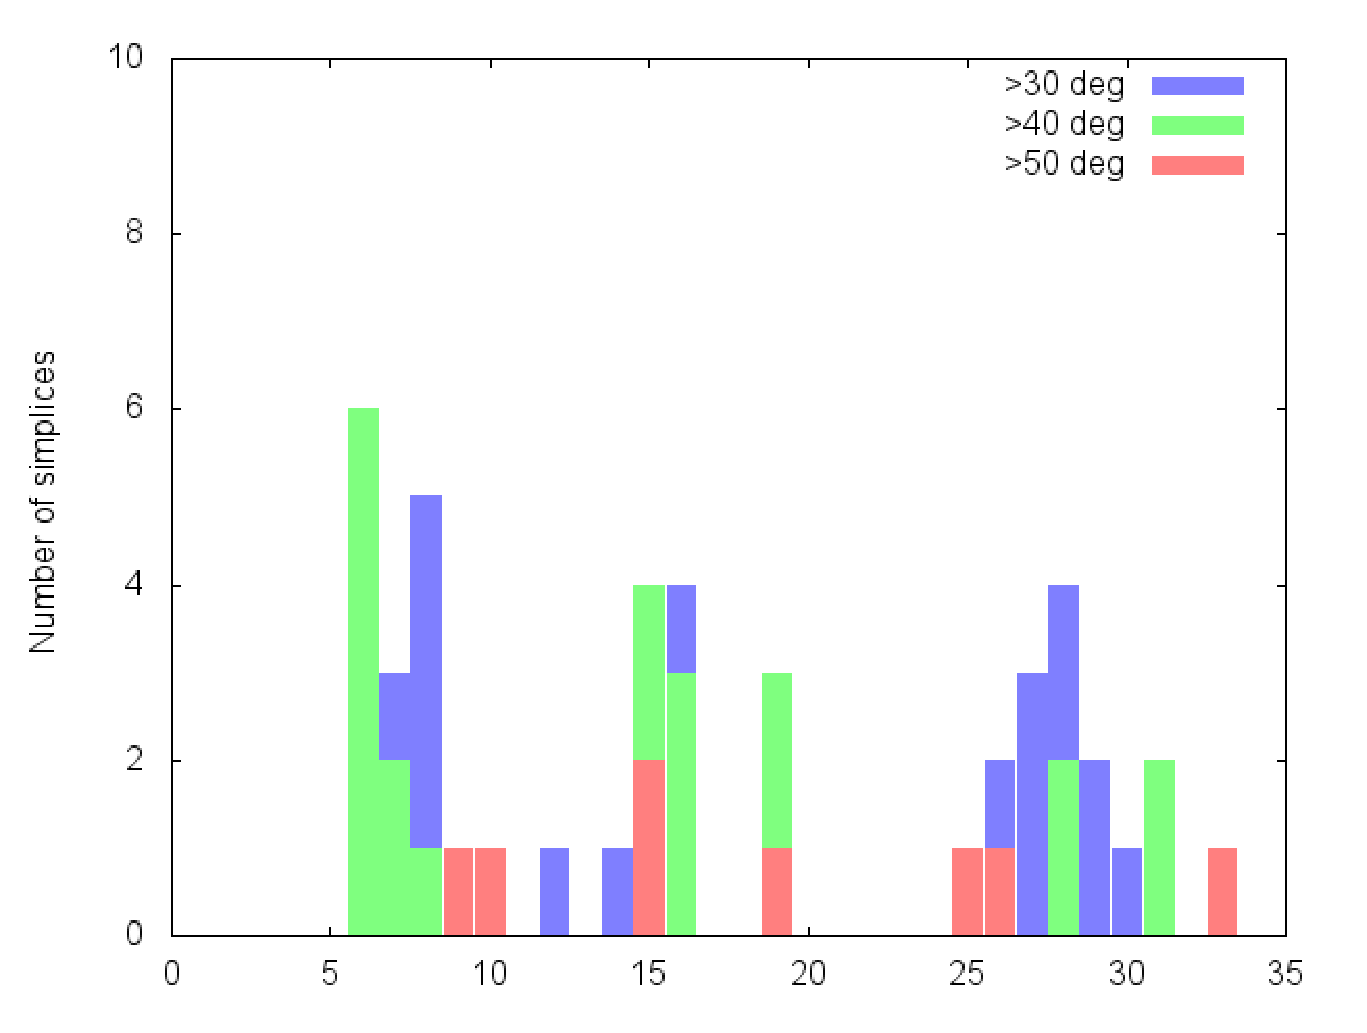
\includegraphics[width=0.3\linewidth]{images/ms_euro_twoCube_distribution.eps}\label{fig:msharp:tc:c}} \\
	\subfloat[Notch in MergeSharp Flange isosurface]{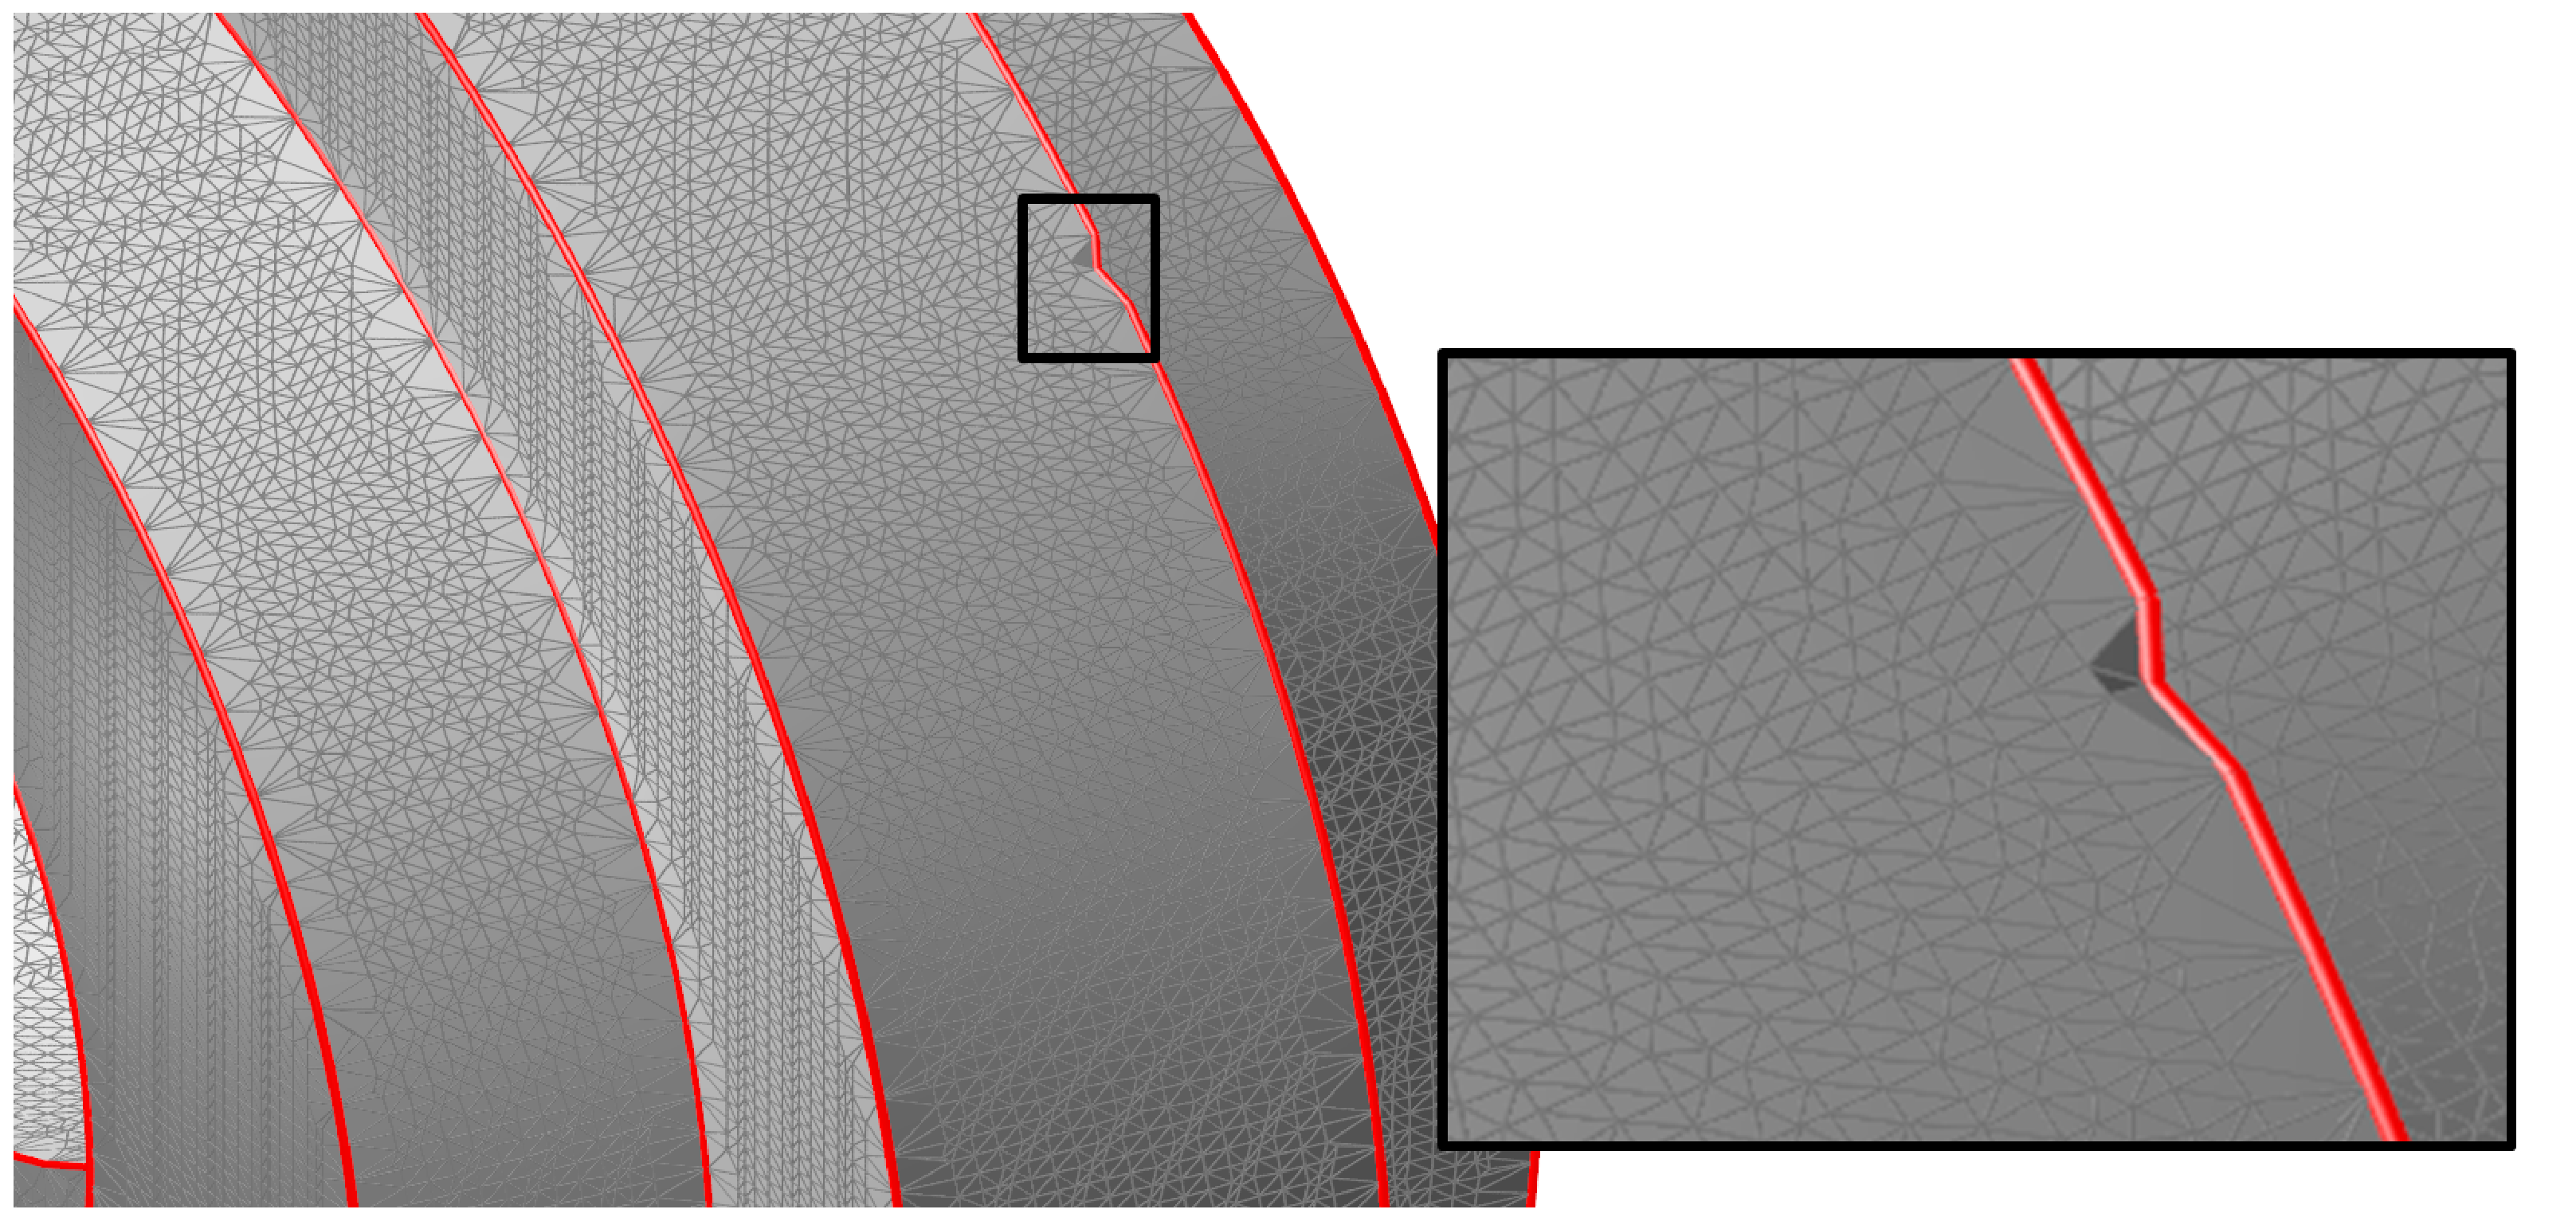
\includegraphics[width=0.3\linewidth]{images/mergeSharpvsShrec2.eps}\label{fig:msharp:b}} &
	\subfloat[Dimpled MergeSharp isosurface (left) and smooth SHREC isosurface (right)]{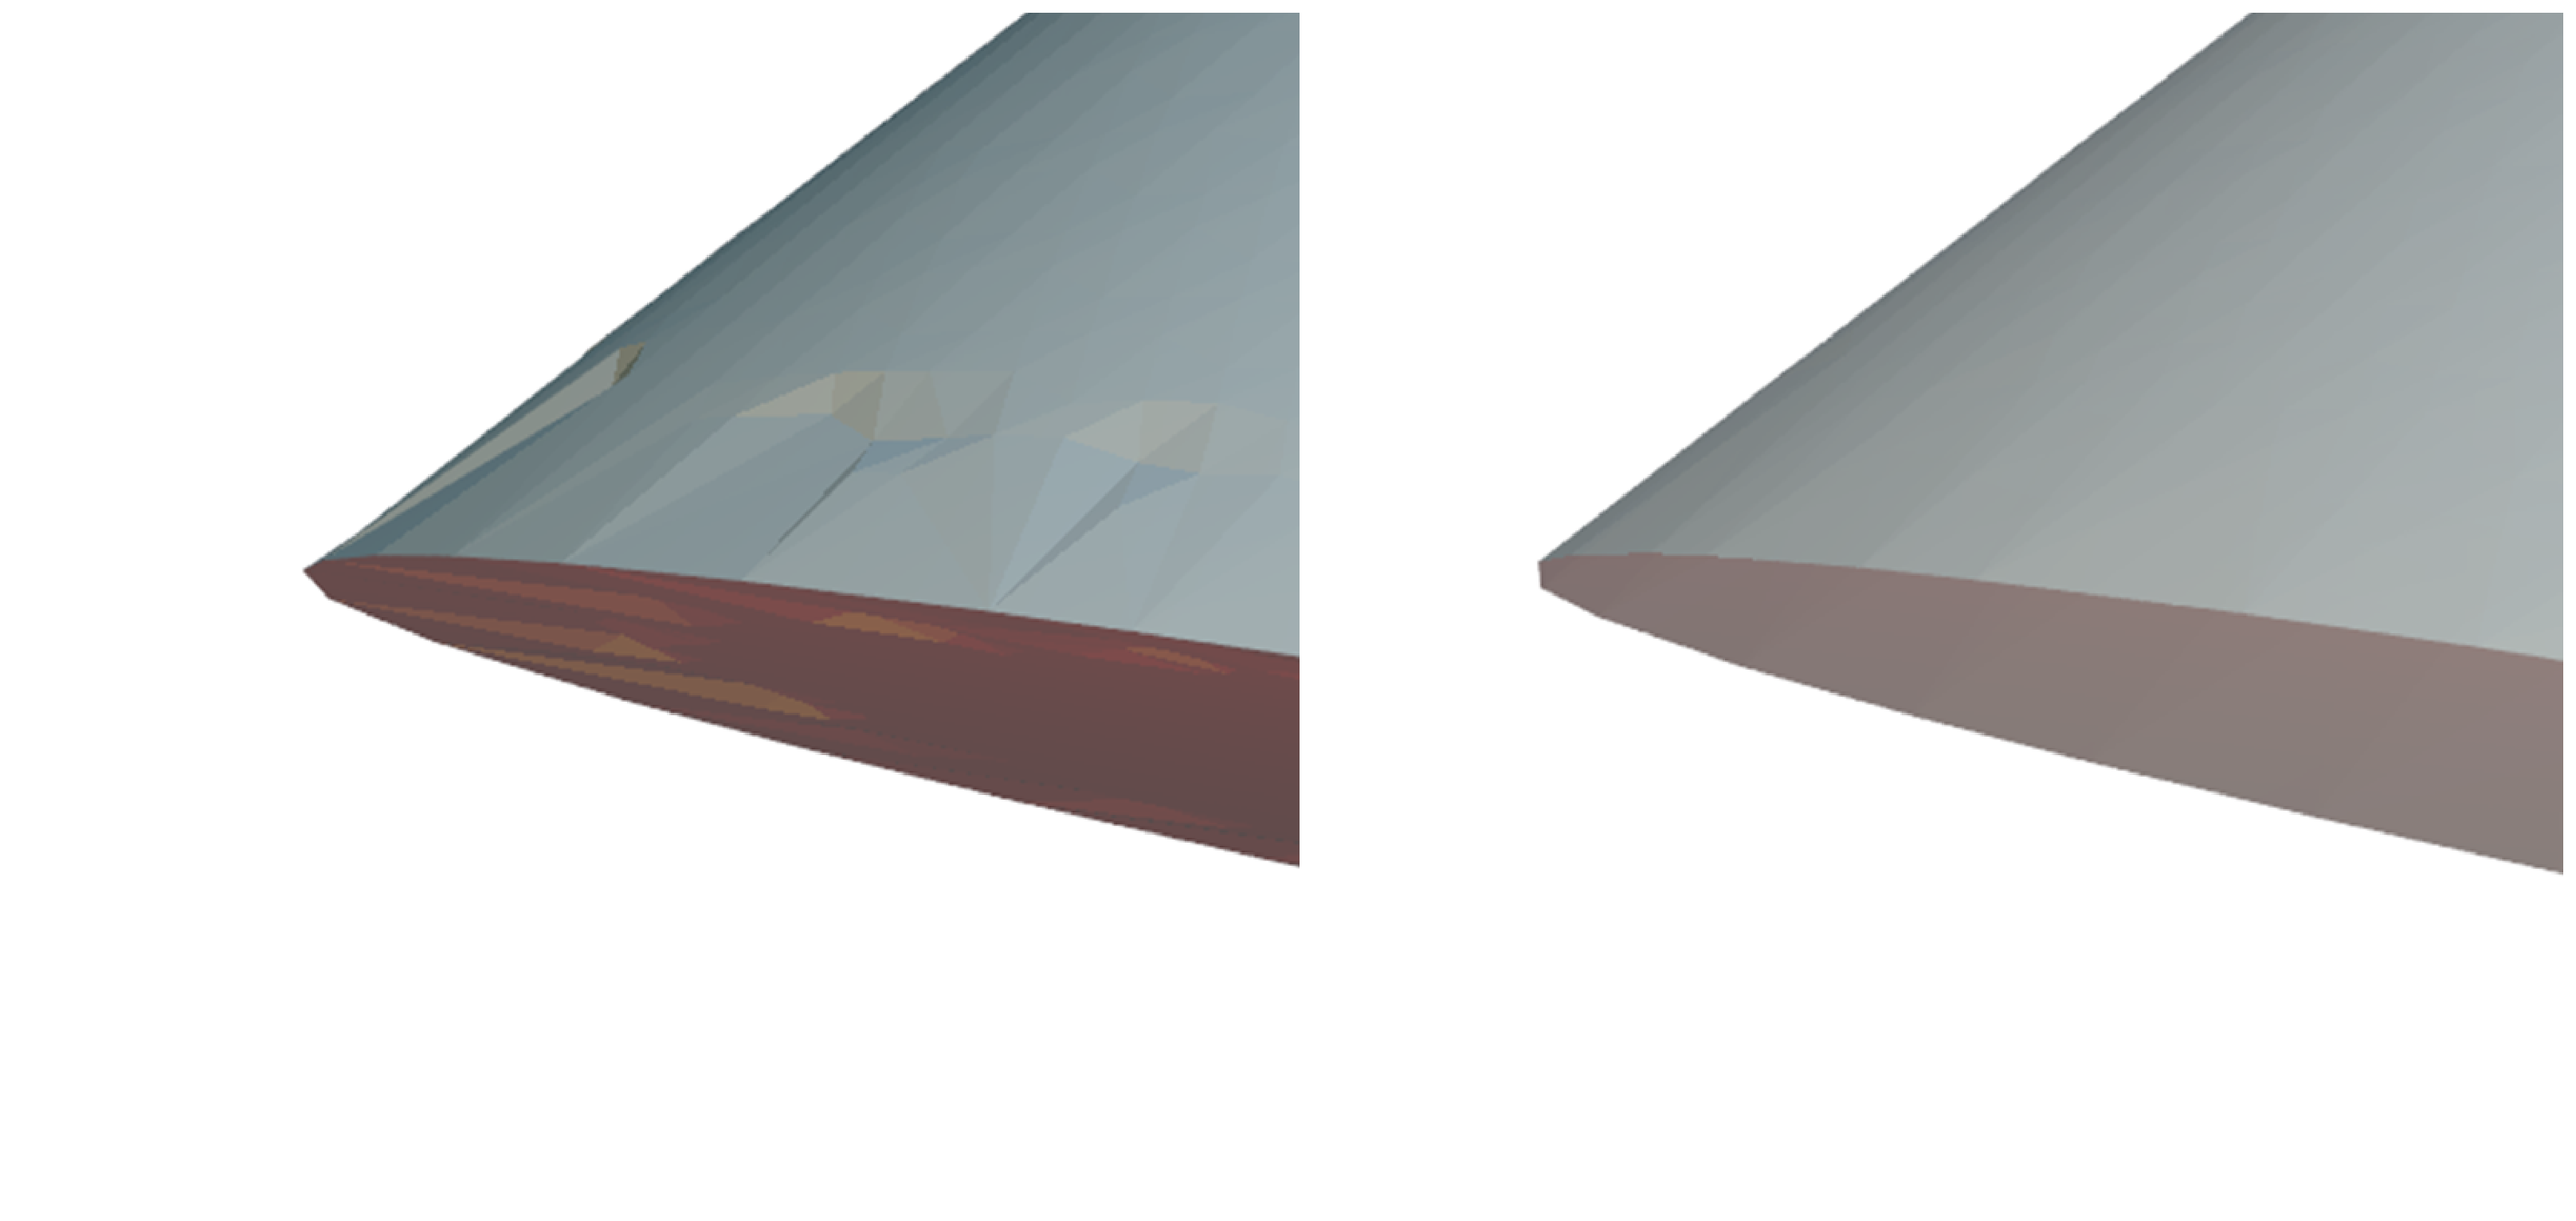
\includegraphics[width=0.3\linewidth]{images/cone_mergesharp.eps}\label{fig:msharp:c}}
\end{tabular}
	\caption{Results of  MergeSharp on 40 Flange and 34 TwoCubes data sets
(exact gradients).
	\protect\subref{fig:msharp:flange:A}~Angle distance to polygonal Flange meshes.
	\protect\subref{fig:msharp:flange:D}~Degree errors in 1-skeleton 
of sharp edges of Flange datasets.
	\protect\subref{fig:msharp:tc:A}~Angle distance to polygonal TwoCubes meshes.
	\protect\subref{fig:msharp:tc:D}~Degree errors in 1-skeleton 
of sharp edges of TwoCubes datasets.
	\protect\subref{fig:msharp:tc:c}~Number of triangles 
with angle difference to polygonal Flange mesh above 30, 40 and 50 degrees.
(No Flange isosurface triangles have angle difference above $50^\circ$.)
	\protect\subref{fig:msharp:flange:c}~Number of triangles 
with angle difference to polygonal TwoCubes mesh above 30, 40 and 50 degrees.
	 \protect\subref{fig:msharp:b}~Notch in a MergeSharp Flange isosurface.
	 \protect\subref{fig:msharp:c}~Dimples 
in a MergeSharp Cone isosurface (left).
Compare with smooth SHREC isosurface (right).}
\label{fig:msharp}
\end{figure*}	

\section{Comparison with Other Algorithms}
\label{section:comparison}

We compared SHREC with software implementations of four other algorithms:
MergeSharp~\cite{bw-cisec-13,bw-erm-13}, 
PolyMender~\cite{j-rrpm-04}, 
EMC (Extended Marching Cubes)~\cite{kbsh-fssev-01} 
and SingularCocone~\cite{Dey2012}.
Table~\ref{table:software} contains descriptions of the software.

Input to both SHREC and MergeSharp is a regular grid sampling
of a scalar field and the gradients at the grid vertices.
Input to the software implementations of the other algorithms
is very different from input to SHREC or inputs to each other,
so one should be extremely careful in make comparisons
between these algorithms based on the results presented here.
For instance, on average,
EMC has fewer degree errors
than PolyMender or SingularCocone,
but EMC computes scalar, 
distance and normal values from formulas hard wired into the software.
PolyMender and SingularCocone (and SHREC and MergeSharp)
would certainly do much better if their input came
from formulas hard wired into their software.

SingularCocone has the most degree errors,
but SingularCocone is designed for reconstruction 
from point samples of a (possibly non-manifold) surface,
not for reconstruction from sampling of a scalar field.
Input to SingularCocone is point samples of a surface,
not scalar grid or gradient information.


\begin{figure*}[t]
	\centering
			\subfloat[]{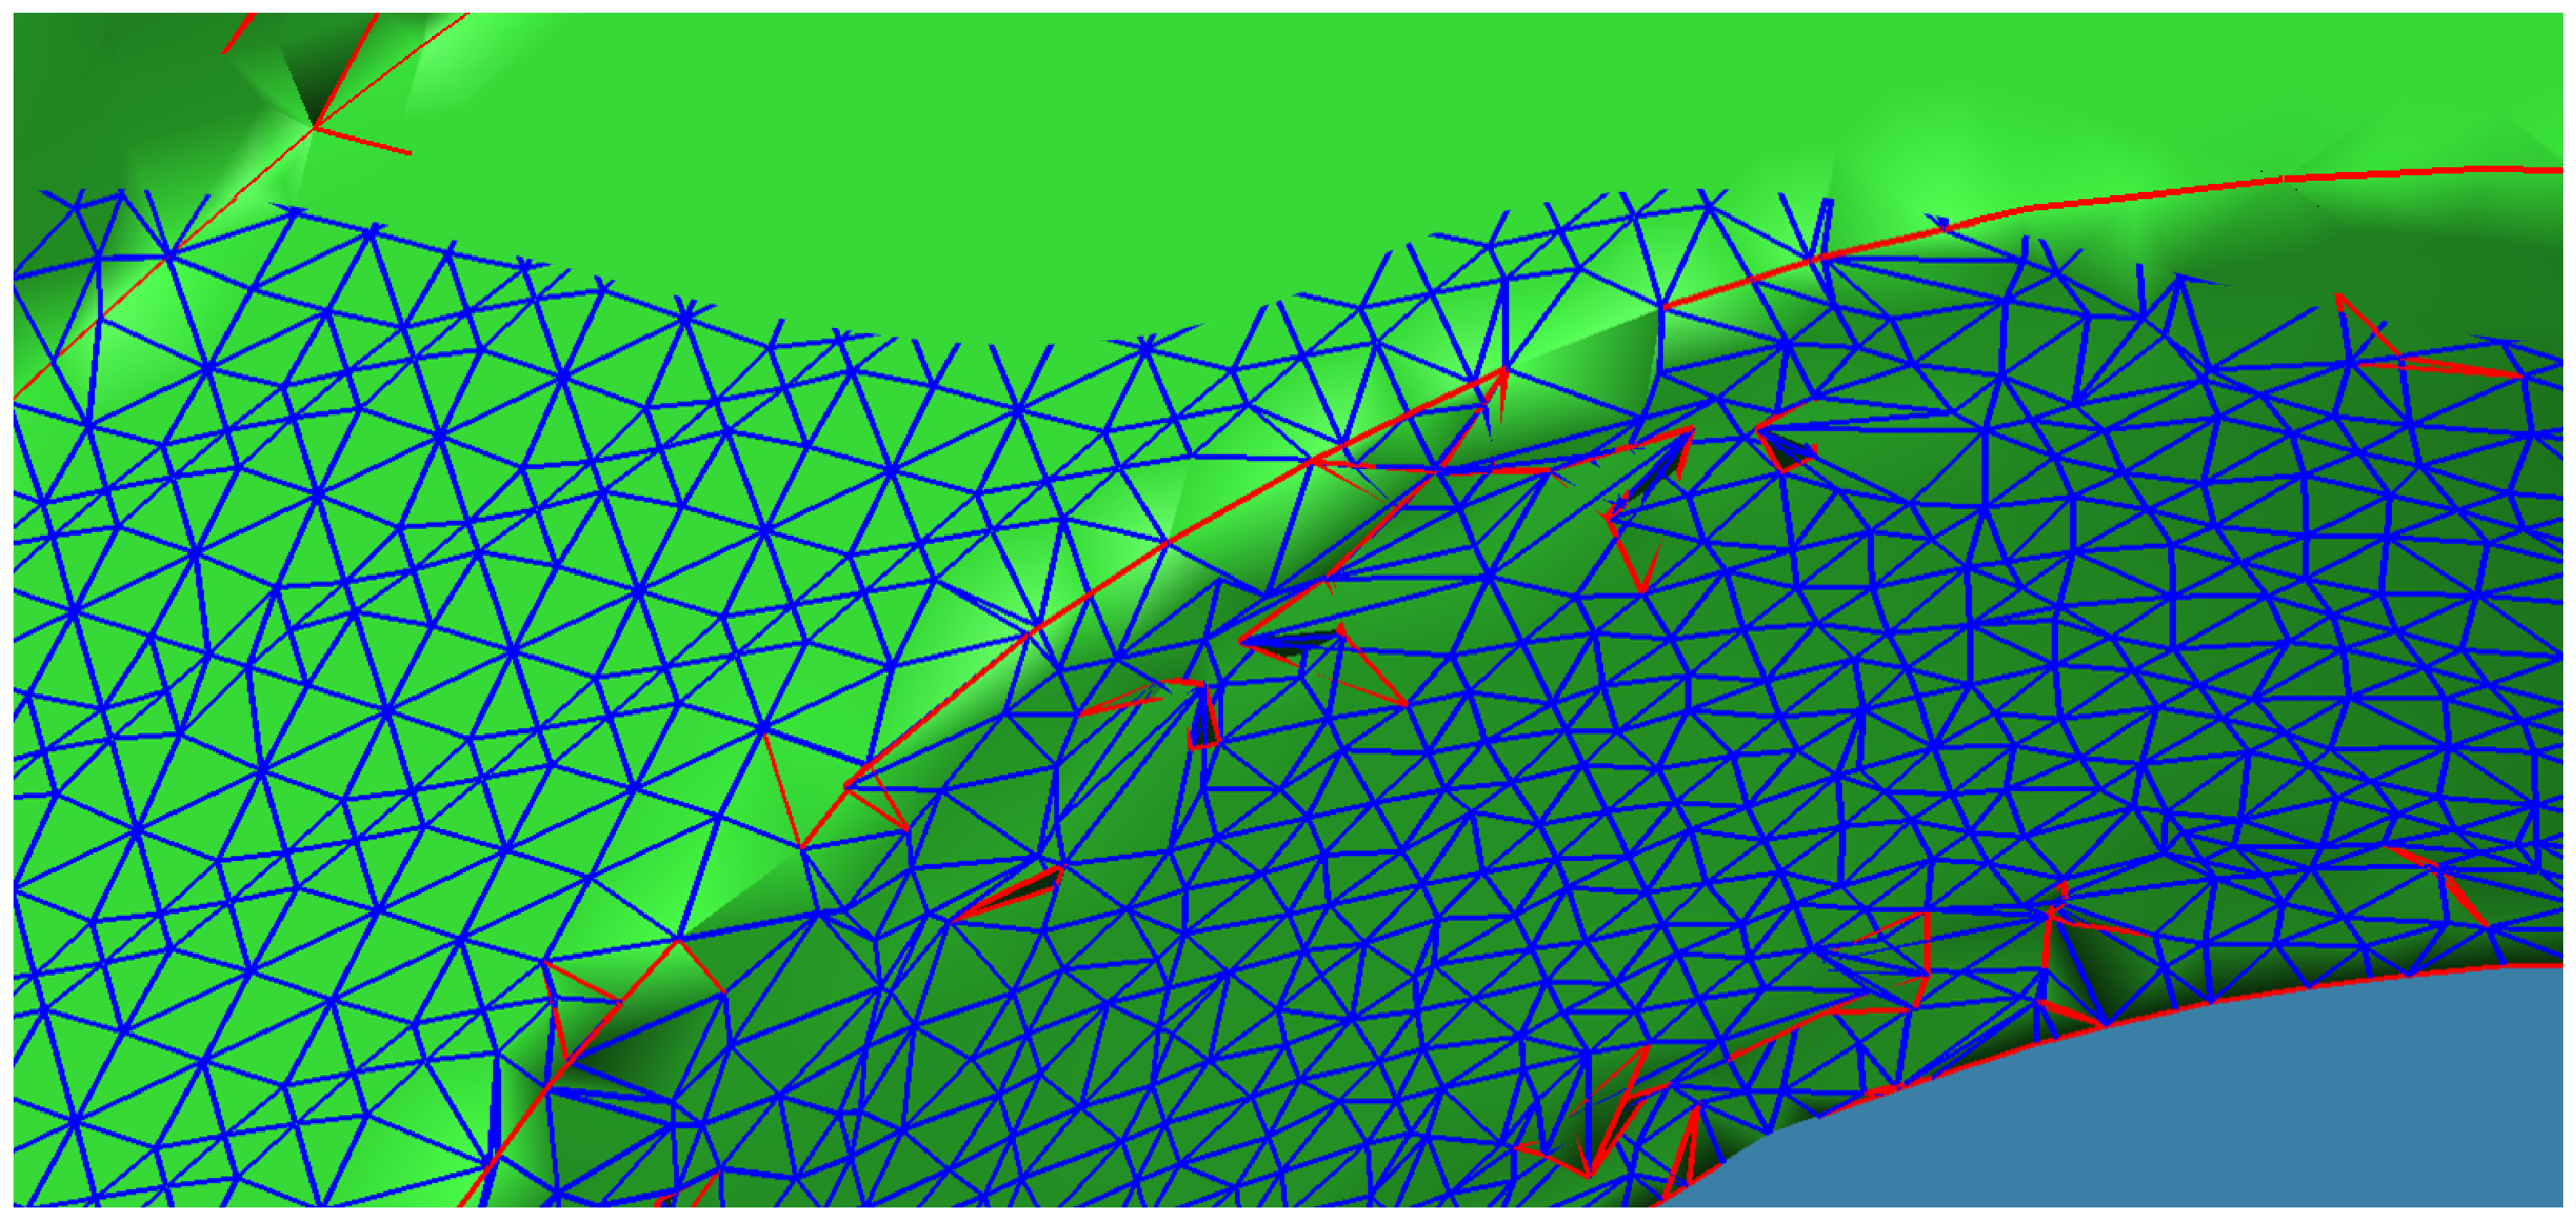
\includegraphics[width=0.33\linewidth]{images/polymender4.eps}\label{fig:polymenderB:b}}\quad
			\subfloat[]{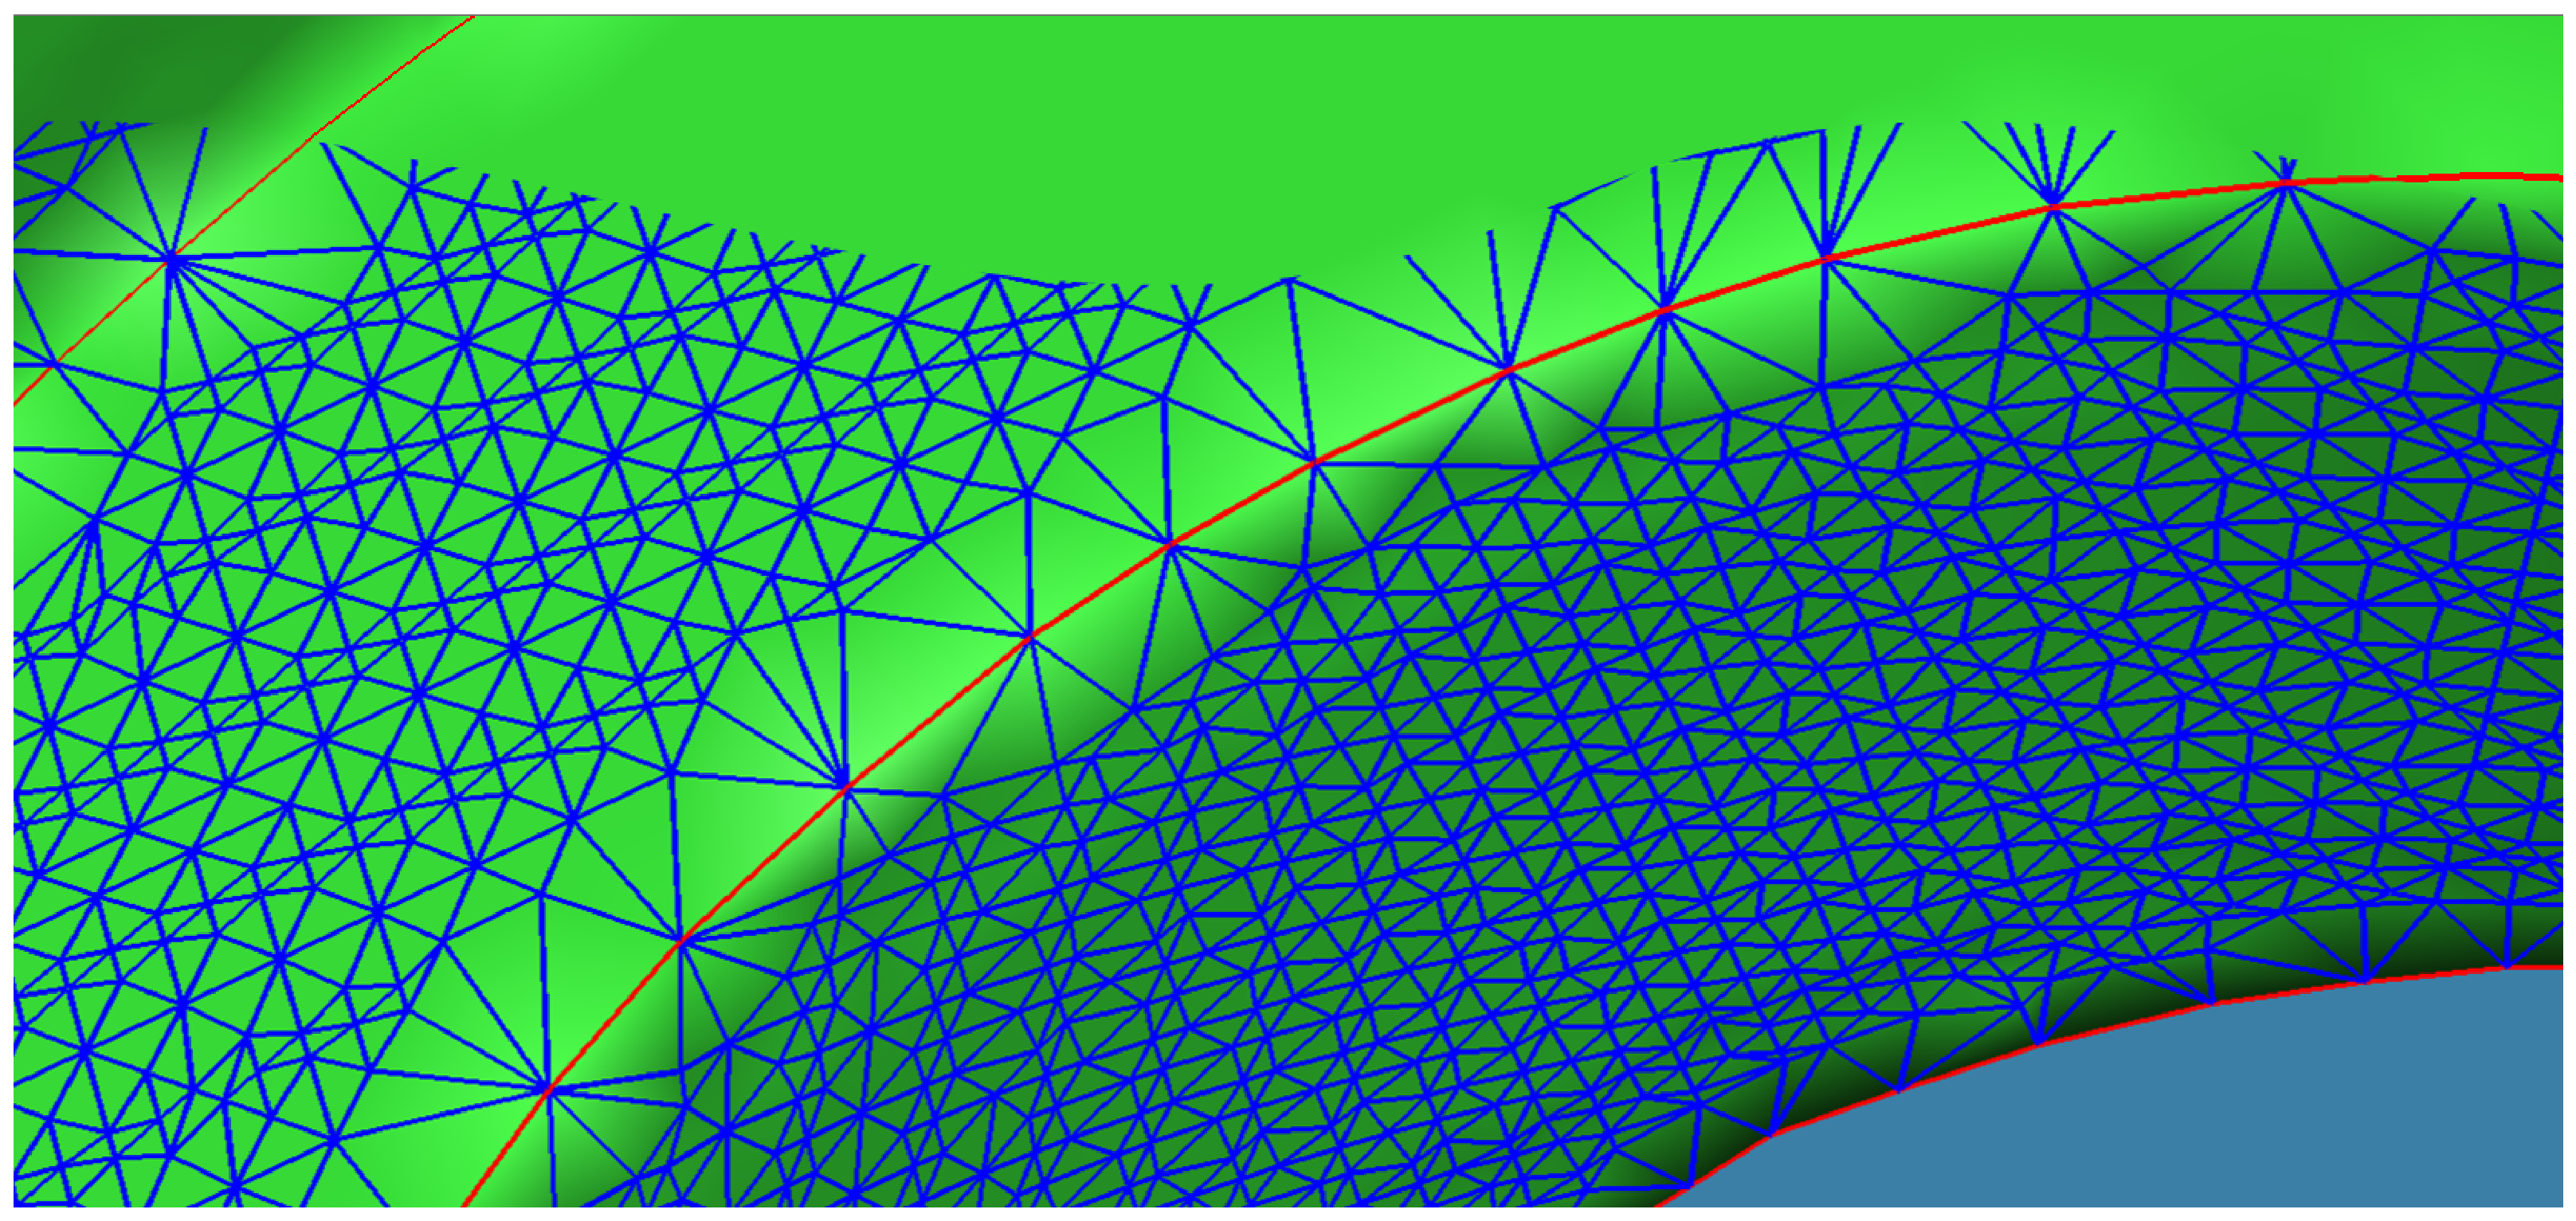
\includegraphics[width=0.33\linewidth]{images/polymender3.eps}\label{fig:polymenderB:a}}
			\subfloat[]{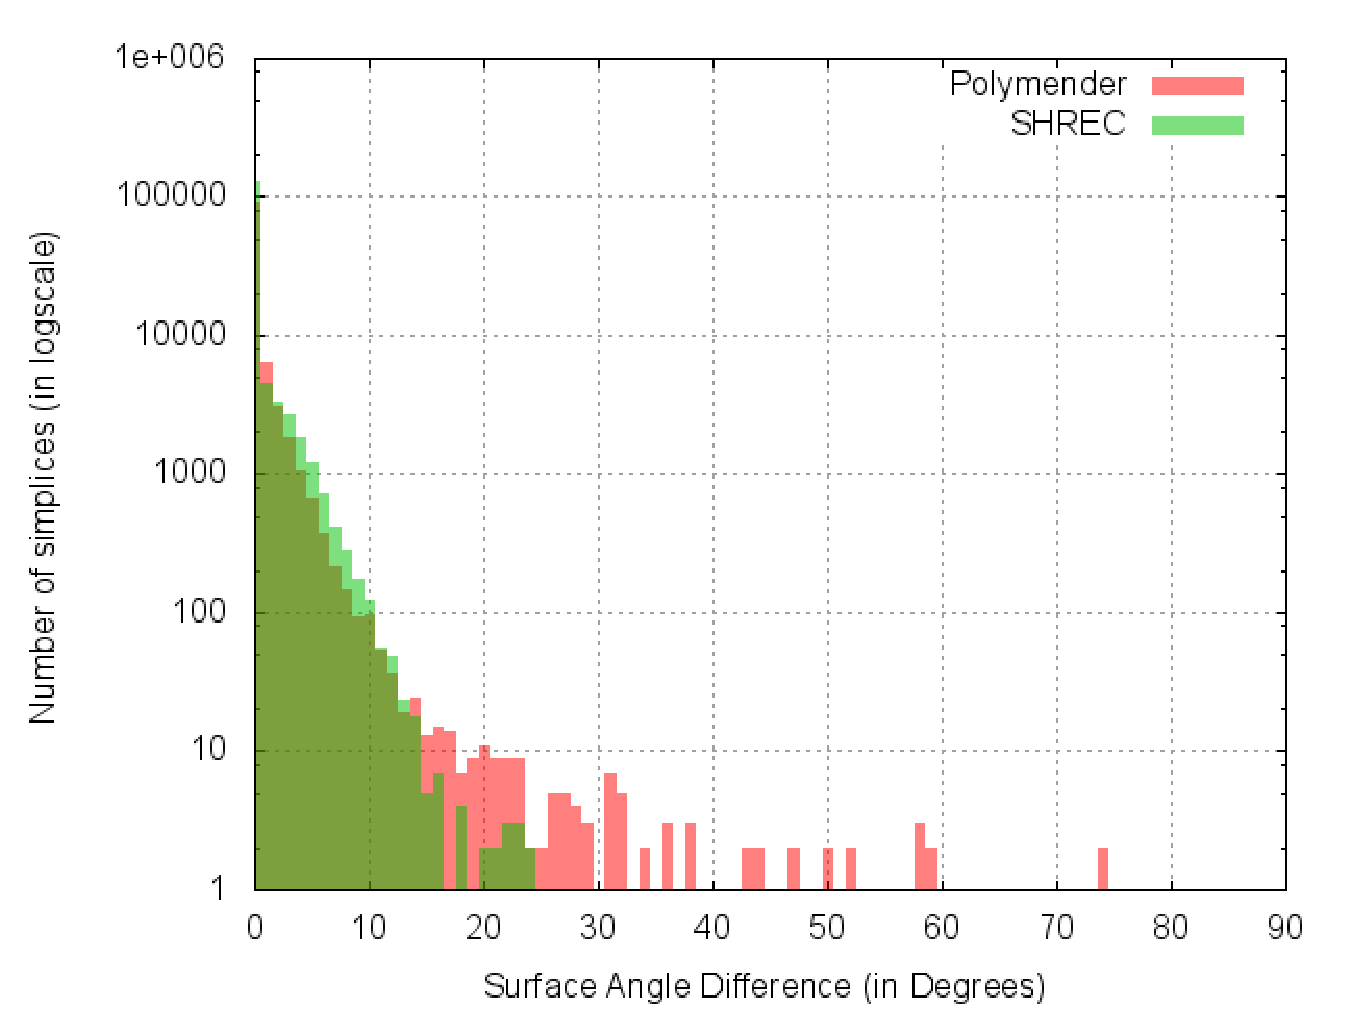
\includegraphics[width=0.3\linewidth]{images/polymenderHistogram_1.eps}\label{fig:polymenderB:c}}\\
			\subfloat[]{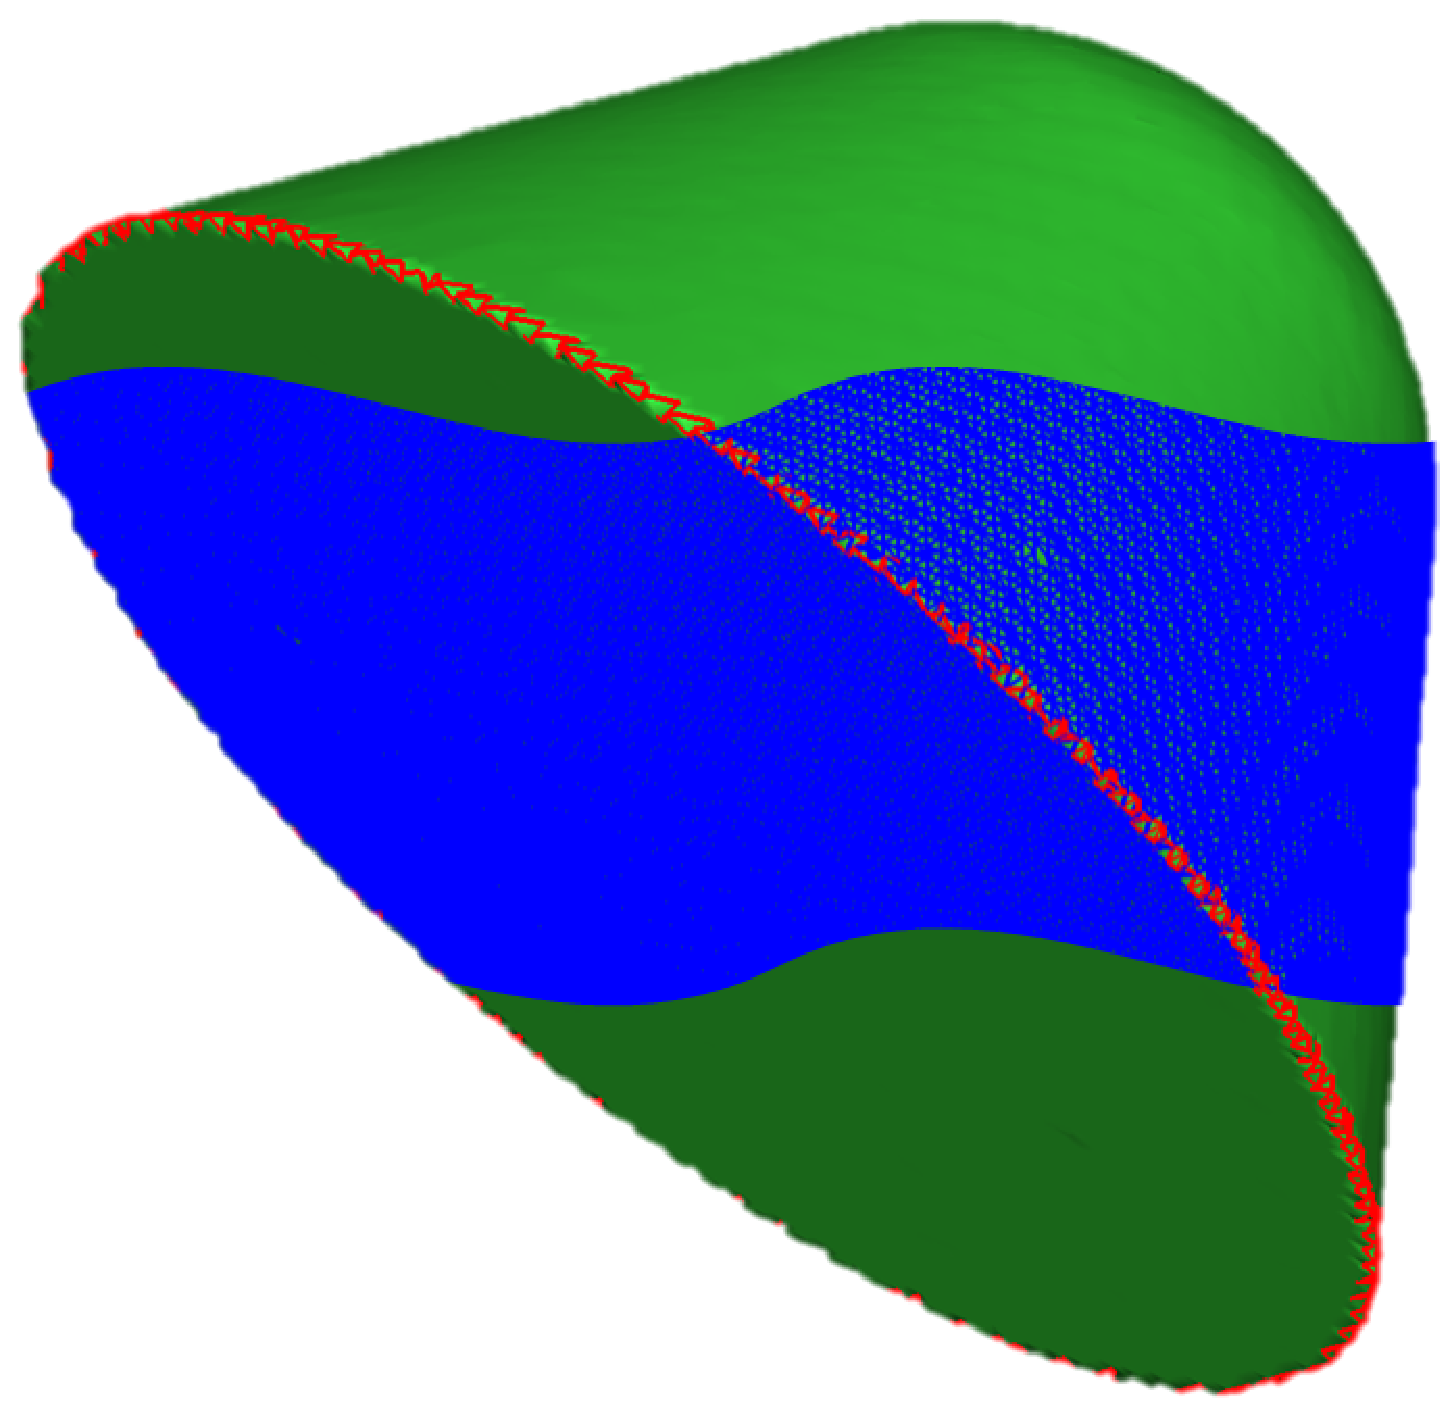
\includegraphics[width=0.2\linewidth]{images/polymender_cone_merge_2.eps}\label{fig:polymender:cone:b}}\quad
			\subfloat[]{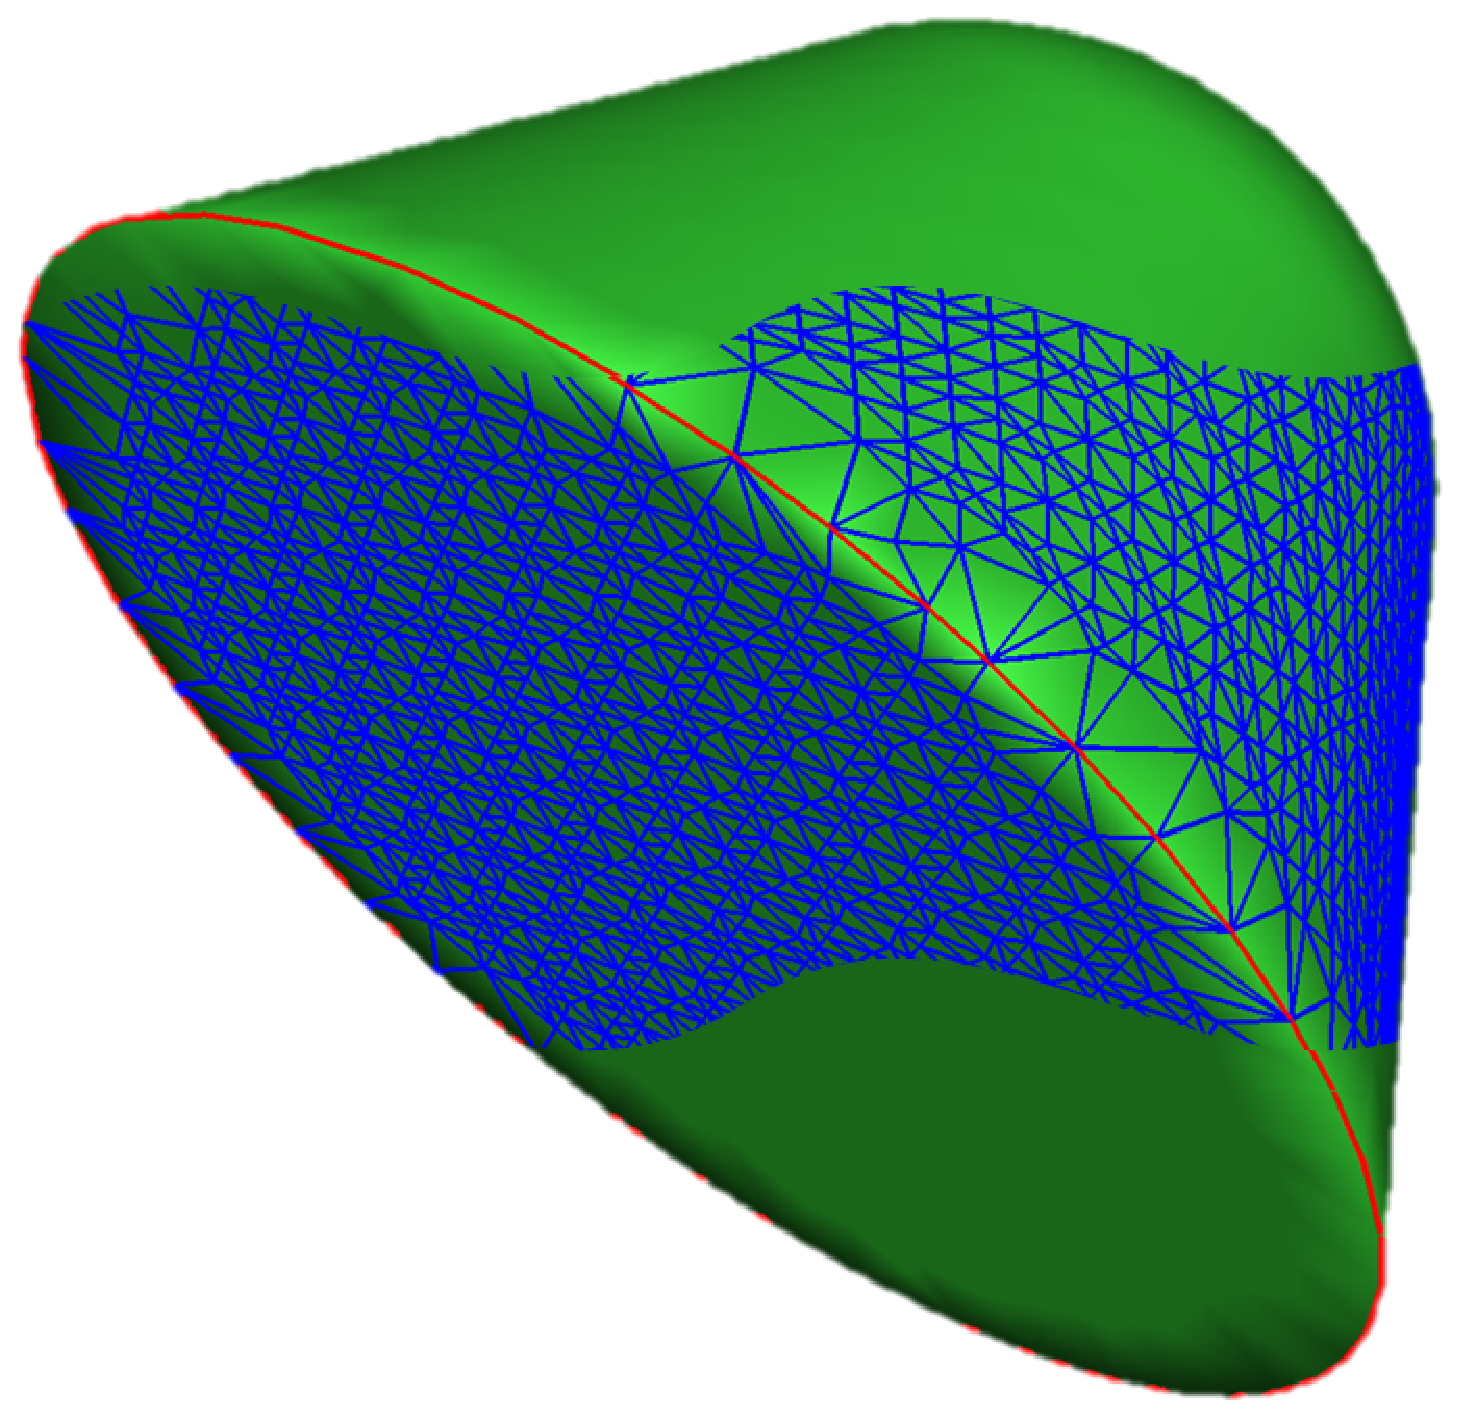
\includegraphics[width=0.2\linewidth]{images/polymender_cone_merge_1.eps}\label{fig:polymender:cone:a}}\quad
			\subfloat[]{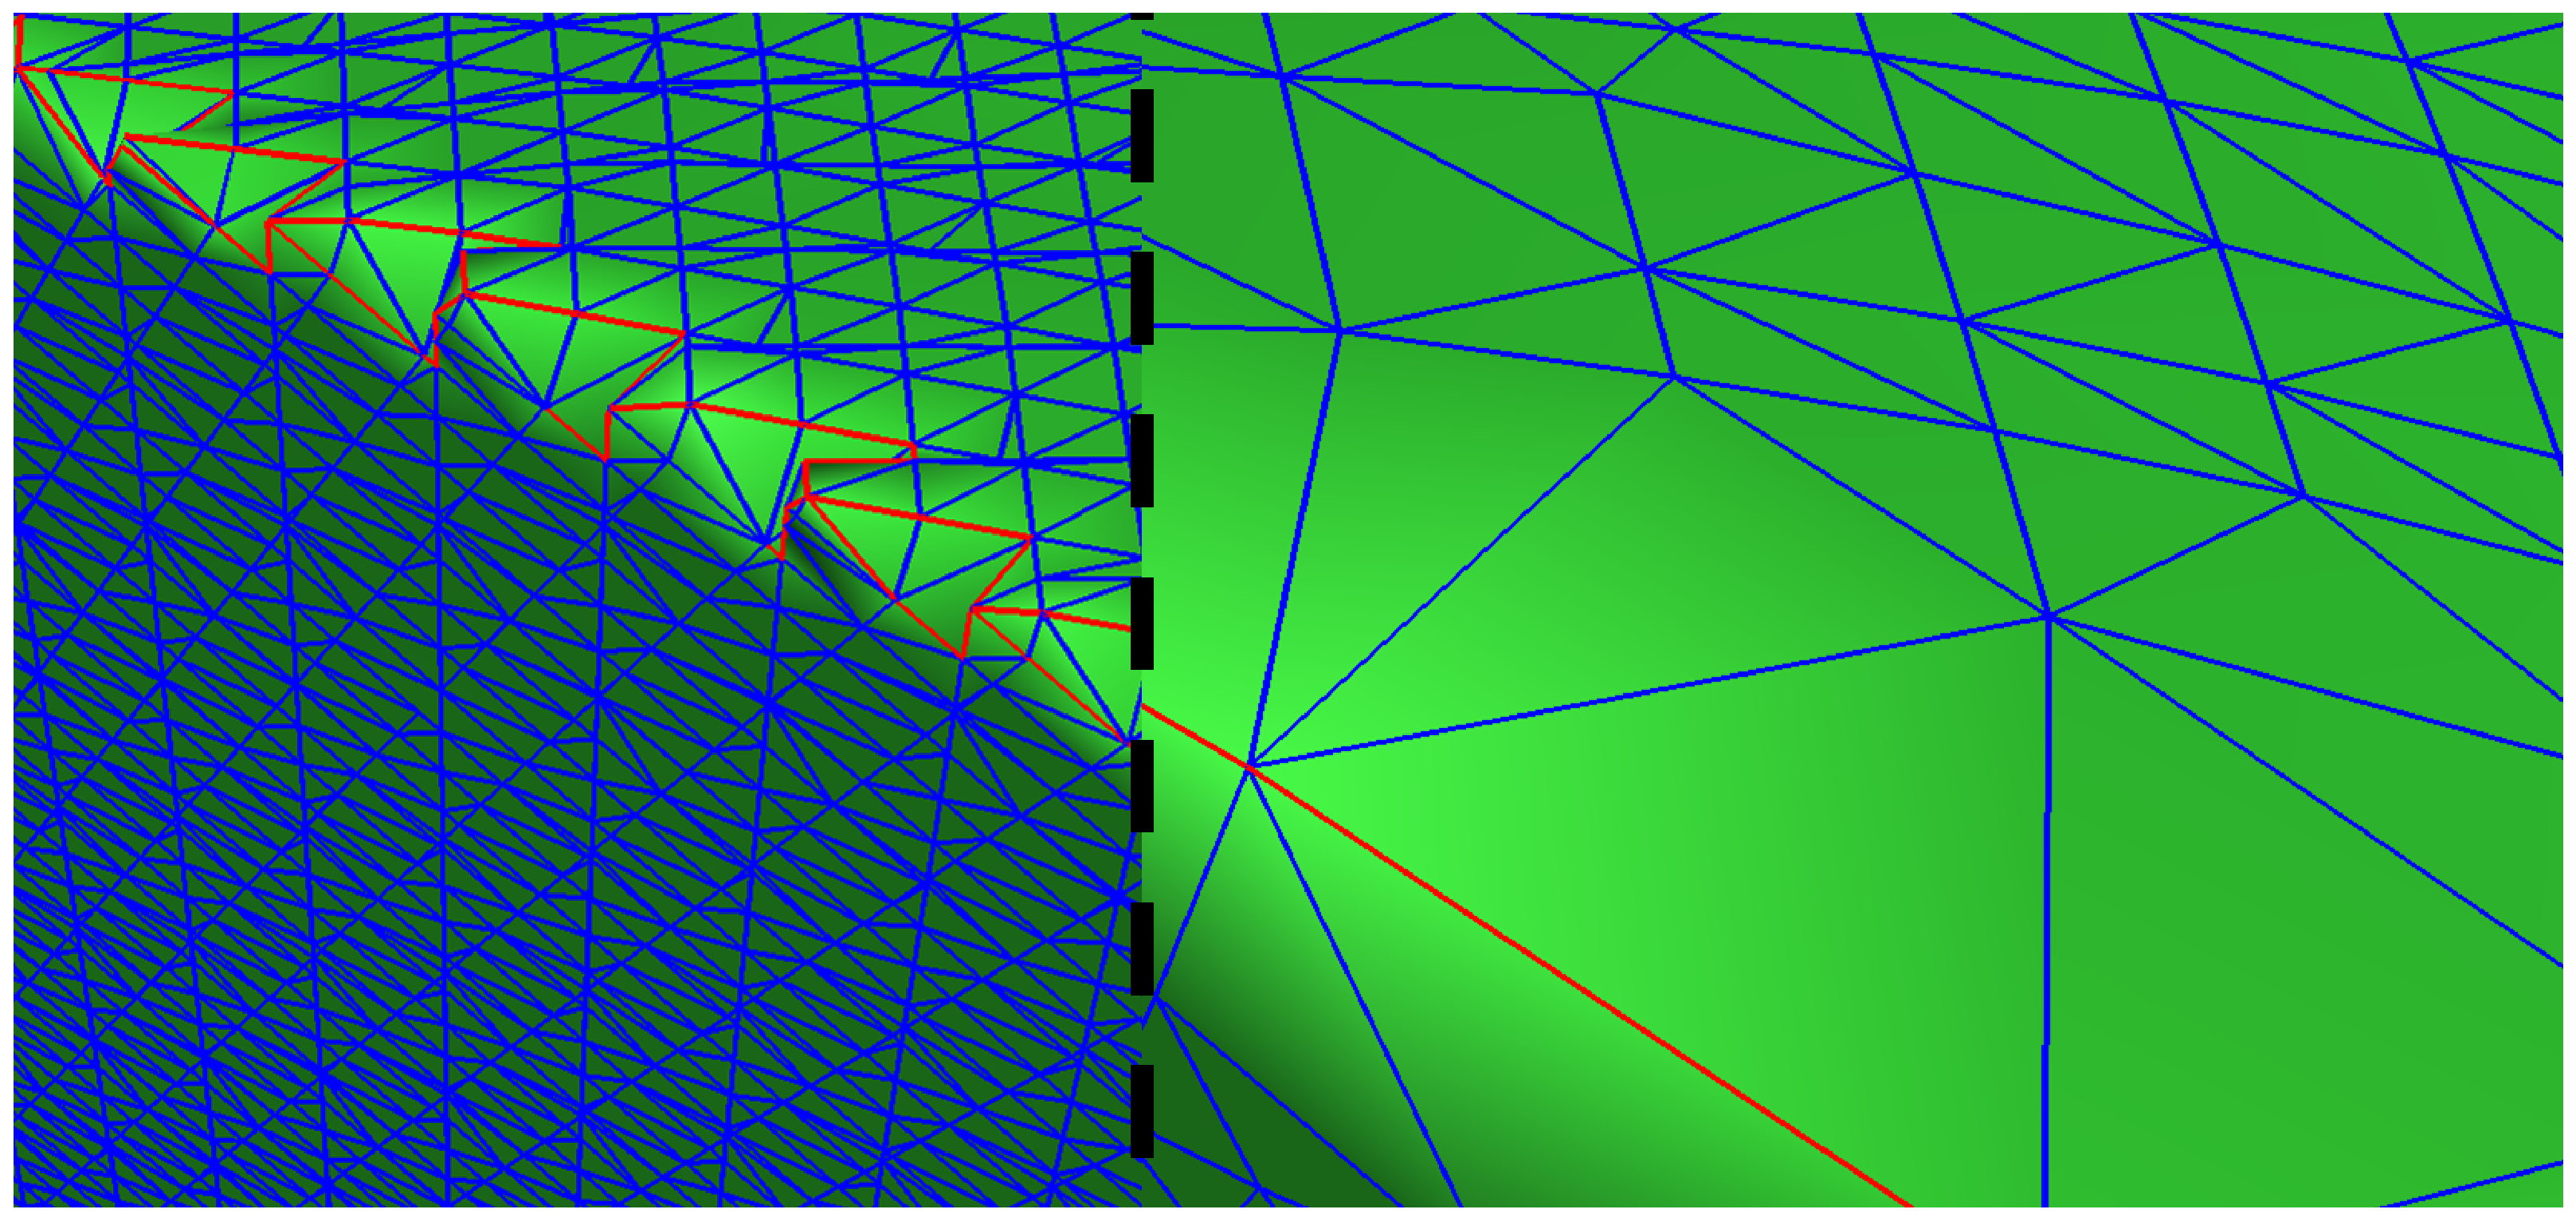
\includegraphics[width=0.4\linewidth]{images/polymender_cone_merge_3.eps}\label{fig:polymender:cone:c}}

\caption{PolyMender and SHREC comparison.
Mesh edges with dihedral angle below $140^\circ$ are colored red.
\protect\subref{fig:polymenderB:b}~PolyMender Flange isosurface.
\protect\subref{fig:polymenderB:a}~Corresponding SHREC Flange isosurface.
\protect\subref{fig:polymenderB:c} Distribution of differences of triangle normals
between PolyMender isosurface and polyhedral mesh (red)
and between SHREC isosurface and polyhedral mesh (green).
\protect\subref{fig:polymender:cone:b} PolyMender Cone isosurface.
\protect\subref{fig:polymender:cone:a} Corresponding SHREC Cone isosurface.
\protect\subref{fig:polymender:cone:c} Magnified view of Polymender isosurface (left)
and corresponding SHREC isosurface (right).
} 
\label{fig:polymenderB}
\end{figure*}


\paragraph{Comparison with MergeSharp.}

%mergesharp_euro =['E:\\Programs\\Win\\stdAlone\\ijk\\bin\\mergesharpbin\\Release\\mergesharp.exe', '-position', 'gradNS', '-trimesh']
%def compare_with_euro(n, iso):

Input to MergeSharp is a regular grid sampling of a scalar field
and the gradients at the grid vertices.
We ran MergeSharp on the same 40 Flange and 34 TwoCube synthetic datasets
that we applied to SHREC in Section~\ref{section:synthetic_tests}.
We used the exact gradients on MergeSharp, not the Religrad gradients.
Figures~\subref*{fig:msharp:flange:A} and~\subref*{fig:msharp:tc:c}
shows the oriented angle distance between the MergeSharp isosurfaces 
and the polyhedral mesh isosurfaces.
Five of the MergeSharp TwoCubes isosurfaces have angle distance 
near $180^\circ$ indicating ``flipped'' triangles produced by folds
in the mesh.
Figures~\ref{fig:msharp:flange:c} and~\ref{fig:msharp:tc:c} 
present the number of triangles with angle difference greater
than $30$, $40$ and $50$ degrees 
in the MergeSharp Flange and TwoCubes isosurfaces.
24 out of 40 of the Flange isosurfaces and 18 out of 34 
of the TwoCube isosurface have angle distance above $30^\circ$
indicating significant problems in the reconstruction of sharp features.

Figures~\subref*{fig:msharp:flange:D} and~\subref*{fig:msharp:tc:D}
gives the number of degree errors in the 1-skeleton's of the sharp edges.
8 out of 40 of the Flange isosurfaces and 15 out of 34 of the TwoCube
isosurfaces have degree errors.
The maximum number of degree errors is eight.

Note that all the results in Figure~\ref{fig:msharp} are
for MergeSharp isosurfaces produced from EXACT gradients.
Thus, they should not be compared with the SHREC results
in Figure~\ref{fig:flangeAngle} for Flange isosurfaces
produced using Religrad gradients.
The 40 SHREC Flange isosurfaces produced using exact gradients
all have angle distance under ???
compared with angle distances above $30^\circ$
for 24 of the corresponding MergeSharp isosurfaces.
None of the SHREC Flange isosurfaces produced using exact gradients
have degree errors
compared with 8 MergeSharp isosurfaces with 4 to 8 degree errors.

As shown in Figure~\ref{fig:shrecTwoCube}(a),
the 40 SHREC TwoCube isosurfaces produced using exact gradients
all have angle distance under $2^\circ$.
(Note the y-scale in Figure~\ref{fig:shrecTwoCube}(a)
is from 0 to $10^\circ$.)
18 of the corresponding MergeSharp TwoCube isosurfaces have
angle distance above $30^\circ$.
None of the SHREC TwoCubes isosurfaces produced using exact gradients
have degree errors
compared with 15 of the TwoCube isosurfaces with 2 to 5 degree errors.

Figure~\protect\subref*{fig:msharp:b} shows ``notches''
in a MergeSharp Flange isosurface.
Figure~\protect\subref*{fig:msharp:c} shows gentle dimples
in a MergeSharp Cone isosurface (left image).
The corresponding SHREC isosurface is smooth and does not have these dimples.

\begin{figure*}[p]
	\centering
		\subfloat[]{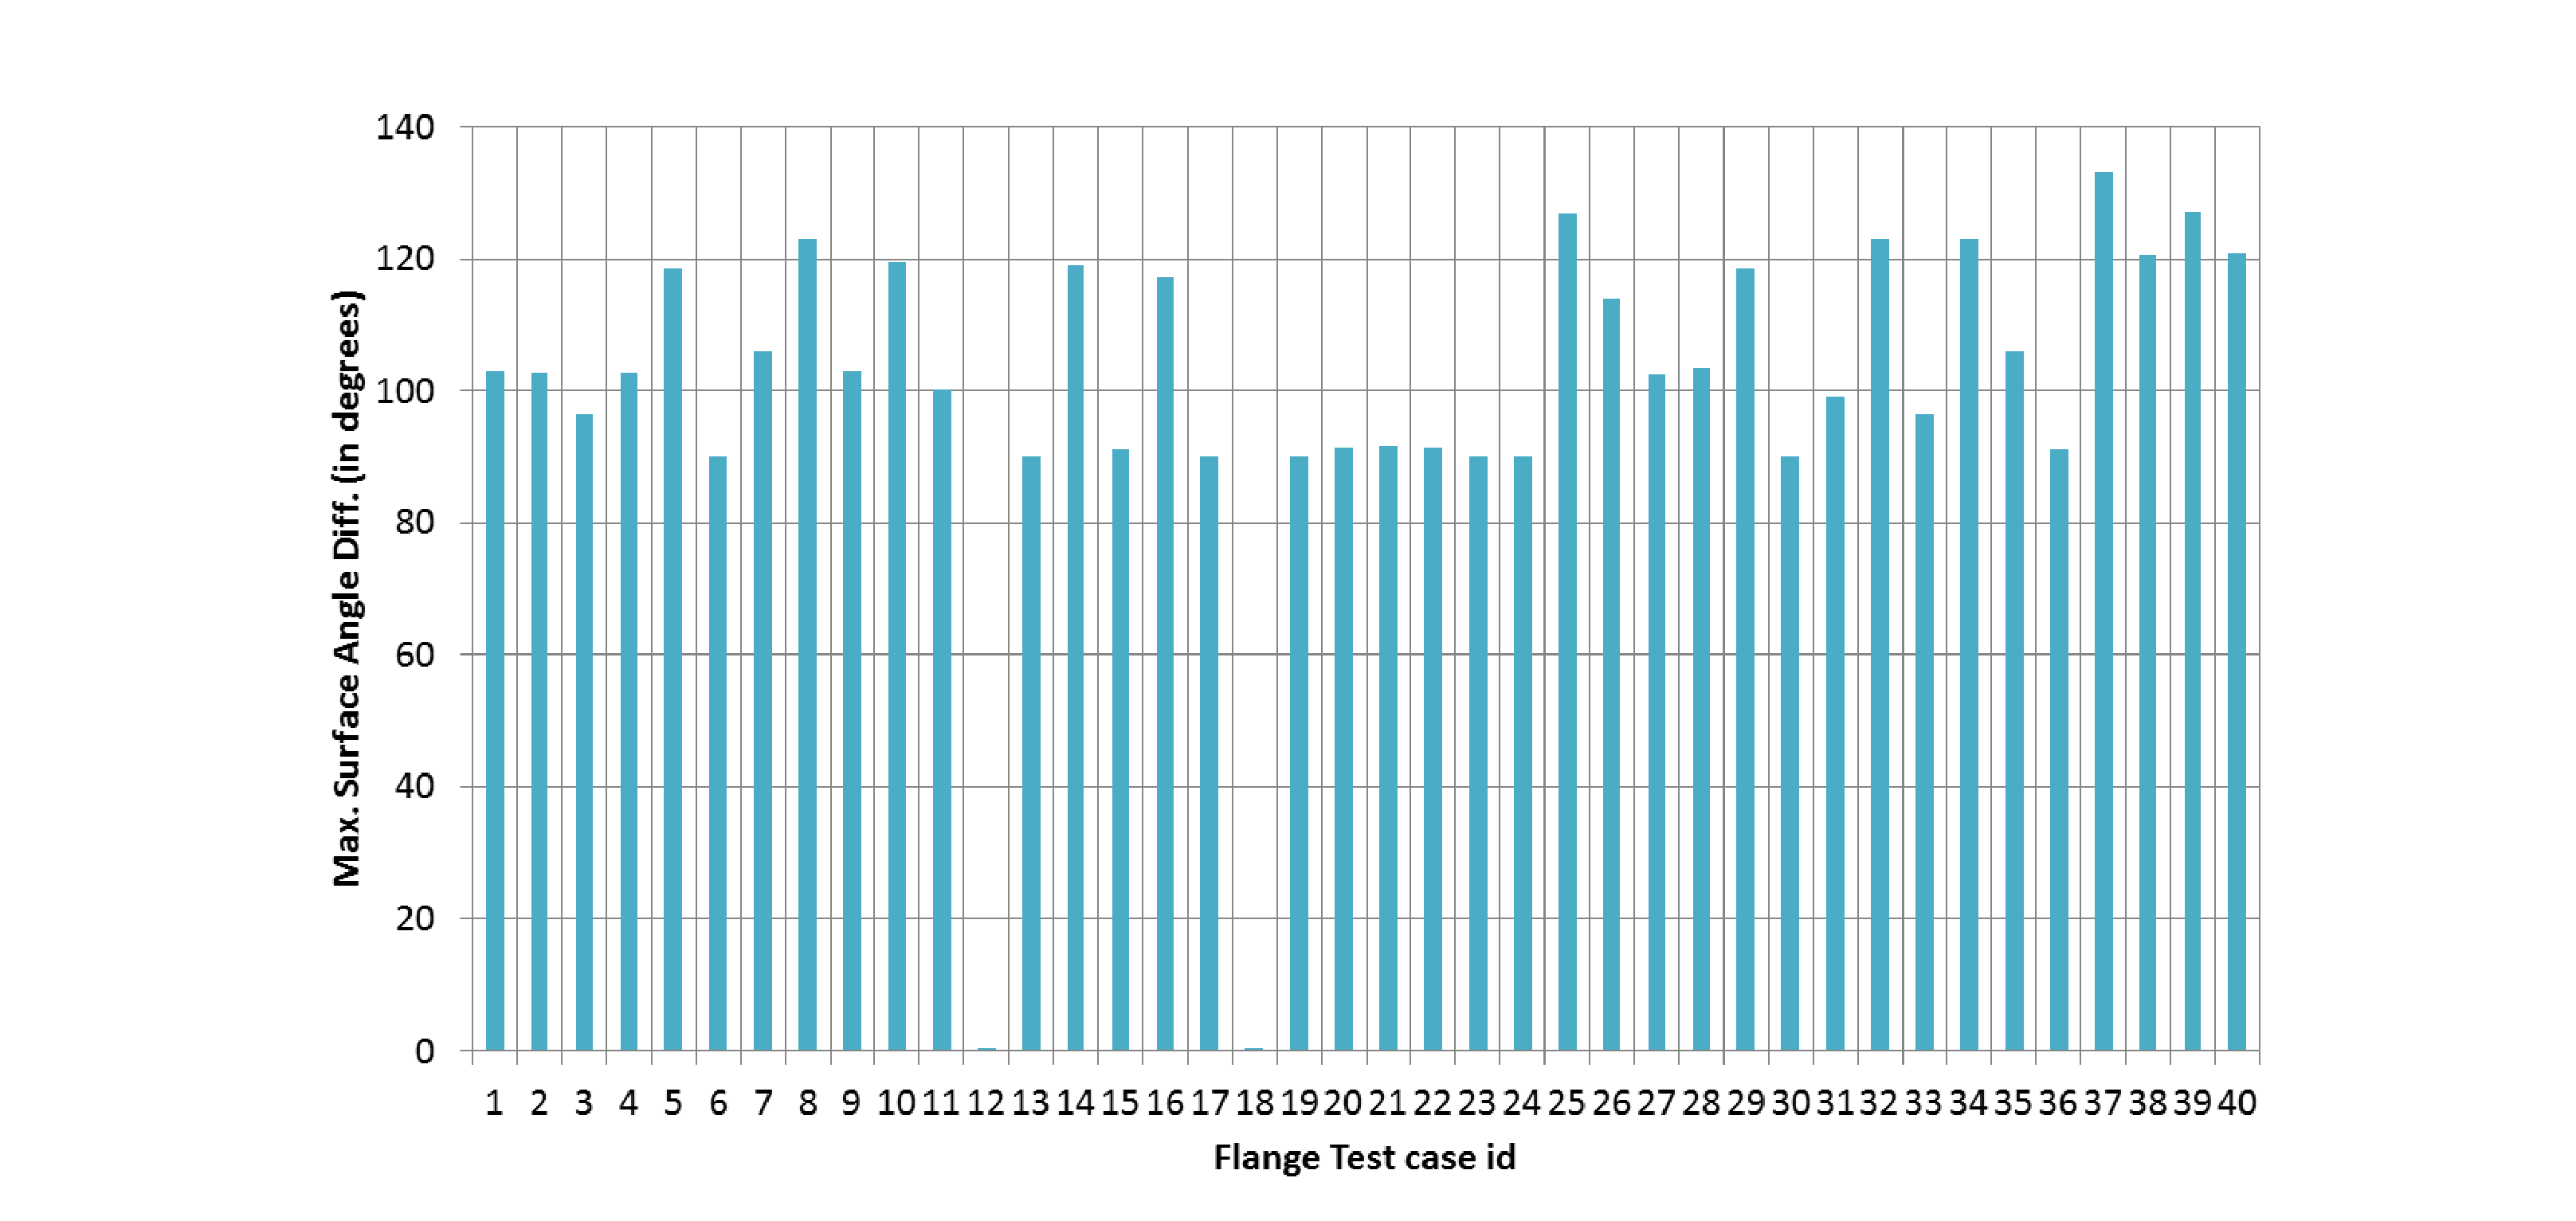
\includegraphics[trim={5cm 0 5cm 0},clip, width=0.45\linewidth]{images/max_surface_angle_Flange.eps}\label{fig:polymender:d}}
				\subfloat[]{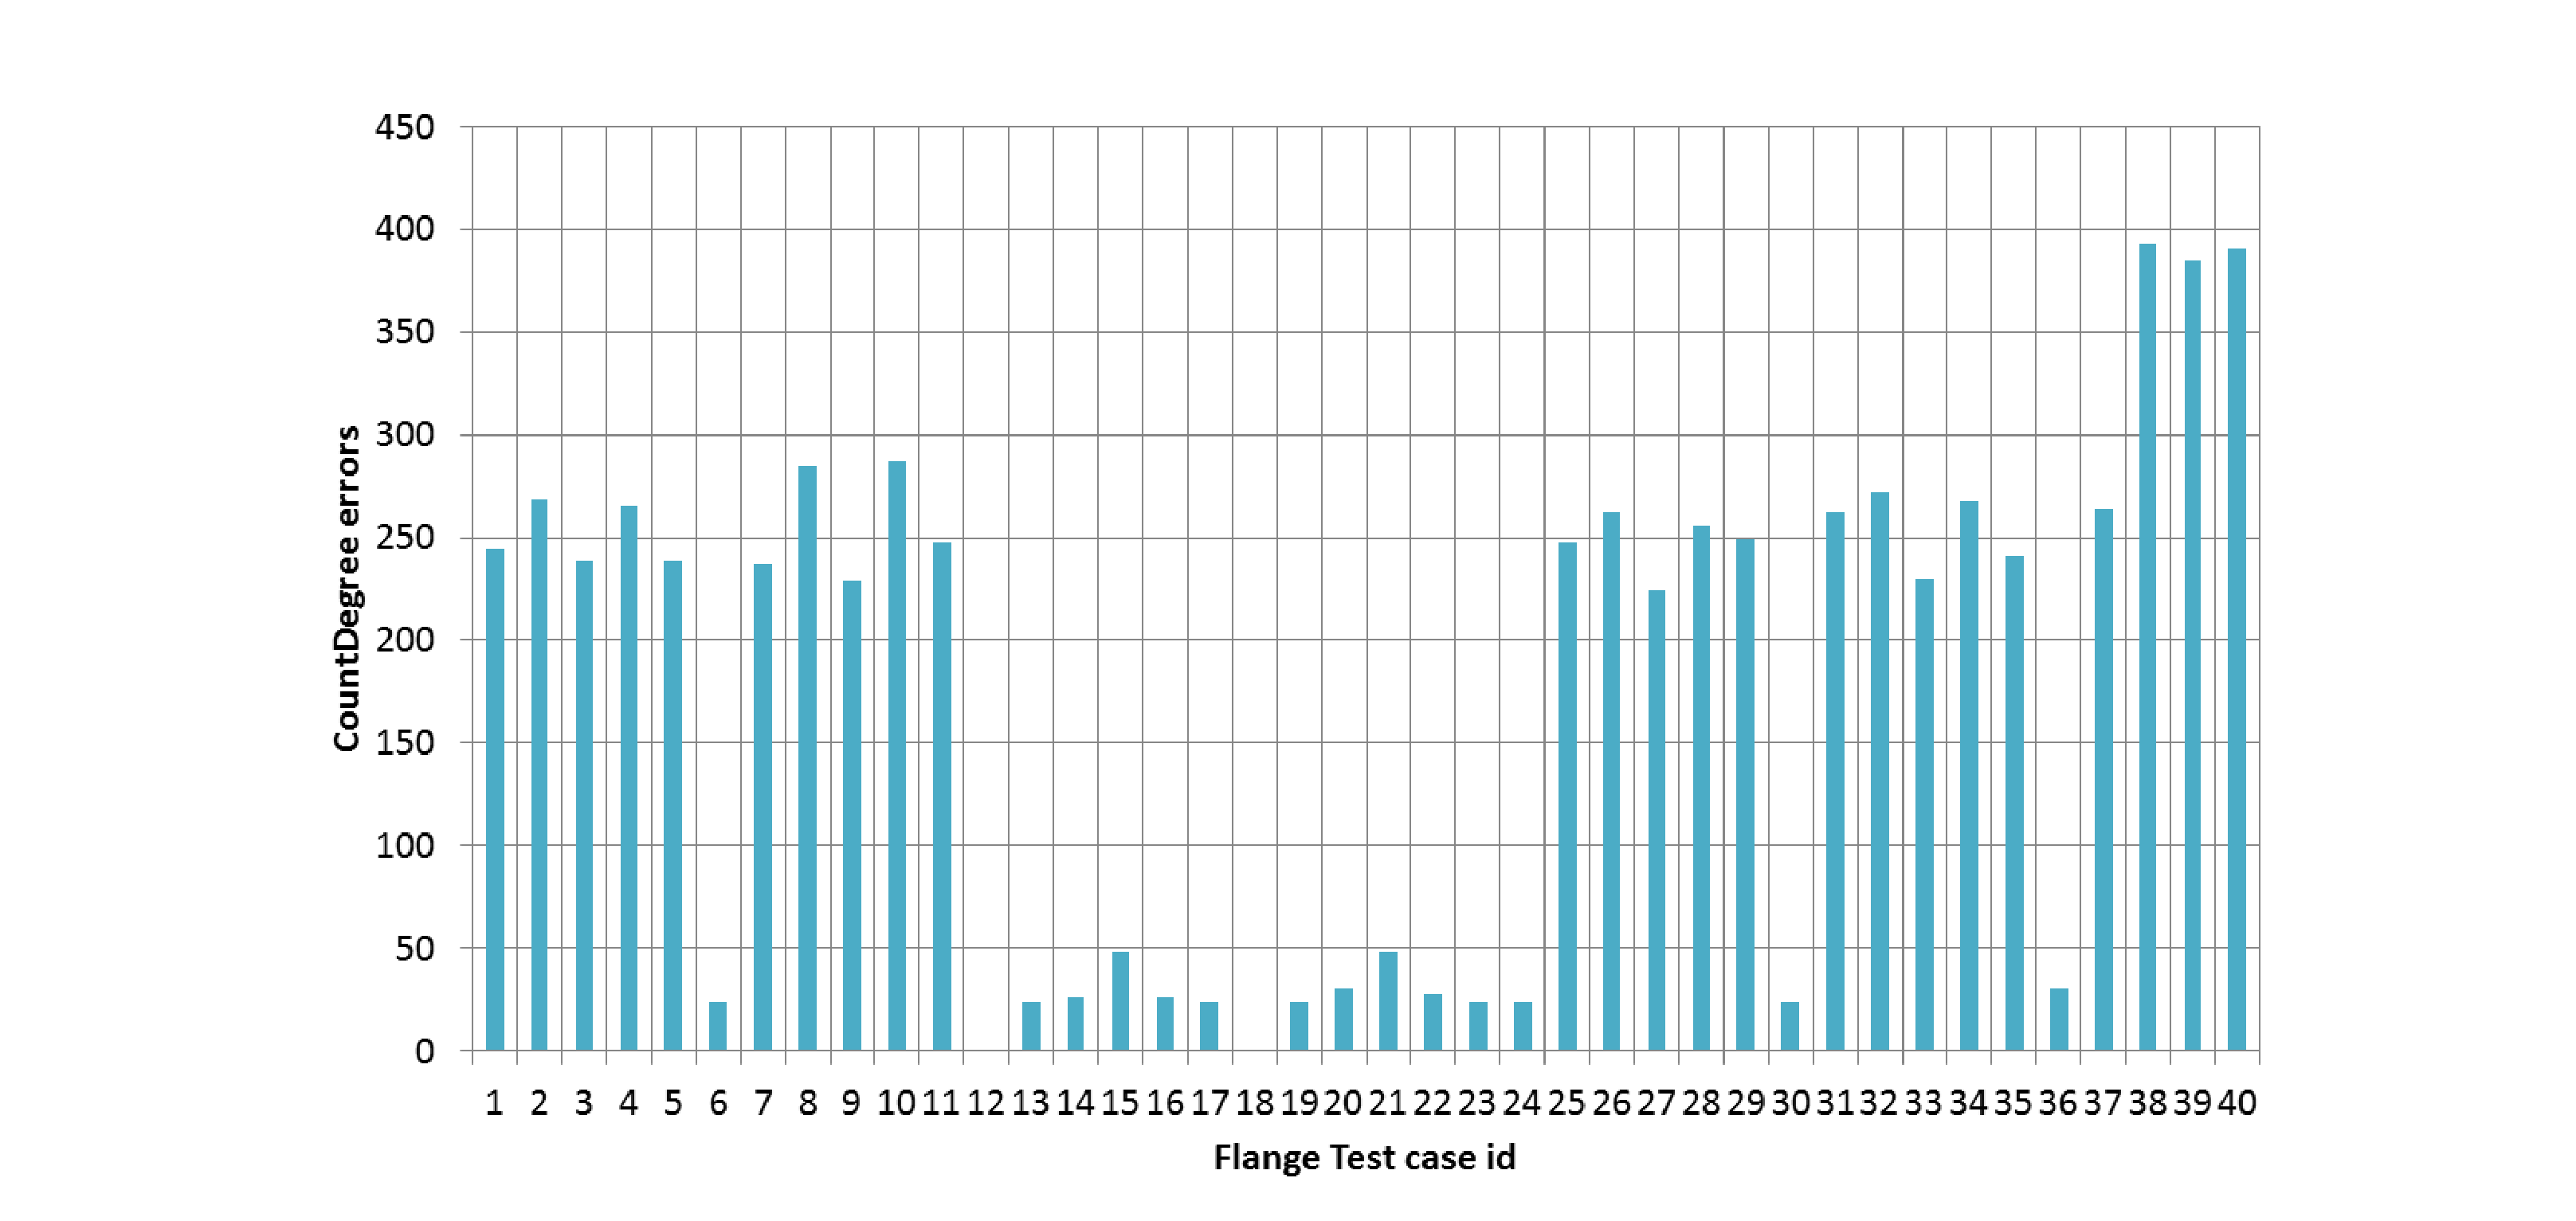
\includegraphics[trim={5cm 0 5cm 0},clip, width=0.45\linewidth]{images/countDegree_Flange.eps}\label{fig:polymender:c}}\\
		\subfloat[]{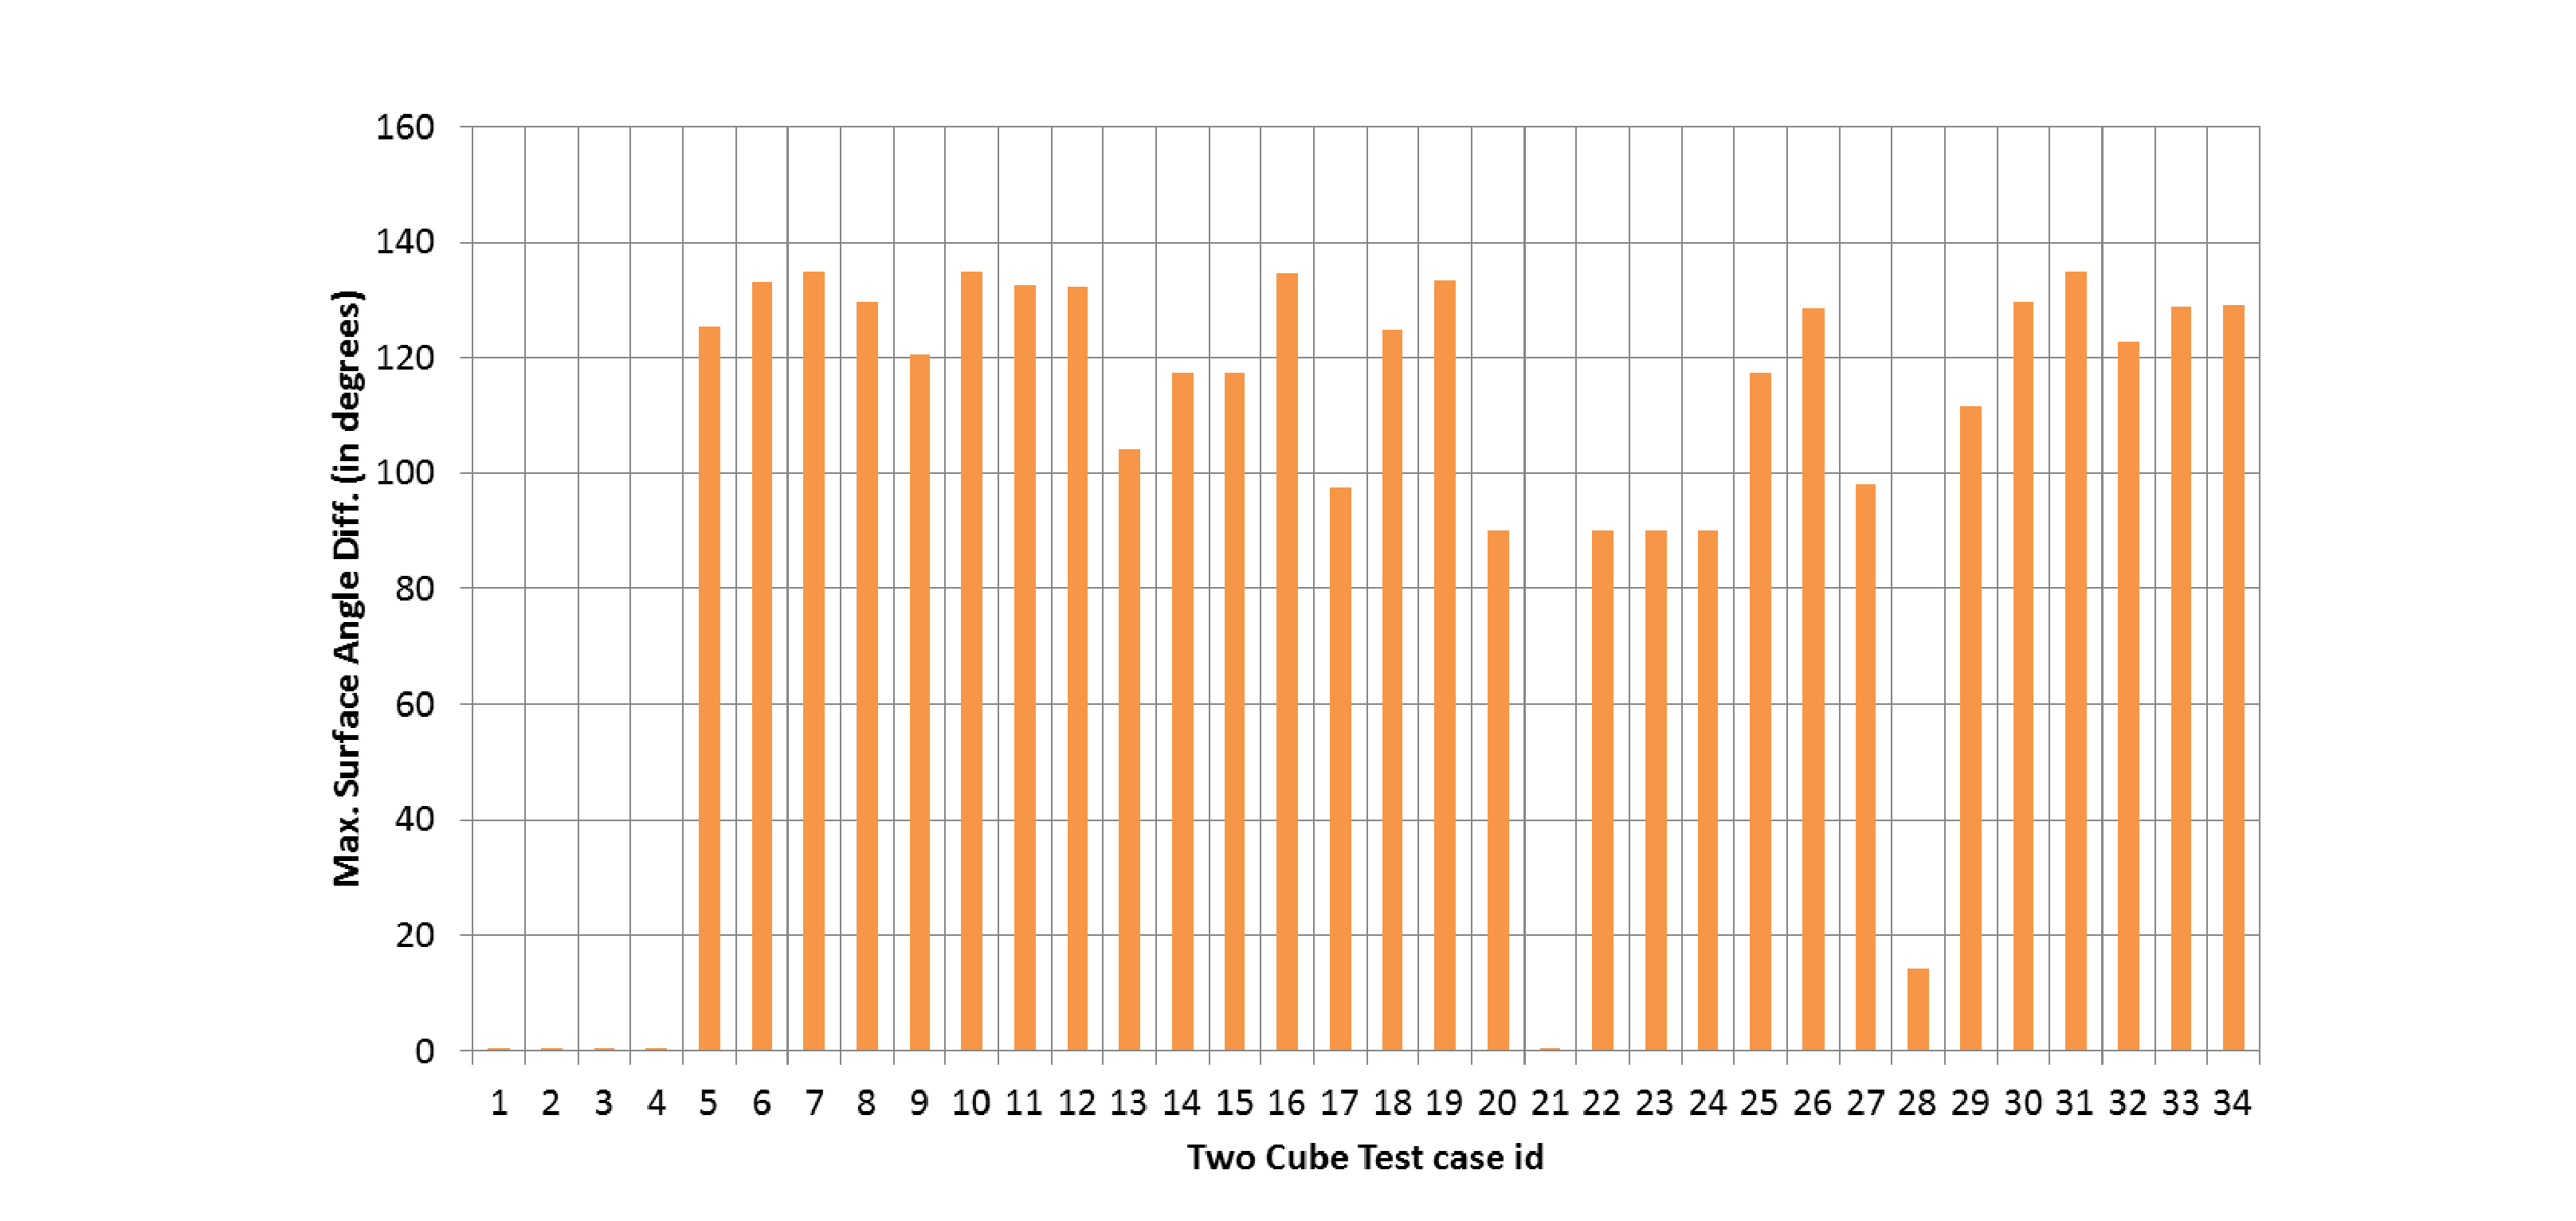
\includegraphics[trim={5cm 0 5cm 0},clip, width=0.45\linewidth]{images/twoCube_summary_1.eps}\label{fig:polymender:b}}\quad
		\subfloat[]{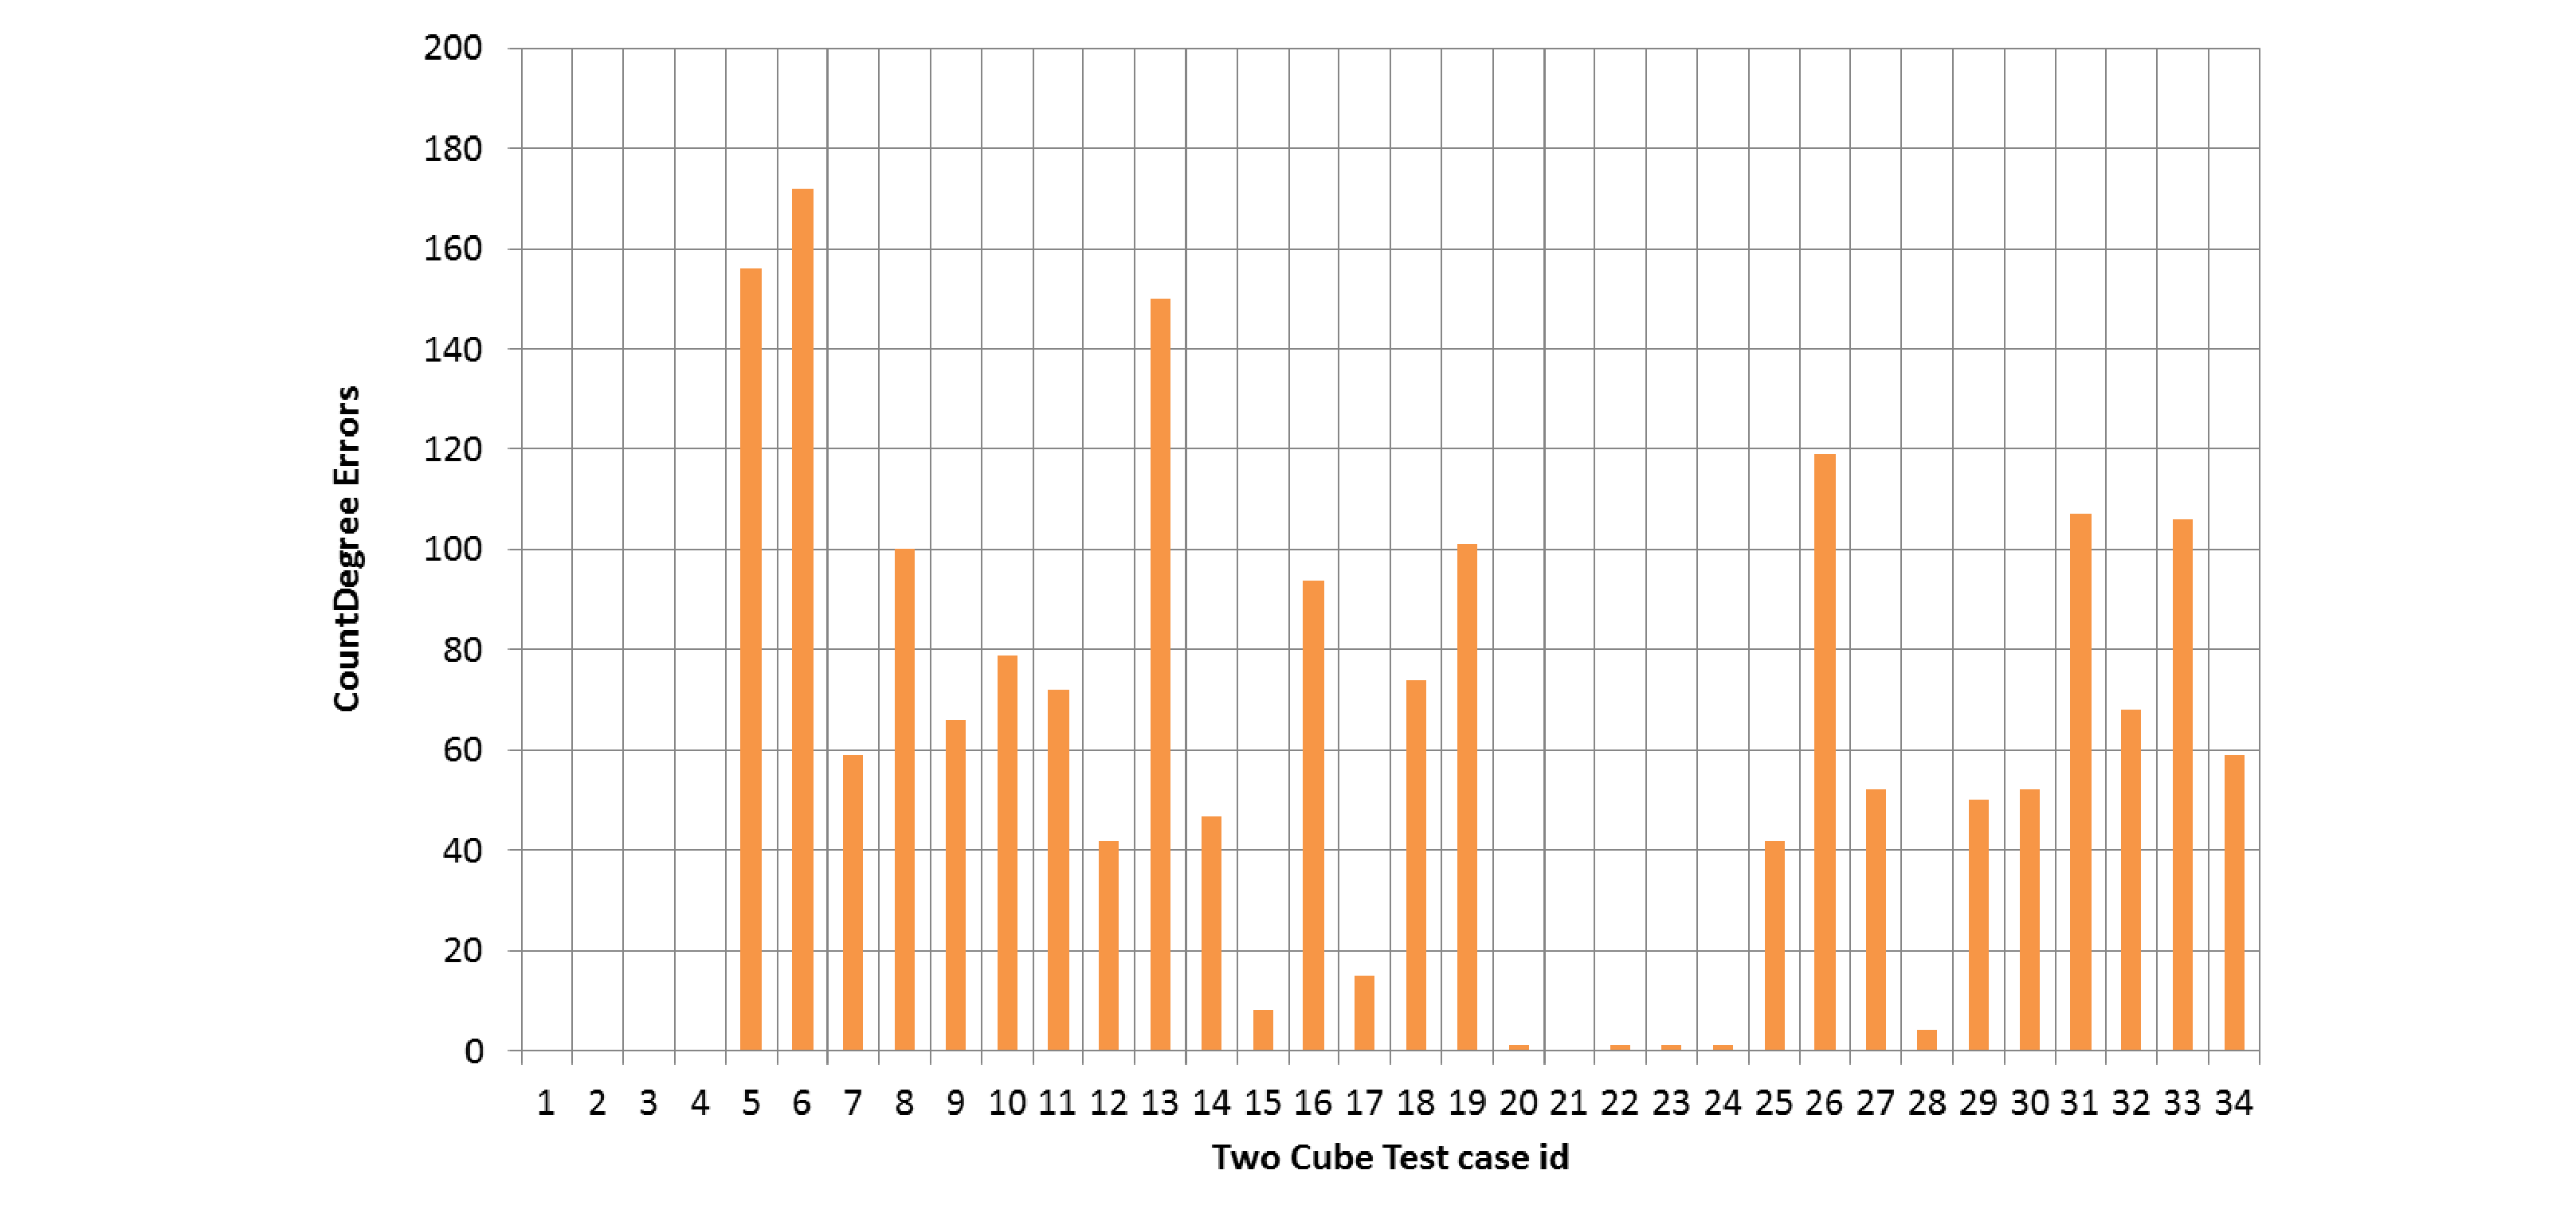
\includegraphics[trim={5cm 0 5cm 0},clip, width=0.45\linewidth]{images/twoCube_summary_2.eps}\label{fig:polymender:a}}\\
		\subfloat[]{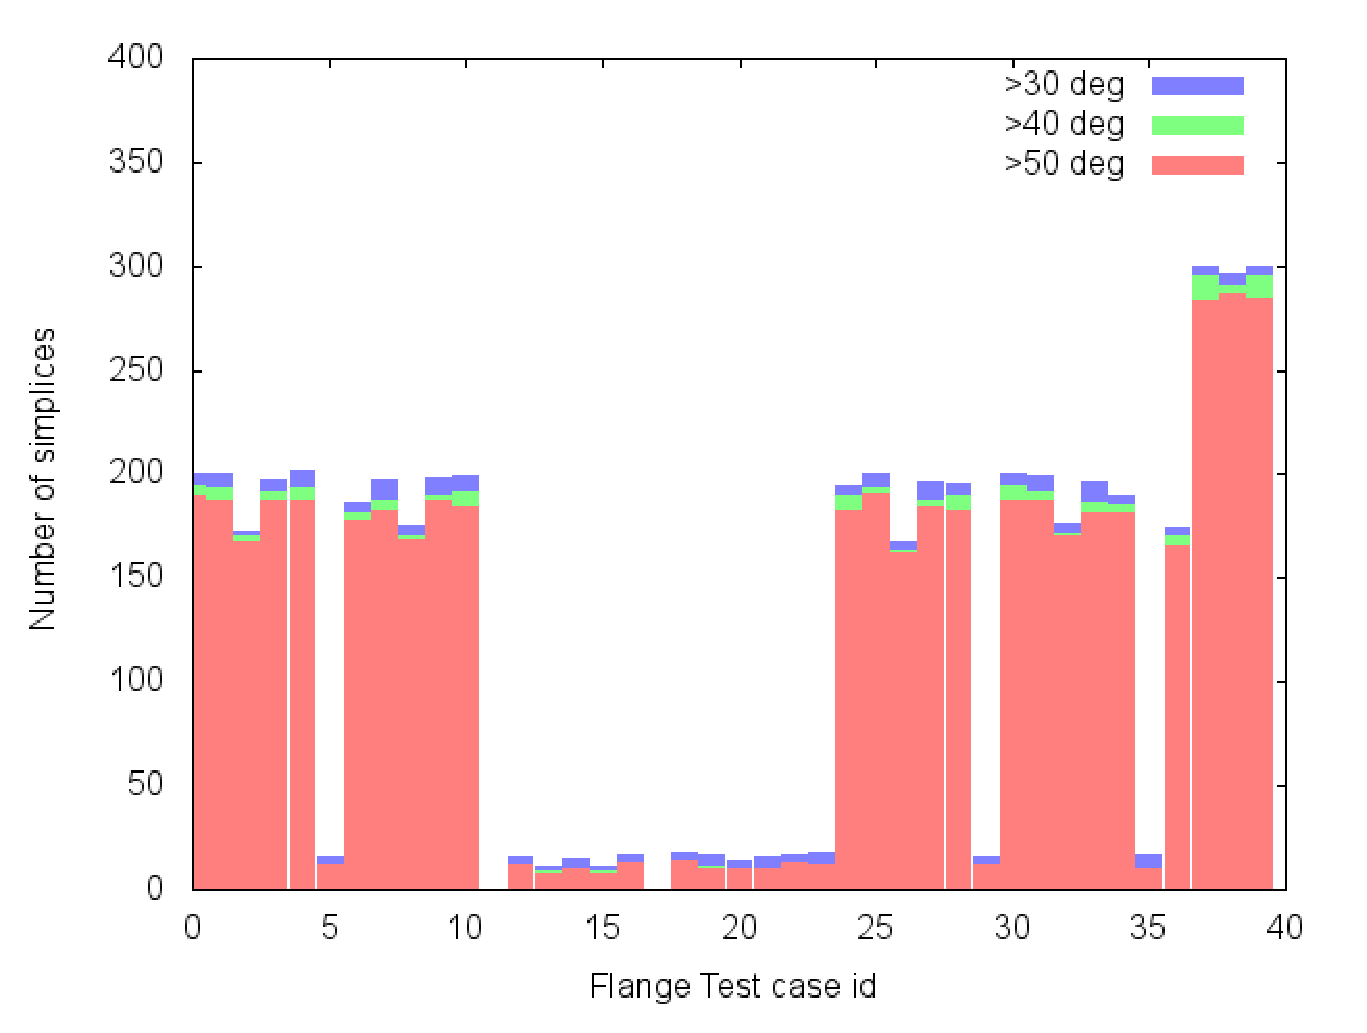
\includegraphics[ width=0.49\linewidth]{images/flange-35-polymender.eps}\label{fig:polymender:e}}
\quad
			\subfloat[]{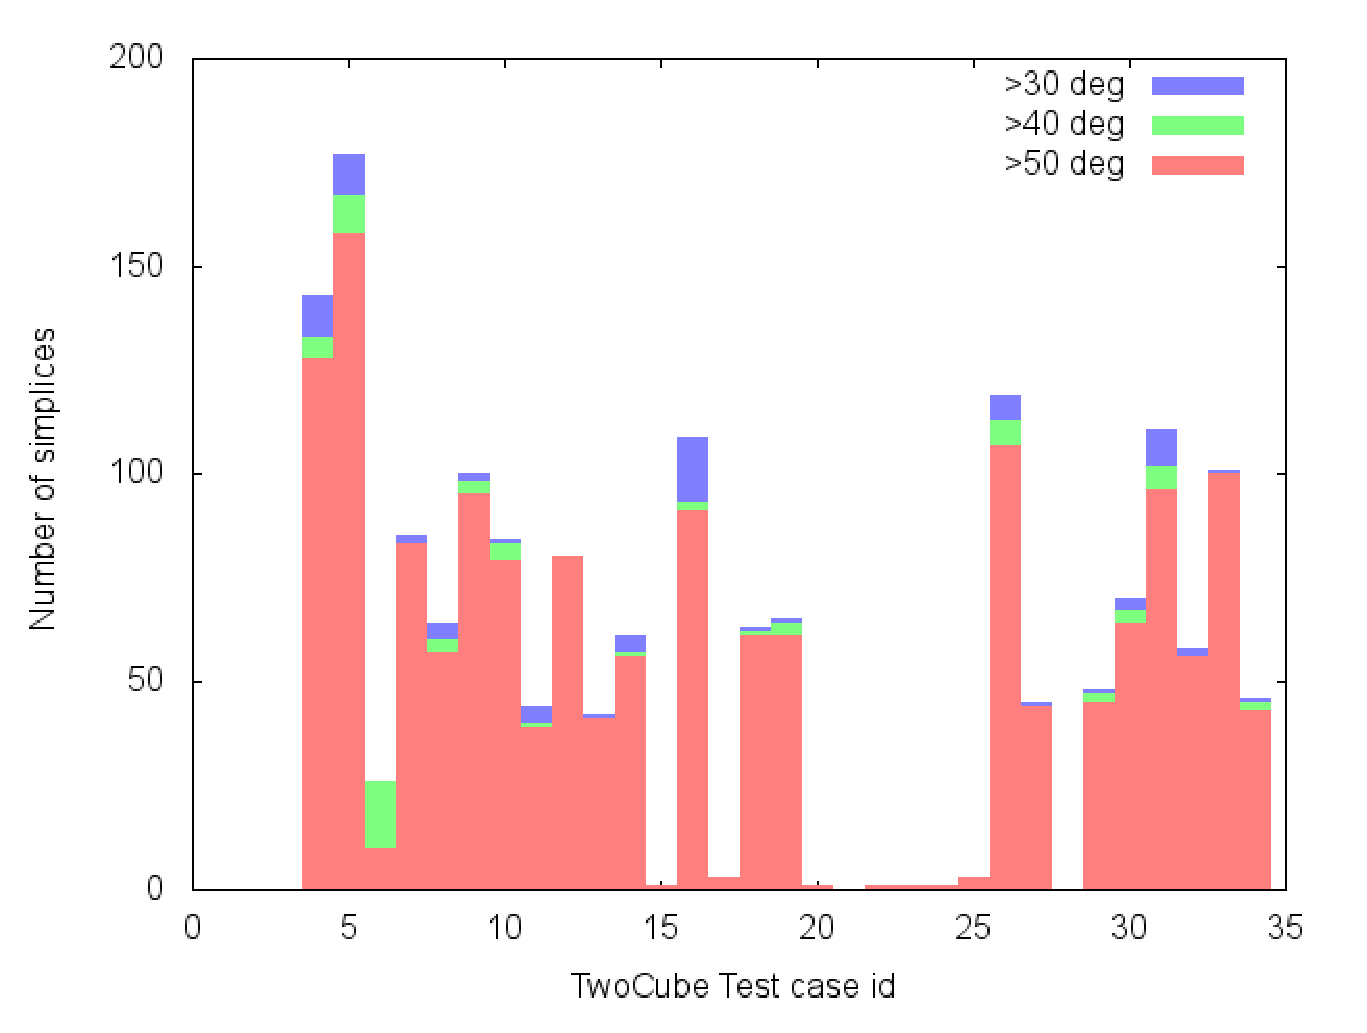
\includegraphics[ width=0.49\linewidth]{images/twocube-35-polymender.eps}\label{fig:polymender:f}}
\\
\caption{Results of PolyMender on 40 Flange and 34 TwoCubes data sets.
\protect\subref{fig:polymender:d}~Oriented angle distance to polygonal Flange meshes.
\protect\subref{fig:polymender:b}~Oriented angle distance to polygonal TwoCubes meshes.
\protect\subref{fig:polymender:c}~Degree errors in 1-skeleton of sharp edges of Flange data sets.
\protect\subref{fig:polymender:a}~Degree errors in 1-skeleton of sharp edges of TwoCubes data sets.
(Note: Y-scale is 0 to 200 compared with y-scale 0 to 450 in (b).)
\protect\subref{fig:polymender:e}~Number of triangles with oriented angle difference to Flange mesh 
above $30$, $40$ and $50$ degrees.
\protect\subref{fig:polymender:f}~Number of triangles with oriented angle difference to TwoCubes mesh
above $30$, $40$ and $50$ degrees.
(Note: Y-scale is 0 to 200 compared with y-scale 0 to 400 in (e).)
}
\label{fig:polymenderA}
\end{figure*}

\paragraph{Comparison with PolyMender.}

PolyMender is an implementation of mesh repairing algorithm from Ju~\cite{j-rrpm-04}.
Input to PolyMender is a set of triangles representing a surface,
but not necessarily properly connected in a polygonal mesh.
PolyMender uses the triangles to build a regular scalar grid
representing the signed distance to the surface.
It also uses the triangles to determine surface normals
on the surface.
It extracts an isosurface mesh using the dual contouring algorithm 
described in~\cite{jlsw-dchd-02,sw-dcss-02}.
The extracted isosurface mesh is the ``mended'' polygonal mesh.

Because PolyMender contains an implementation of the dual contouring algorithm
from~\cite{jlsw-dchd-02,sw-dcss-02},
we used it to compare SHREC and the algorithm from~\cite{jlsw-dchd-02,sw-dcss-02}.
Our inputs to PolyMender were the polygonal meshes
(Figure~\ref{fig:mesh})
designed specifically for each surface to accurately represent the 0-dimensional
and 1-dimensional features on the surface.

PolyMender builds a multiresolution isosurface
using an octree instead of a fixed regular grid.
The highest resolution is determined by the depth of the octree.
For all tests, we ran PolyMender with octree depth set of 7.
At the highest resolution,
this octree sampled data from a regular grid with dimensions $\gDim{2^7}$ or $\gDim{128}$.
We set the scale set to 0.9 and used defaults for all other parameters.

Figures~\protect\subref*{fig:polymenderB:b} and~\protect\subref*{fig:polymenderB:a} 
show part of a Flange isosurface reconstructed by PolyMender
and a corresponding isosurface produced by SHREC (Religrad gradients).
Note the flipped triangles and distorted ``sharp'' curve (red) in the PolyMender isosurface.
Figure~\protect\subref*{fig:polymenderB:c} shows the distribution of differences 
of triangle normals between the PolyMender isosurface and the polyhedral mesh
and between the SHREC isosurface and the polyhedral mesh.
All SHREC triangle normals are within $25^\circ$ of the polyhedral mesh normals,
while PolyMender has numerous triangles with normals greater than $30^\circ$
of the polyhedral mesh normals.

Figures~\subref*{fig:polymender:cone:b}, \subref*{fig:polymender:cone:a}
and~\subref*{fig:polymender:cone:c}
show a PolyMender Smooth Tip Cone isosurface and 
the corresponding SHREC isosurface (Religrad gradients).
The 1-dimensonal feature around the base of the cone has a $60^\circ$ dihedral angle.
In the PolyMender isosurface,
there are numerous ``notches'' along the 1-dimensional feature.

We ran PolyMender on the same 40 Flange and 34 TwoCube meshes
that we applied to SHREC in Section~\ref{section:synthetic_tests}.
Figure~\ref{fig:polymenderA} shows the oriented angle distances from the polygonal meshes
and the degree errors in the 1-skeletons of sharp edges.
Most of the PolyMender Flange and TwoCubes isosurfaces had an oriented angle distance greater than $90^\circ$
from the corresponding polygonal meshes.
24 out of 40 of the PolyMender Flange isosurfaces had over 150 triangles
whose normals were more than $50^\circ$ from the normals of the corresponding polygonal meshes.
In comparison, only one SHREC Flange isosurface (Religrad gradients) had triangles
whose normals were more than $50^\circ$ from the normals of the corresponding polygonal meshes
(Figure~\ref{fig:flangeAngle}).
No SHREC Flange isosurface (Religrad gradients) had more than 15 triangles
whose normals were more than $30^\circ$ from the normals of the corresponding polygonal meshes
Almost all of the PolyMender Flange isosurfaces had degree errors
and 25 out of 40 had over 200 degree errors.
Only 8 out of 40 SHREC Flange isosurfaces (Religrad gradients) had degree errors
and the maximum number of degree errors was eight.

PolyMender did a bit better on the TwoCubes isosurfaces,
probably because the 1-dimensional features in the TwoCubes level sets are line segments.
Only one of the 34 PolyMender TwoCubes isosurfaces had over 150 triangles
whose normals were more than $50^\circ$ from the normals of the corresponding polygonal meshes.
18 out of 34 PolyMender TwoCubes isosurfaces had over 50 triangles
whose normals were more than $50^\circ$ from the normals of the corresponding polygonal meshes.
Most of the PolyMender TwoCubes isosurfaces had degree errors,
but none had more than 180 degree errors.
8 out of 34 had more than 100 degree errors
and 22 out of 34 had more than 40 degree errors.
5 out of 34 SHREC TwoCubes isosurfaces (Religrad gradients)
had angle distance greater than $40^\circ$ to the corresponding polygonal meshes.
The same five SHREC isosurfaces had degree errors,
but no SHREC isosurface had more than four such errors.

\begin{figure*}
	\centering
	\subfloat[]{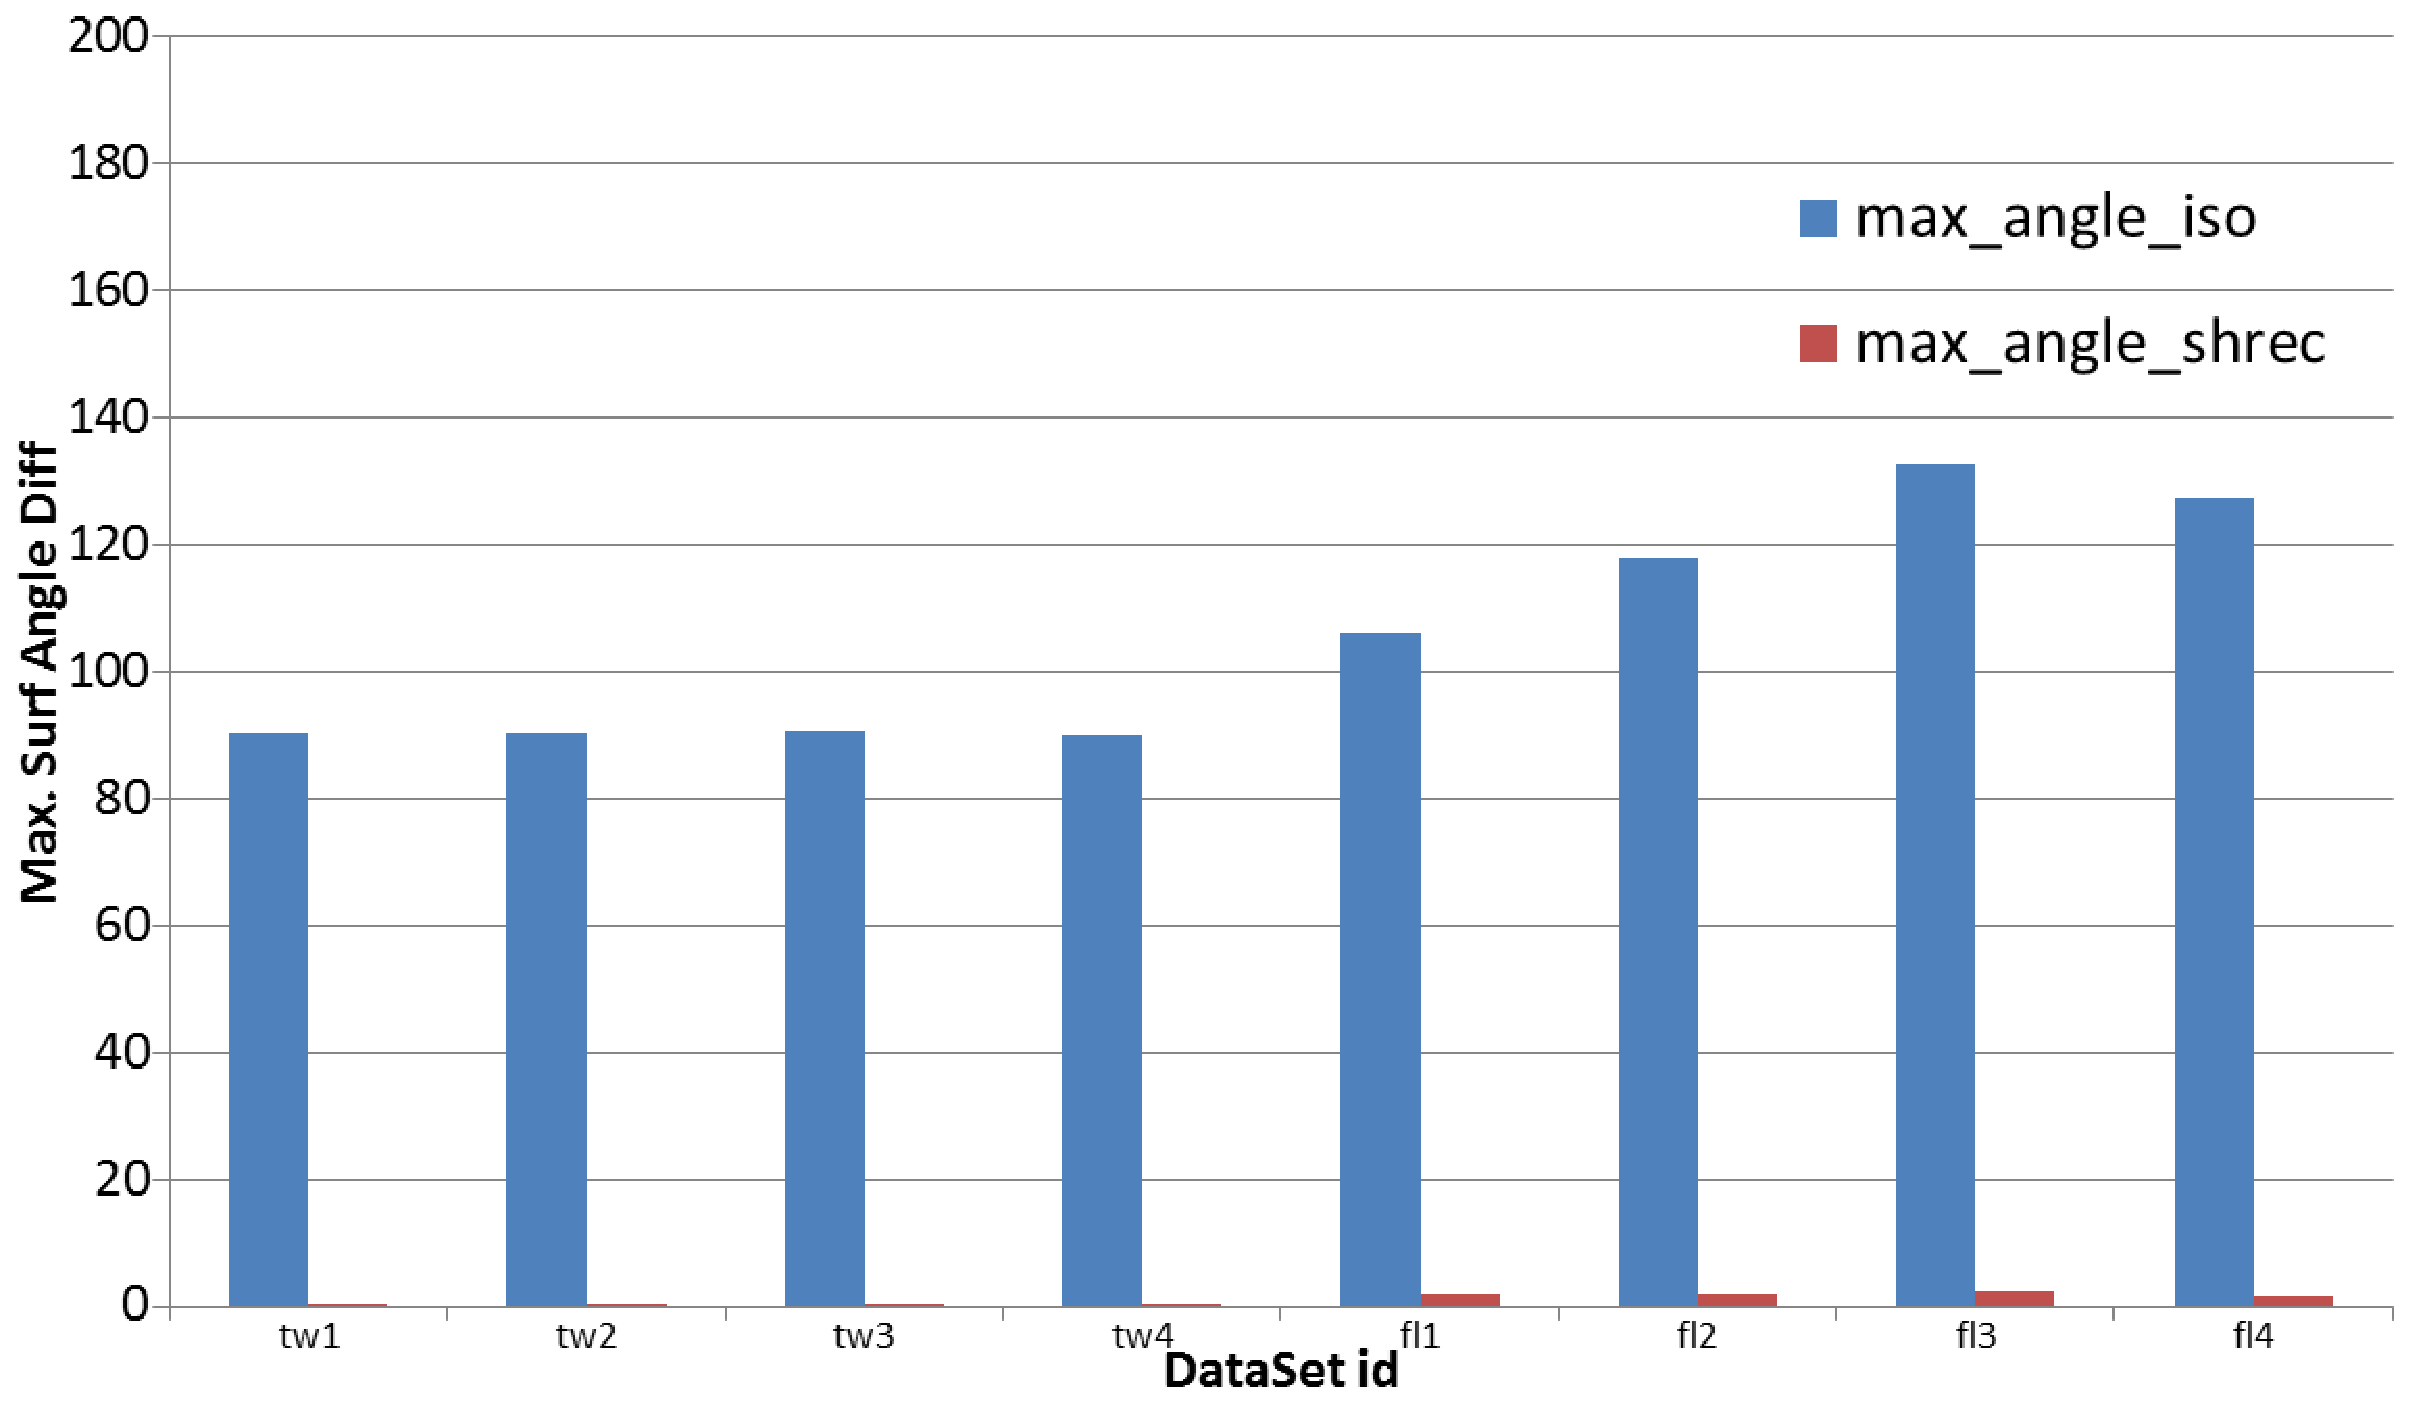
\includegraphics[height=0.2\linewidth]{images/max_angle_isoex_2.eps}\label{fig:isoEx_summ:b}}
	\subfloat[]{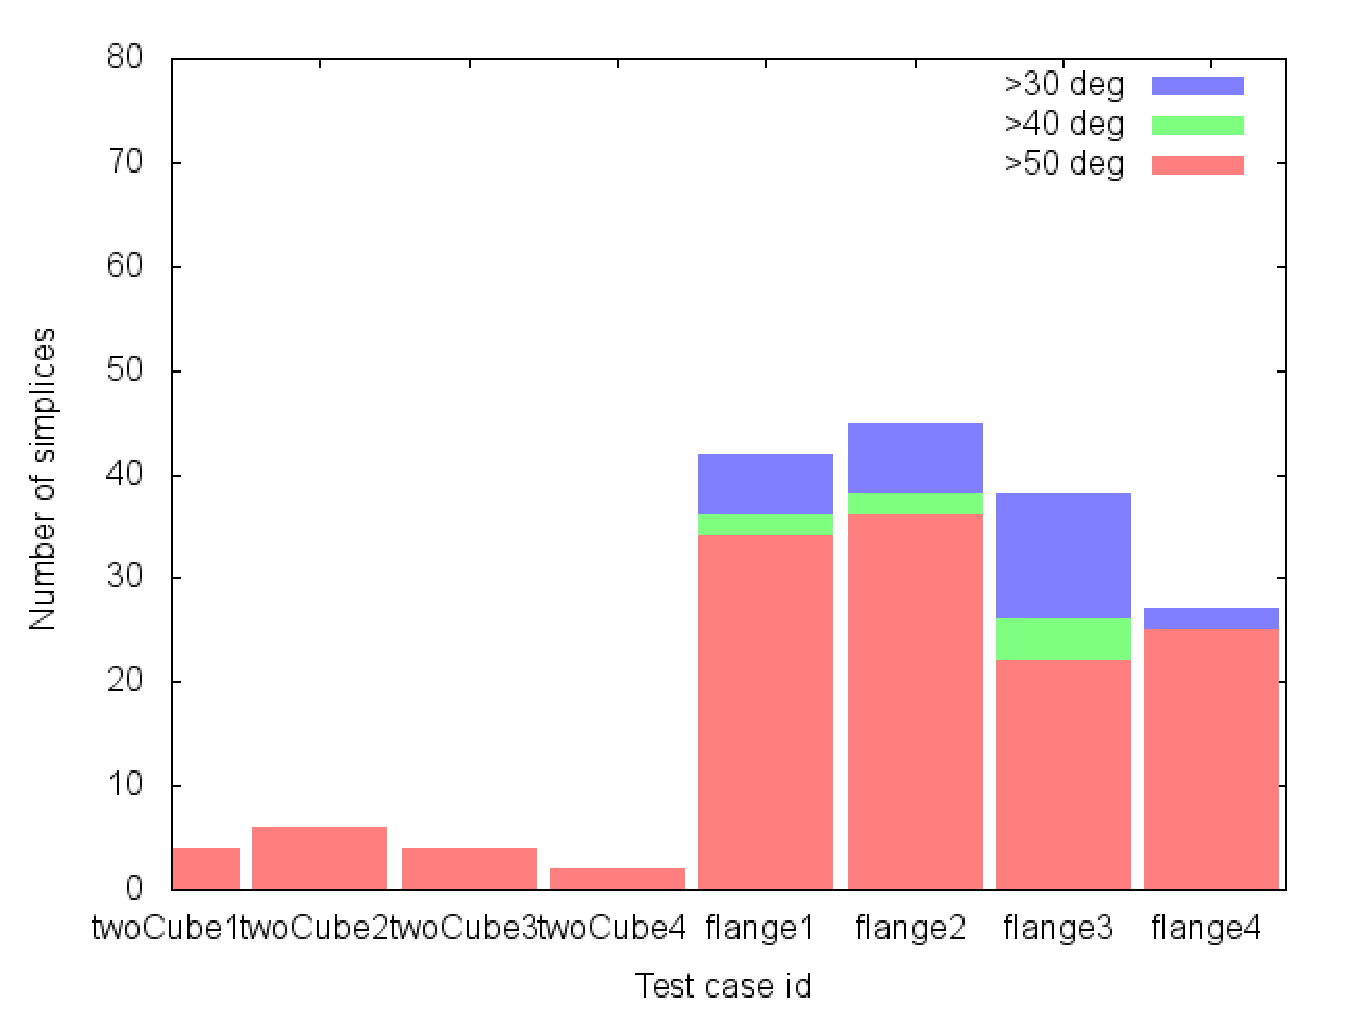
\includegraphics[height=0.2\linewidth]{images/isoex_surf_angle_dist.eps}\label{fig:isoEx_summ:c}}
	\subfloat[]{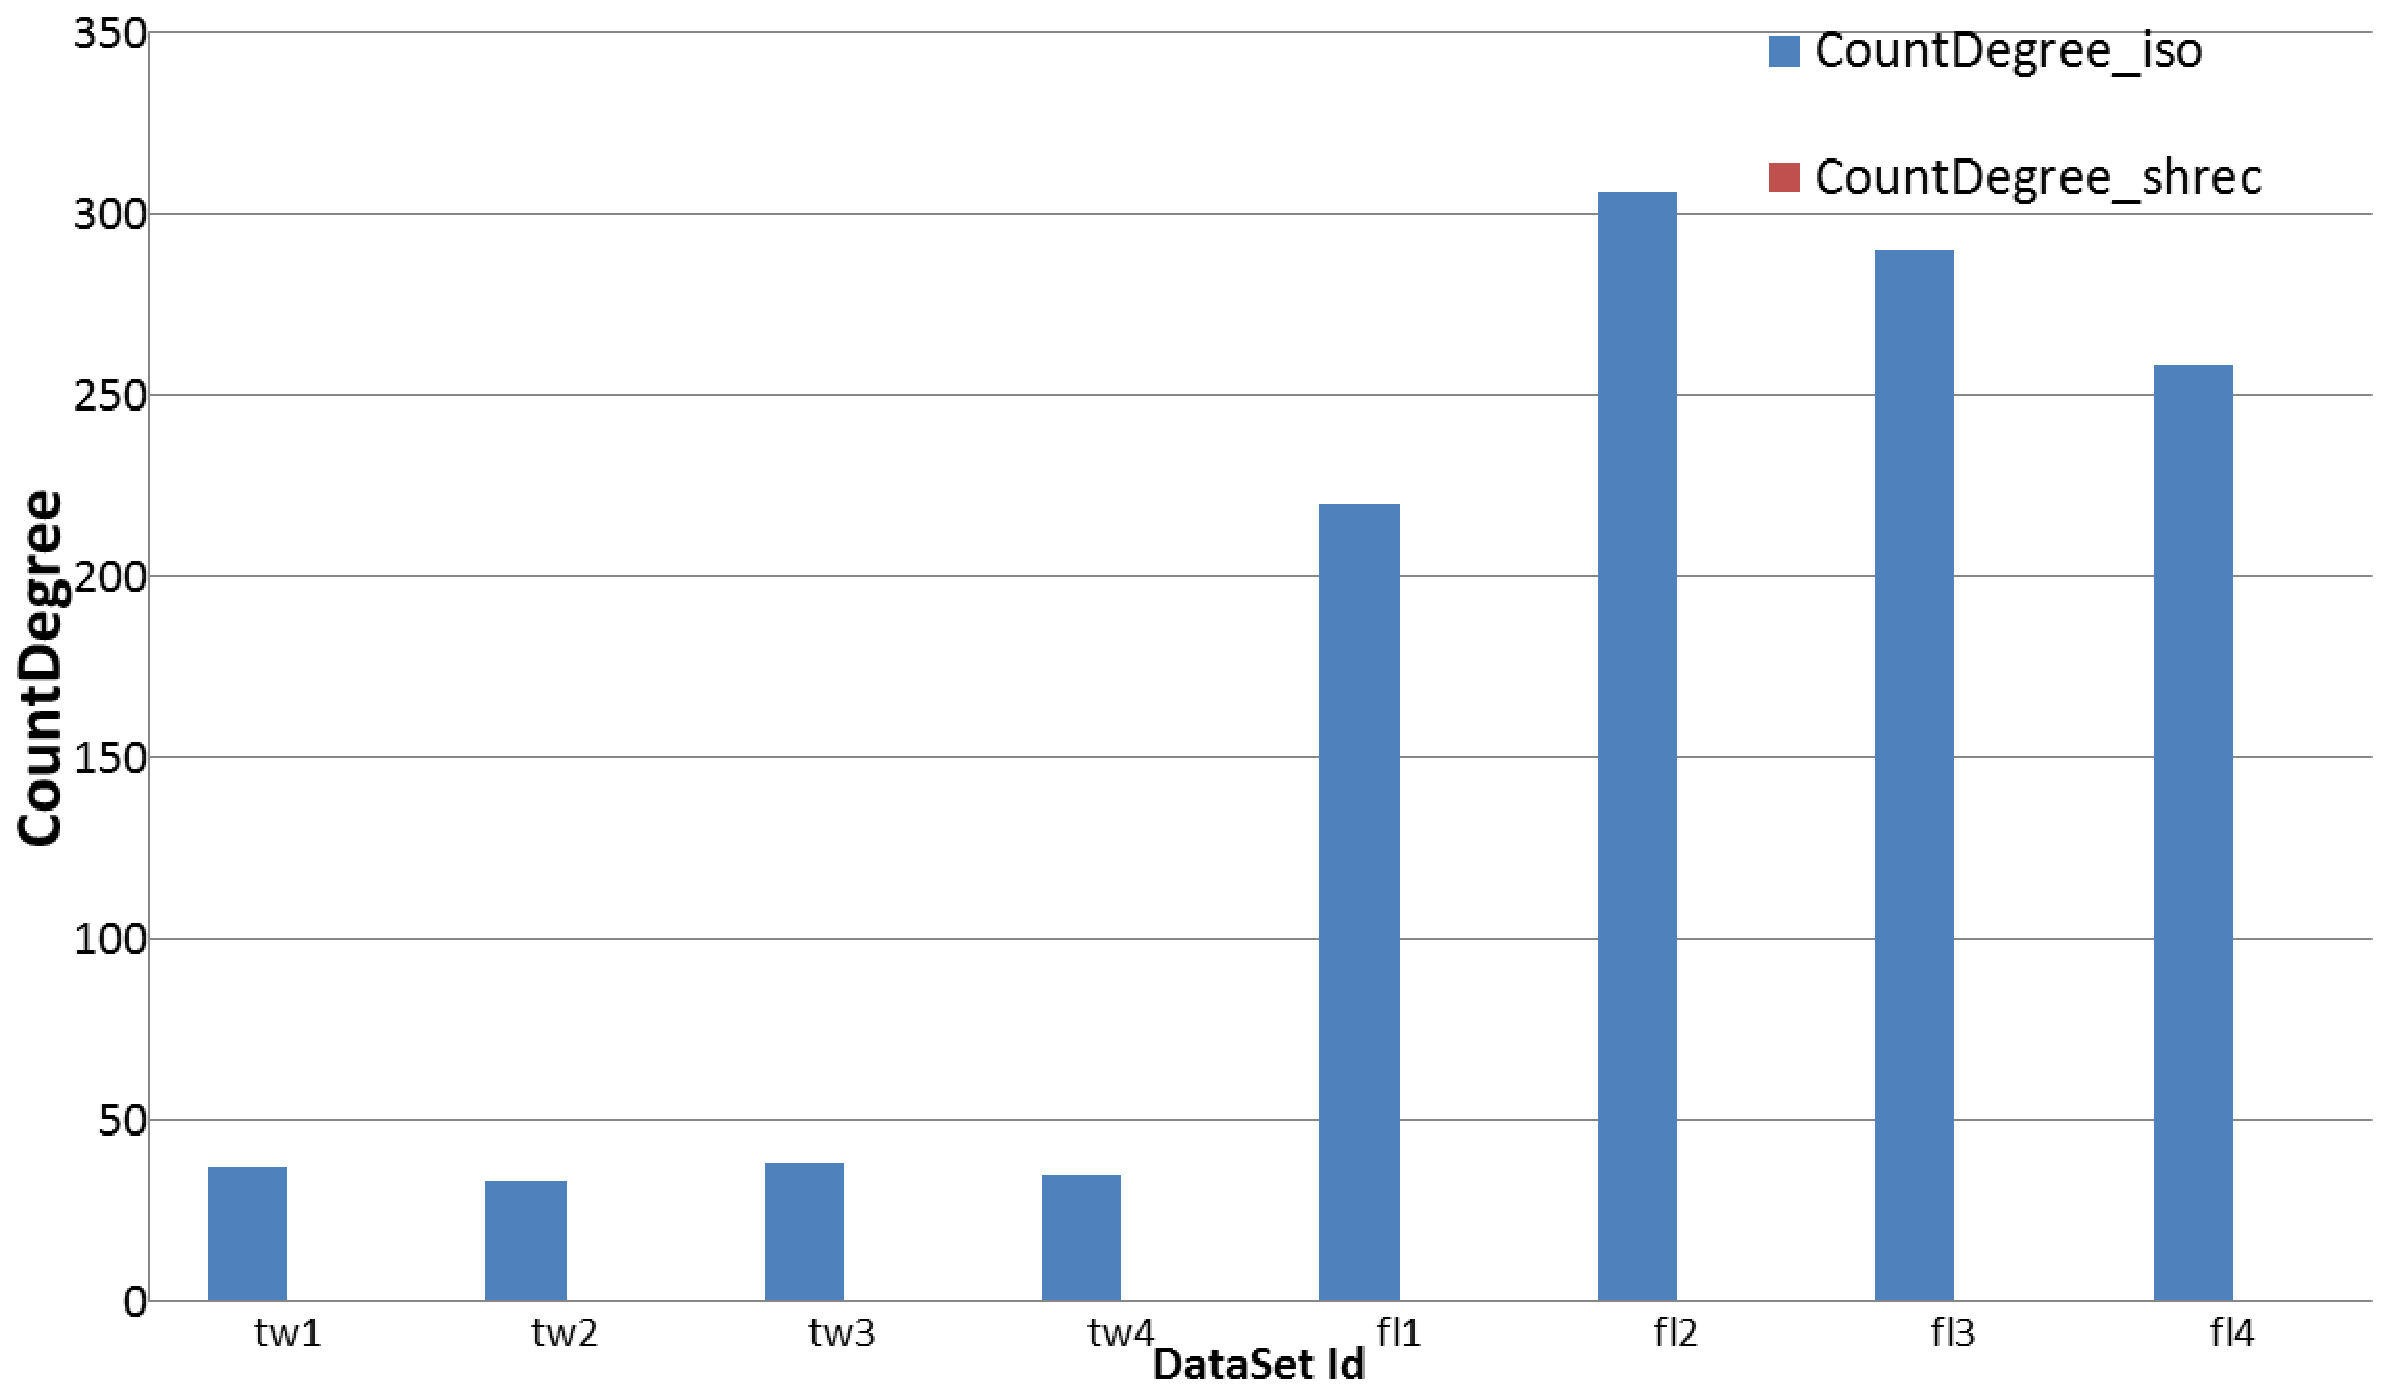
\includegraphics[height=0.2\linewidth]{images/countDegree_isoex_2.eps}\label{fig:isoEx_summ:a}}\\
	\subfloat[]{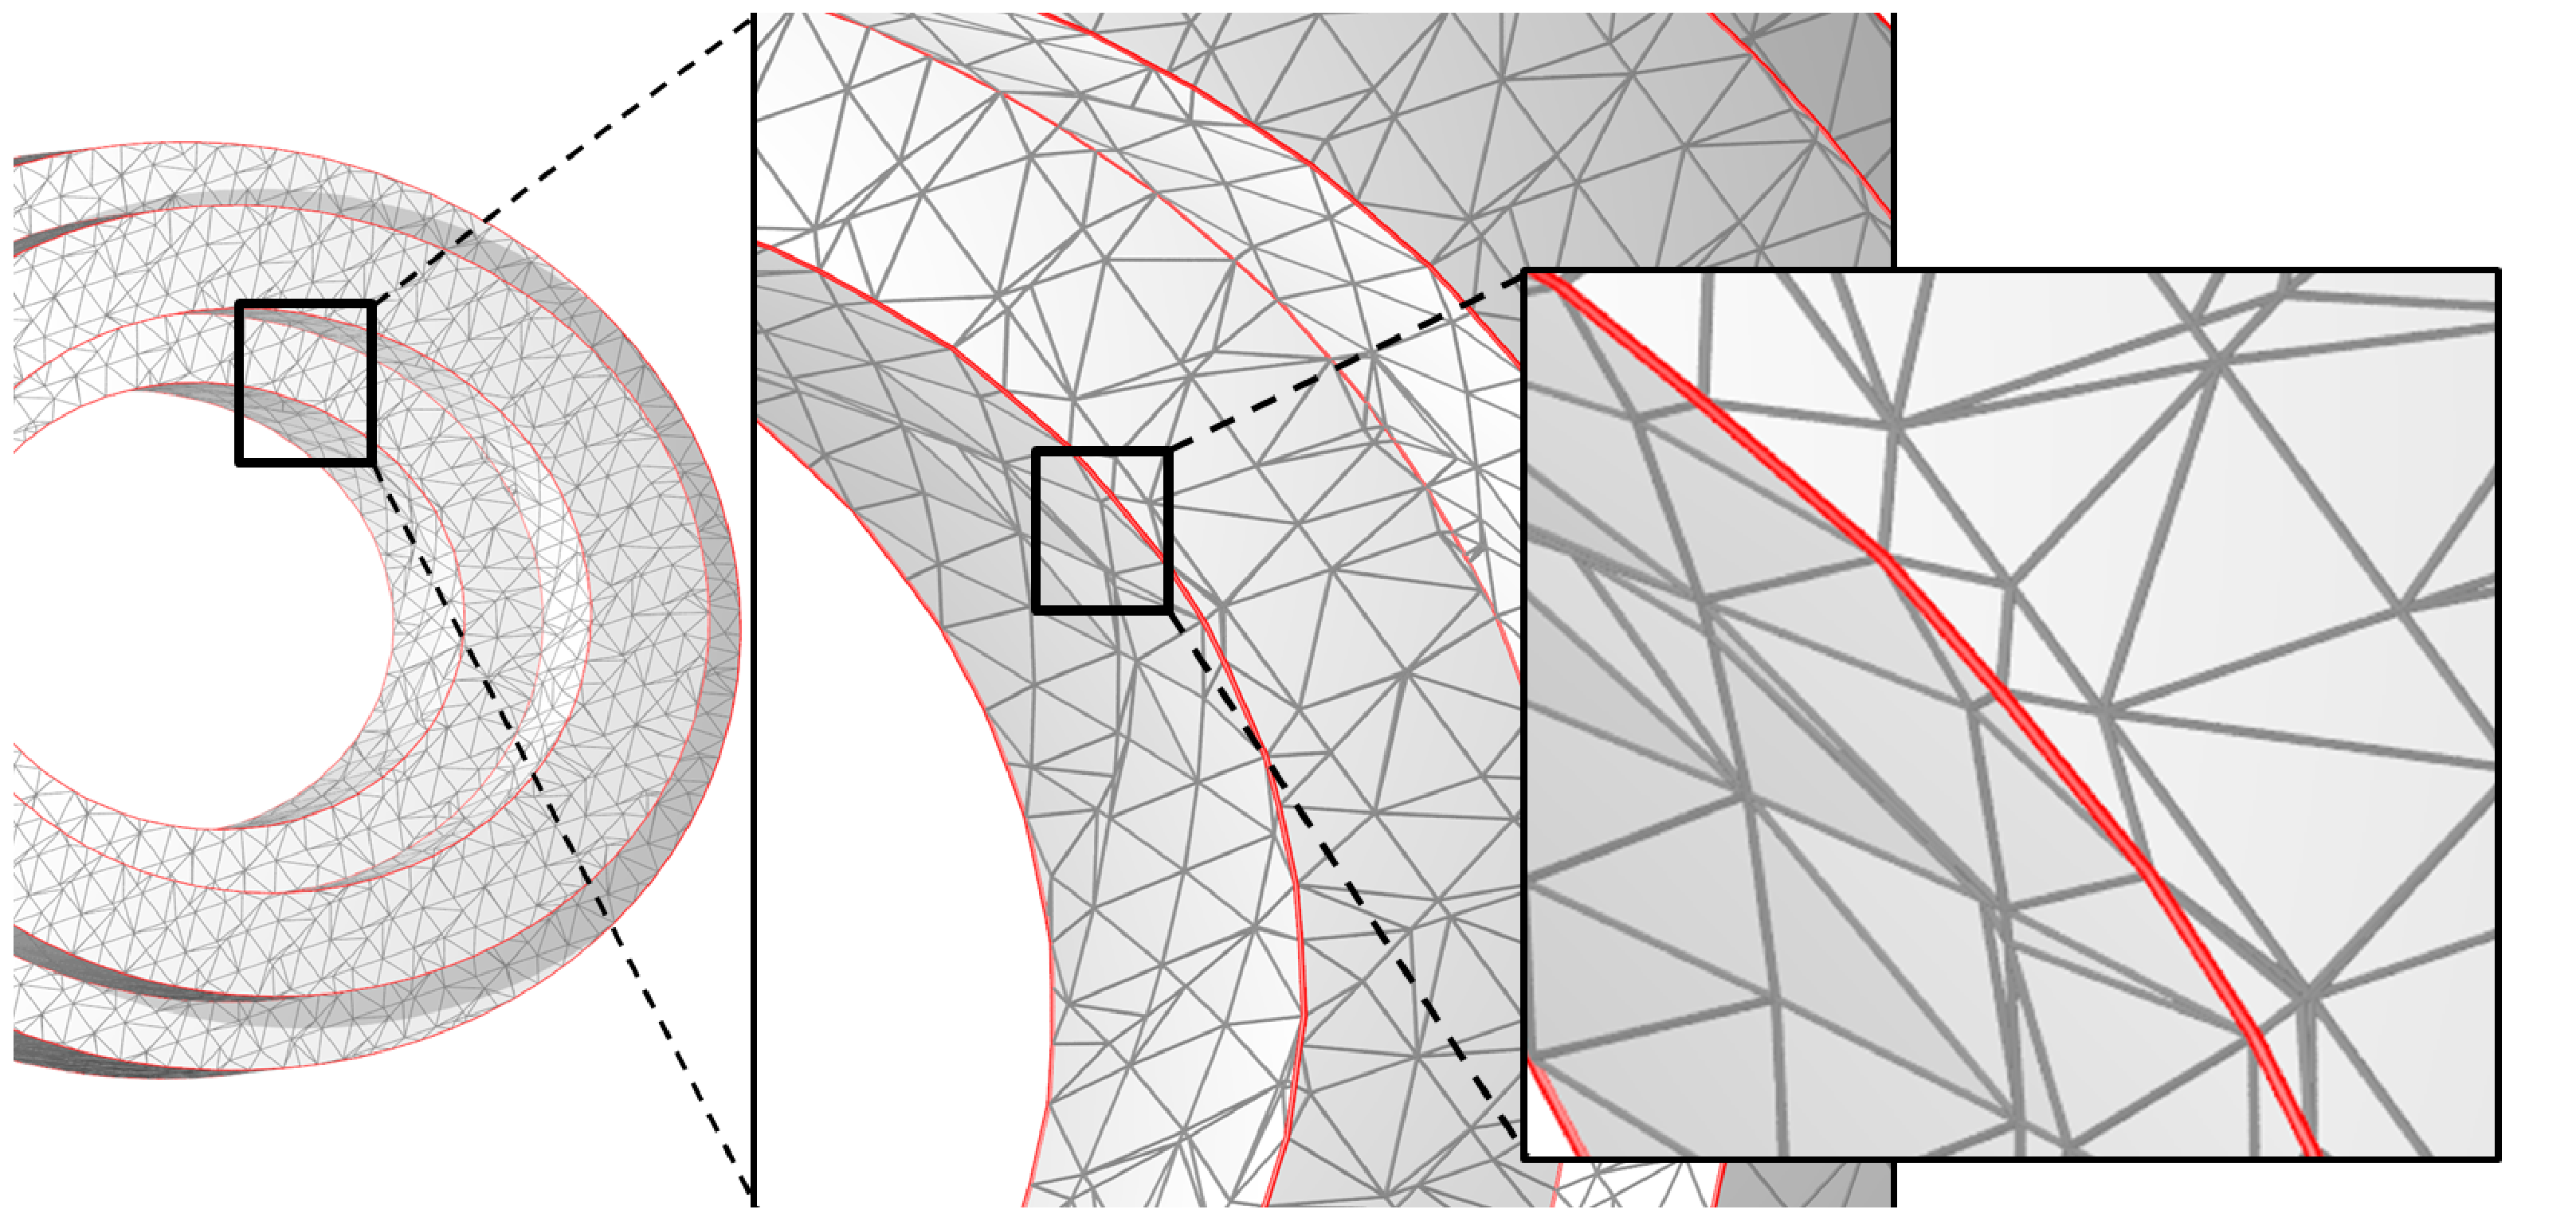
\includegraphics[width=0.5\linewidth]{images/isoExFlange.eps}\label{fig:isoEx:a}}
	\subfloat[]{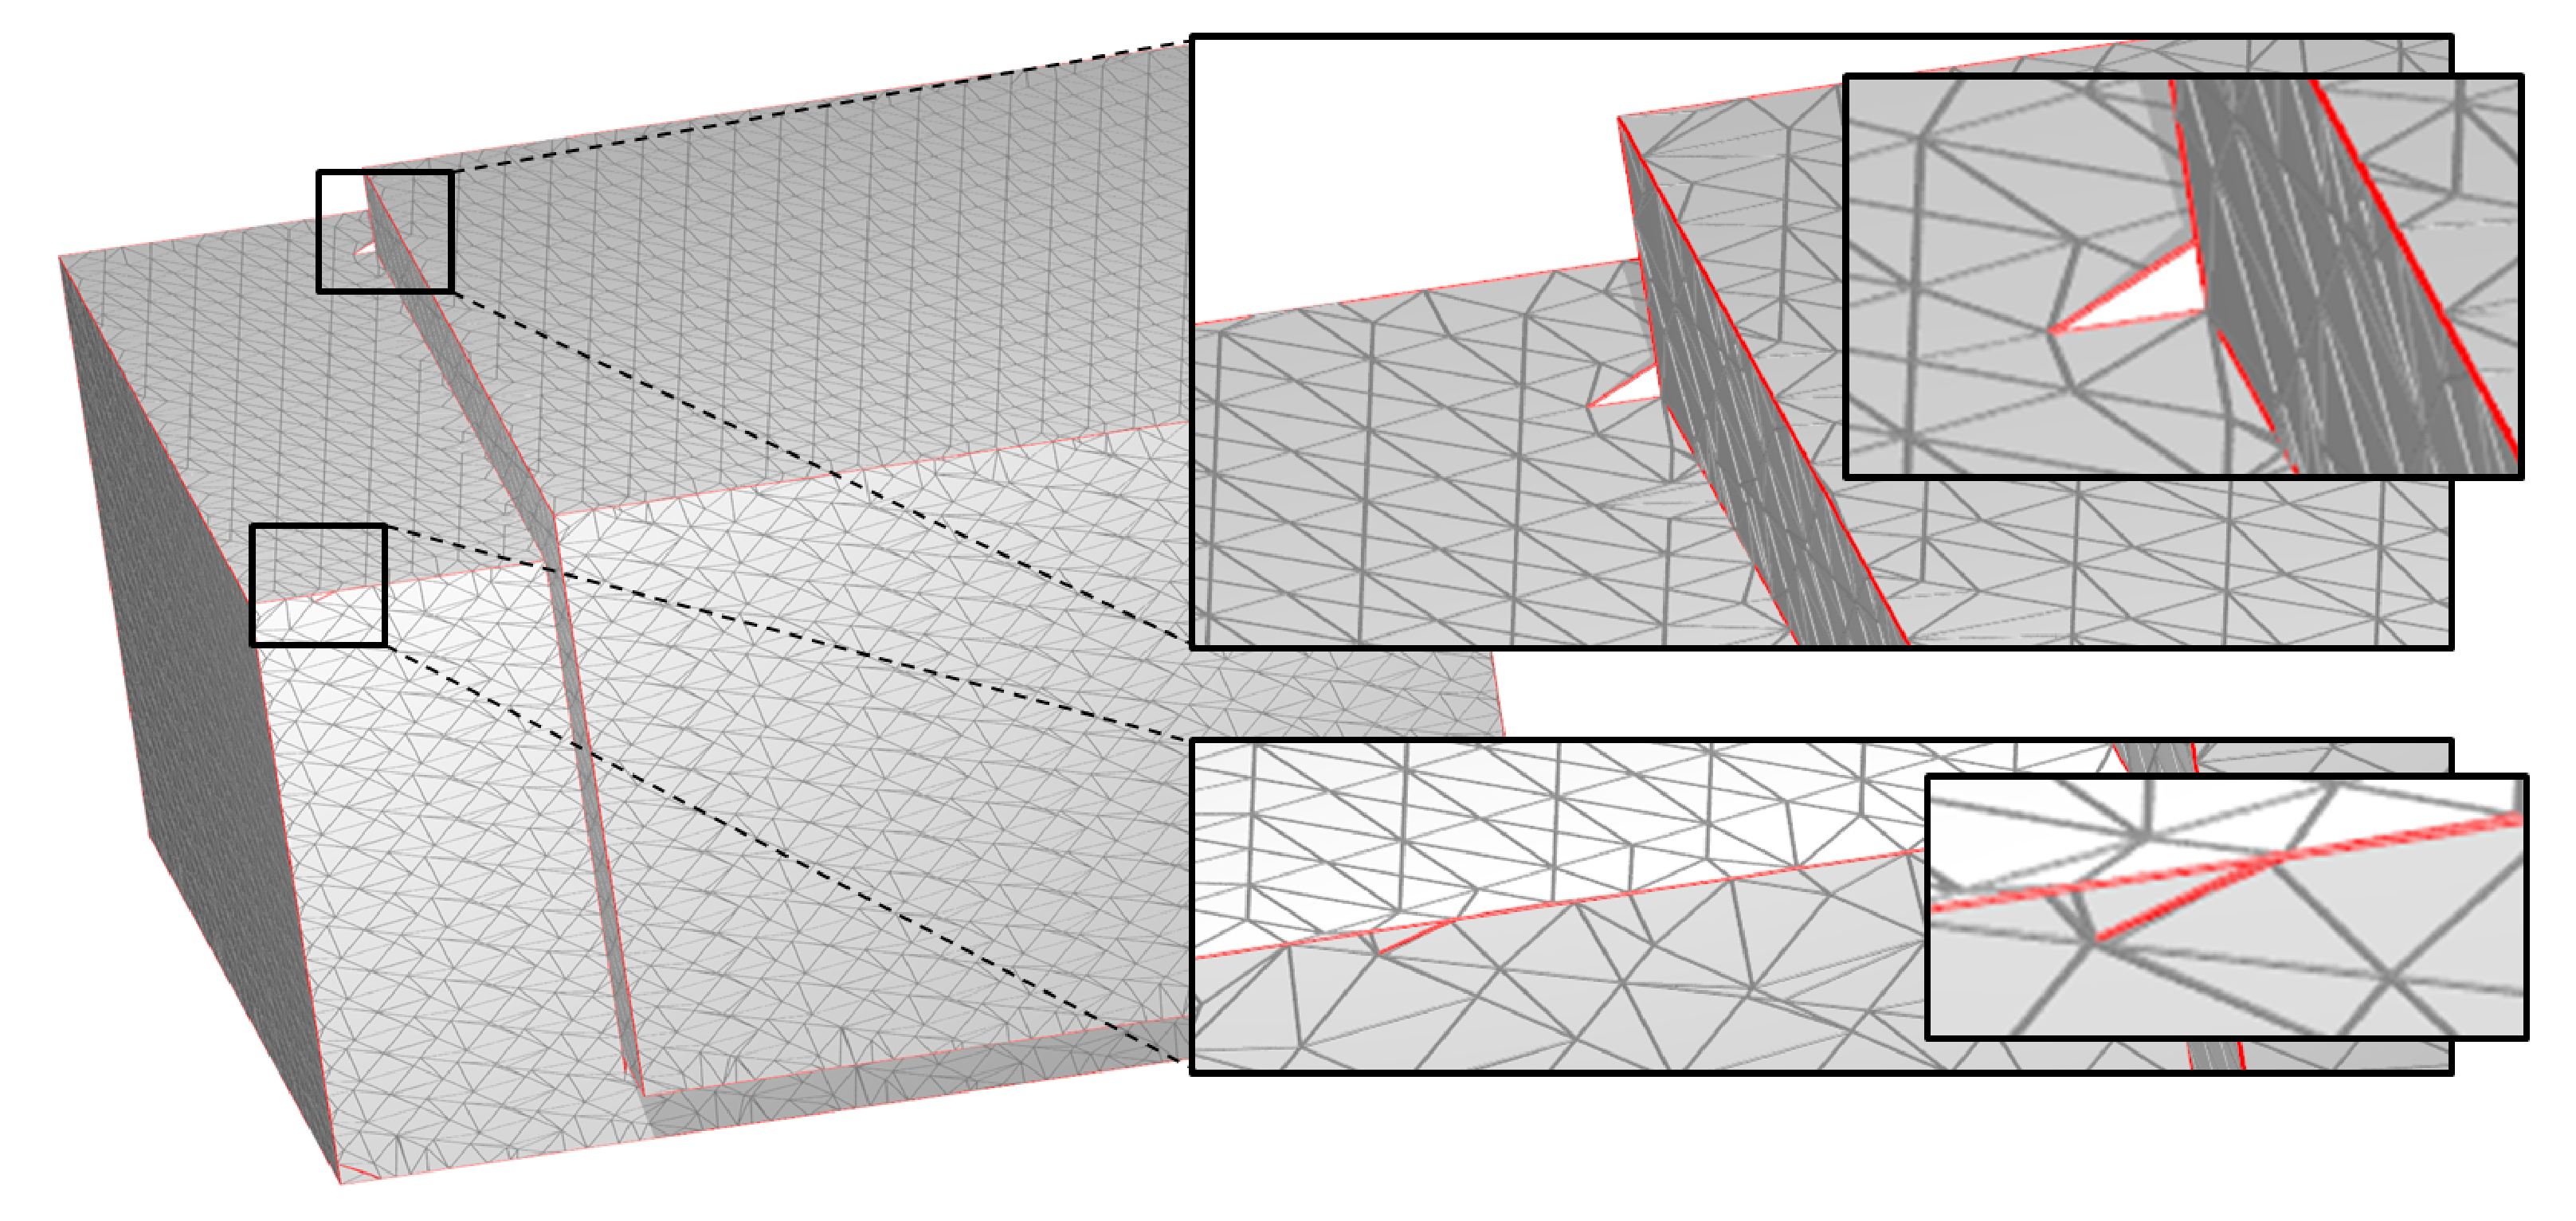
\includegraphics[width=0.5\linewidth]{images/isoExTwoCube.eps}\label{fig:isoEx:b}}\\
	%\subfloat[]{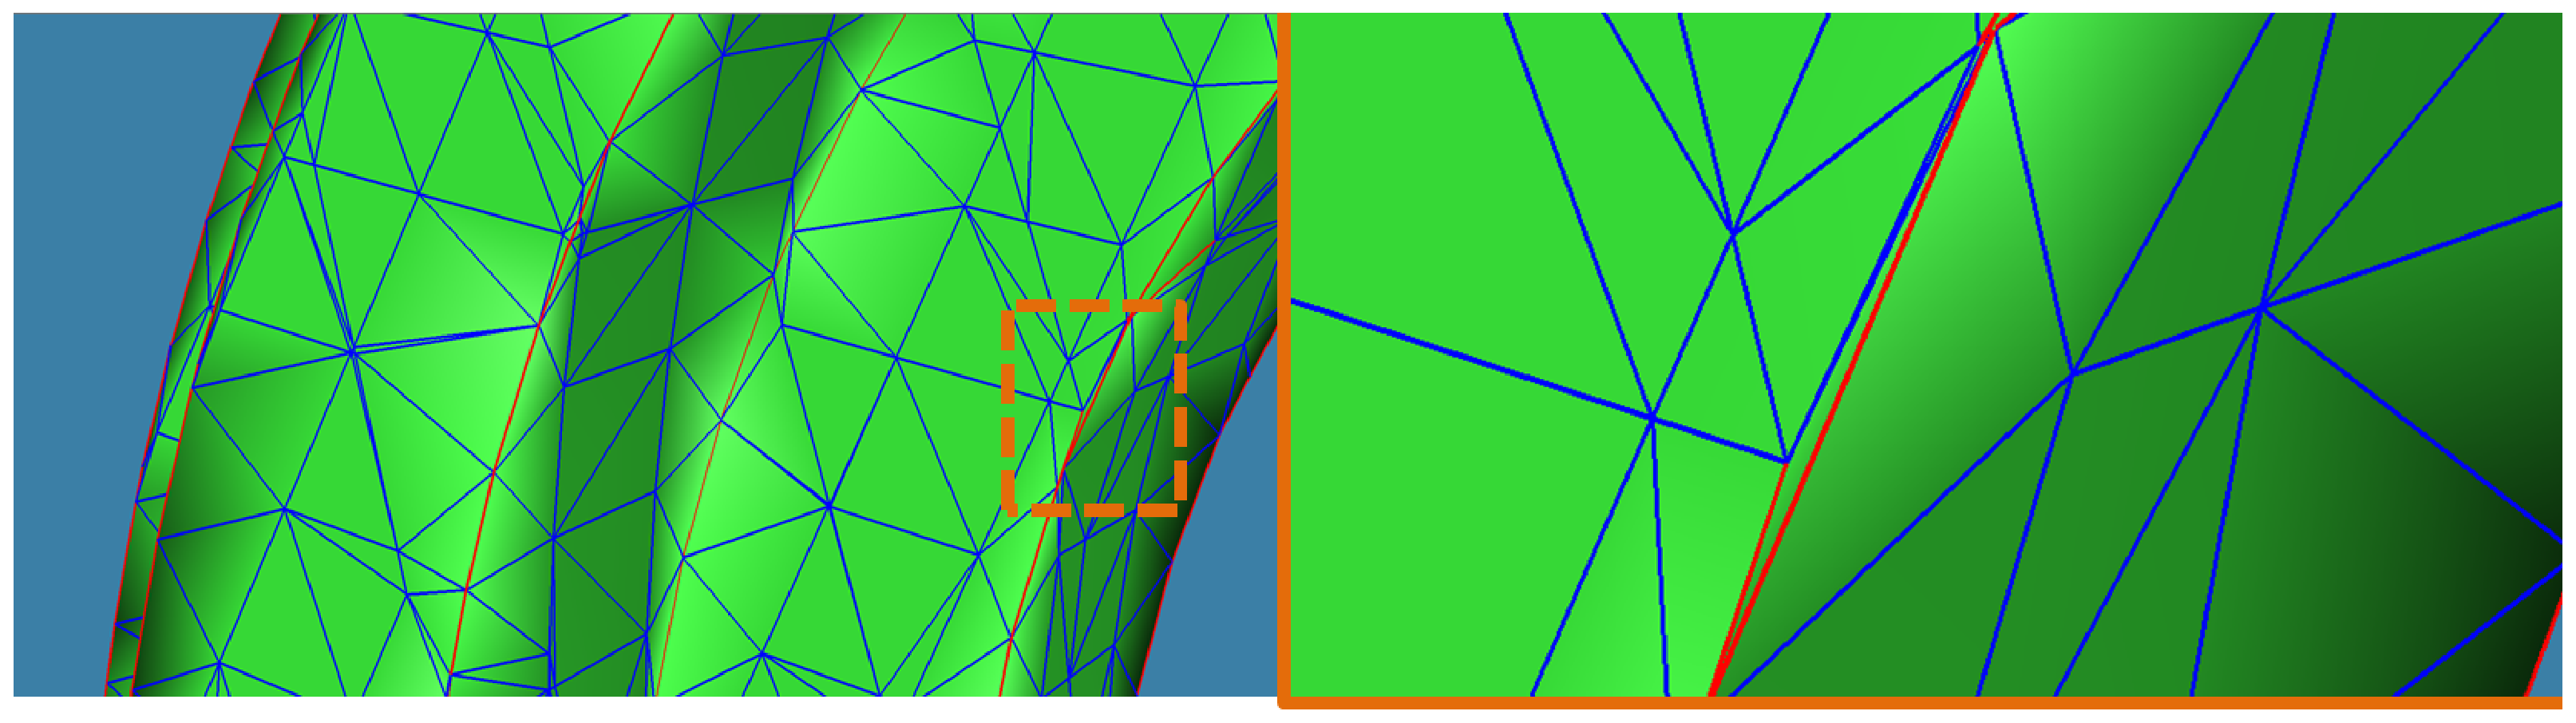
\includegraphics[width=0.45\linewidth]{images/isoex_compare1.eps}\label{fig:isoEx:a}}\quad
	%\subfloat[]{\includegraphics[width=0.45\linewidth]{images/isoEx_compare2.eps}\label{fig:isoEx:b}}
	\caption{EMCpoly (Extended Marching Cubes) and SHREC comparison.~\protect\subref{fig:isoEx_summ:a} CountDegree comparison for SHREC and extended marching cubes, 
		~\protect\subref{fig:isoEx_summ:b} Maximum angle distance for SHREC and EMCpoly,
		~\protect\subref{fig:isoEx_summ:c} angle distribution using EMCpoly, 
		~\protect\subref{fig:isoEx:a} EMCpoly on a Flange dataset, ~\protect\subref{fig:isoEx:b} on a TwoCube dataset. 
The magnified regions shows the errors generated by extended marching cubes.}	
\end{figure*}

\paragraph{Comparison with EMC (Extended Marching Cubes):}

EMC is a sample implementation of the Extended Marching Cubes algorithm by Kobbelt et al.~\cite{kbsh-fssev-01}.
The program has a function which provides the scalar value of a point cloud data set,
the directed distances along the $x$, $y$ and $z$ axes to some level set of the point cloud (a sphere),
and the gradients at query points near the level set.
Isosurfaces with sharp features are constructed by combining the functions
to represent the union, intersection or difference of balls 
defined by the point cloud data sets.

The union, intersection and difference of balls produces visually interesting surfaces
but such surfaces do not seem a realistic approximation to the surfaces found in industrial products.
To compare EMC with SHREC, we implemented functions which produce scalar values, directed distances,
and gradients, for Cube and Annulus scalar fields.
By combining these functions,
we the corresponding values for the TwoCubes and Flange scalar fields.
We added only functions to provide the relevant scalar field measurements,
but did not change the EMC code which generates the isosurface.
Our modification of EMC is called EMCpoly.

We ran EMCpoly on four Flange scalar fields with four randomly generated axes directions
and four TwoCube scalar fields with four randomly generated orientations.
We ran SHREC on eight corresponding data sets representing the same scalar fields.
Figure~\protect\subref*{fig:isoEx_summ:a} shows the countDegree
results on the test cases using both extended marching cubes and
SHREC. 
SHREC generates no countdegree errors in these testcases, in
comparison all test cases using extended marching cubes generate
degree errors; with two out of four flange datasets generating more
than 50 errors.  Example errors for flange and twoCube are shown in
Figure~\protect\subref*{fig:isoEx:a} and
Figure~\protect\subref*{fig:isoEx:b} respectively.

Figure~\protect\subref{fig:isoEx_summ:b} shows the maximum surface angle difference comparison between SHREC and extended marching cubes. The maximum surface angle difference to the synthetic mesh is less than 20$^\circ$ when using SHREC on the Flange datasets, but is around 180$^\circ$ for extended marching cubes due to triangle flipping. Finally, Figure~\protect\subref*{fig:isoEx_summ:c} shows the angle distribution for extended marching cubes on the 15 datasets, the reconstruction generates numerous simpices which are at angles greater than 50 $^\circ$ from the synthetic mesh; all the flange datasets have at least 22 triangles which have more than 50  $^\circ$ difference from the synthetic mesh, with the highest total of 45 triangles above 30 $^\circ$ for flange testcase 1.


Extensive comparison with the state of the art algorithms show that SHREC with both synthetic gradients and gradients computed from Religrad can out-perform these algorithms and reconstruct sharp features effectively. 


\begin{figure}[t] 
	%dataset t110 reconstructed from perfect mesh 
	\centering 
	\subfloat[]{\includegraphics[width=0.5\linewidth]{images/compare_cocone_perfect_mc_a.eps}\label{fig:cocone_img:a}}
		\subfloat[]{\includegraphics[width=0.5\linewidth]{images/compare_cocone_perfect_mc_b.eps}\label{fig:cocone_img:b}}
	%\includegraphics[width=\linewidth]{images/compare_cocone_perfect_mc.eps}
	\caption{Result of SingularCocone reconstruction on a TwoCube dataset. \protect\subref{fig:cocone_img:a} Input cloud is the super-sampled synthetic mesh. \protect\subref{fig:cocone_img:b} Input cloud is the super-sampled Marching Cube mesh. The magnified regions show some of the errors. The reconstruction from point cloud generated from the Marching Cube input is worse than the  point cloud from synthetic mesh input. }
	\label{fig:cocone_compare_from_perfect_1}
	\vskip-0.2cm
\end{figure} 

\begin{figure*}[t]
	\centering
		\subfloat[]{\includegraphics[width=0.3\linewidth]{images/cocone_cd_twoCube.eps}\label{fig:cocone:a}}
		\subfloat[]{\includegraphics[width=0.3\linewidth]{images/cocone_max_angle_twoCube.eps}\label{fig:cocone:b}}	
		\subfloat[]{\includegraphics[width=0.3\linewidth]{images/cocone_angle_distri_twoCube.eps}\label{fig:cocone:c}}		
		%\subfloat[]{\includegraphics[width=0.6\linewidth]{images/twoCubeQuant.eps}\label{table:cocone_compare_with_mc_table_1}}
		\caption{Cocone comparison Dey et al.~\cite{Dey2012,Dey2013}.(a) CountDegree errors on 15 datasets using SHREC with synthetic gradients, Religrad and SingularCocone. (b)Max. surface angle difference for the 15 testcases using SingularCocone and SHREC with Religrad(c) Number of triangles with angle difference of 30$^\circ$, 40$^\circ$ and 50$^\circ$ from the original mesh on a subset of 15 datasets using SingularCocone with  input points sampled from the synthetic mesh.}
		\label{fig:cocone:compare}
\end{figure*}

\paragraph{Comparison with SingularCocone.}

We compare our algorithm to the algorithm SingularCocone by Dey et al.~\cite{Dey2012}. SingularCocone reconstructs a surface with sharp edges and corners from a sampled point cloud. SingularCocone takes two inputs; one contains the point cloud, another is a weighted sampling of feature curves. Weight of the sampling will be used as weight of the protecting balls. SingularCocone generates as output a feature sensitive mesh. 

The feature curve (second input to SingularCocone) is constructed using the algorithm FeatureRecon by Dey et al.~\cite{Dey2013}. FeatureRecon extracts feature curves of a surface. The input is a point cloud sampled on the surface. FeatureRecon has two steps, feature point detection and feature curves reconstruction. 
\paragraph{Experimental details:} The input to FeatureRecon is a point cloud. We tested two different input point cloud;
\begin{enumerate}
	\item We applied Marching Cubes~\cite{lc-mchr3-87} on our datasets Sec.\ref{sec:synData}. The vertices of the mesh generated by the Marching Cubes algorithm are then super-sampled using the Monte Carlo point sampling, to generate a point cloud with approximately sixty-five thousand points.
	\item We super-sampled the synthetic meshes Sec.\ref{sec:synData}, to generate generate a point cloud with approximately sixty-five thousand points.
\end{enumerate}
The two different point clouds are used as input to FeatureRecon to extract the feature curves. 
FeatureRecon has nine separate parameters. Experimentally and also noted by the authors Dey et al.~\cite{Dey2013}, we found FeatureRecon to be heavily reliant on parameter fine tuning. We used the following parameter values for our TwoCube datasets, (as suggest by the authors Dey et al.~\cite{Dey2013}). 
$-t = 25,-fl = 0.04, -cl = 0.06, -dc = 0, -\rho3 = 0.32, -\rho1 = 0.0, -rc = 3$.

The feature curves generated using FeatureRecon along with the super-sampled point cloud is used as input to WeighCocone. For comparison test, we compare the known synthetic mesh with the output of SingularCocone.

Figure~\ref{fig:cocone_compare_from_perfect_1} shows the reconstructed mesh for one of our twoCube dataset. The associated ``sharp" edges are also shown. Figure~\ref{fig:cocone_compare_from_perfect_1}(a) shows the reconstruction from the point cloud generated from the synthetic mesh. The overlay-ed ``sharp" edges (in red) show that the reconstruction has many errors. The magnified regions show some of the errors along the sharp edges and corners. Figure~\ref{fig:cocone_compare_from_perfect_1}(b) shows the reconstruction from the point cloud generated from running Marching Cubes. The magnified regions show the same regions as Figure~\ref{fig:cocone_compare_from_perfect_1}(a). The reconstruction is worse than SingularCocone using input from synthetic mesh. 

Figure~\ref{fig:cocone:compare} shows the summary results of running weightCocone and SHREC on 15 different datasets. 
The input to weightCocone  for these tests are generated from synthetic mesh. The results from Marching Cubes input are worse and not shown.
\paragraph{}
On the same 15 datasets, we run SHREC with both synthetic gradients and using Religrad.
Figure~\protect\subref*{fig:cocone:a} shows countDegree error comparison between SingularCocone, SHREC with synthetic gradient and SHREC with gradient computed using Religrad.  SHREC with Religrad generates very few errors; only two testcases (t6 and t13 generate degree errors with a maximum of 4) , while with synthetic gradient no errors are generated. 
In contrast, SingularCocone generates a large number of errors on all the testcases; with an average of 330 errors. Figure~\protect\subref*{fig:cocone:b} shows the maximum surface angle difference from the synthetic mesh for SHREC with Religrad and WeighCocone;
The maximum angle difference is 43$^\circ$ for SHREC, with the mean error of 8$^\circ$ for the 15 tests. In comparison maximum angle difference was 87$^\circ$ for SingularCocone, with a mean of 79$^\circ$.
Figure~\protect\subref*{fig:cocone:c} shows the angle distribution for SingularCocone construction on the 15 testcases. 
On all the test cases there are large number of triangles with angle difference more than 40$^\circ$ and 50$^\circ$.

Above discussion quantitatively shows what we previously observed from  in Figure~\protect\subref*{fig:cocone_img:a},~\protect\subref*{fig:cocone_img:b} and compared to Figure~\ref{fig:flange1},~\ref{fig:shrecPerfect1} i.e sharp edges generated by SingularCocone is in general far worse than those generated by SHREC with synthetic as well as Religrad gradients. 

Dey et al.~\cite{Dey2012,Dey2013} report better results on their datasets, Which might possibly be because of parameter tuning. They themselves acknowledged as such in their work.


\begin{figure}[t]
	\centering
	\subfloat[Single image slice, original machine part]{\includegraphics[width=0.5\linewidth ]{images/cly_sleeve.1.eps}\label{fig:setA.crop1.1}}
	\subfloat[Sharp Isosurface]{\includegraphics[width=0.5\linewidth]
		{images/setA.rendering.eps}\label{fig:setA.crop1.2}}
	\caption{Motorcycle engine dataset.~\protect\subref{fig:setA.crop1.1} a slice of the original CT image, note the streaking artifacts introduced during the scanning process.
		The inset shows the original machine part. Figure \protect\subref{fig:setA.crop1.2} shows the sharp mesh.}
	\label{fig:setA.crop1}
\end{figure}


\begin{figure}[t]
\centering
	\includegraphics[width=\linewidth]{images/ictsetA_3.eps}
	\caption{SHREC with Religrad gradients computed from part of industrial CT data (Motorcycle Engine). Magnified regions show ``sharp" edges reconstructed. In red, picture from the original item.}
	\label{fig:ict:hondaEng}
\end{figure}

\begin{figure}[t]
\centering
	\includegraphics[width=\linewidth]{images/volt.eps}
	\caption{SHREC with Religrad gradients computed from part of the VOLT data. Magnified regions show ``sharp" reconstructed edges. In red picture of the original item.}
	\label{fig:ict:volt}
\end{figure}

\begin{figure}[t]
	\centering
	\subfloat[]{\includegraphics[width=\linewidth]{images/cmm.eps}\label{fig:ict:CMM:a}}\\
	\subfloat[]{\includegraphics[width=0.5\linewidth]{images/CMM.singleSliceXY.eps}\label{fig:ict:CMM:b}}
	\caption{(a) SHREC with Religrad gradients computed from part of the CMM dataset. Magnified regions show ``sharp" reconstructed edges. (b) Single slice of the CT scan, mapped to the ``heat" color map.}\label{fig:ict:CMM}
\end{figure}

\section{Experimental Results on CT Data}

We applied the SHREC algorithm on industrial X-ray computed tomography (CT)
scans of three objects.
The Motorcycle Engine data set is an industrial CT scan 
of a motorcyle engine cylinder.
The Volt data set is an industrial CT scan 
of a 440 voltage electrical connector.
The CMM data set 
is an industrial CT scan of a solid aluminum shape
used to calibrate measurements from CT scans.
CMM stands for ``coordinate measuring machine''.
Data set sizes, isovalues and average surface sizes are presented
in Table~\ref{table:datasets}.
Since the CT scanner provides only scalar values for each object,
we used Religrad to construct gradients at the grid vertices.

The full Motocycle Engine data set has very large ??? dimensions.
Figure~\ref{fig:ict:hondaEng} shows a small corner of the original object
(red box)
and the results of reconstruction of that corner.
The magnified regions (with black border) show that the sharp edges
are well reconstructed. In yellow border boxes, we see magnified parts
of the reconstructed mesh along with the sharp and non-sharp edges
generated by SHREC.
The isosurface statistics and timing reported in Table~\ref{table:datasets}
are only for the small $411 \times 431 \times 61$ subregion of the data
depicted in Figure~\ref{fig:ict:hondaEng}.

Figure~\ref{fig:ict:volt} shows part of the 440 voltage connector (in red)
and the SHREC reconstruction of the Volt dataset.
To aid in visualization of the sharp features,
the figure displays a cropped image of the the reconstructed isosurface.
Once again we see that SHREC is able to reconstruct 
the sharp (flange-like) curves accurately.

Figure~\ref{fig:ict:CMM} shows the SHREC reconstruction of the CMM data set.
Again, the reconstructed isosurface is cropped to better
display the sharp features.
Figure~\protect\subref*{fig:ict:CMM:b} shows a single slice of
the CT scan, mapped to the ``heat" color map.

Through these reconstructions and others,
we have confirmed that SHREC performs well on industrial CT data sets. 

\section{Timings}

